  
\RequirePackage[l2tabu, orthodox]{nag}

\documentclass[publish, glossary]{thesis}

\def\UrlBreaks{\do\/\do-}

\usepackage{array}
\newcolumntype{P}[1]{>{\centering\arraybackslash}p{#1}}

\usepackage{amsmath, amsfonts, amsthm, amssymb, commath}
\usepackage{boxedminipage, xspace}   
\usepackage[T1]{fontenc}
\usepackage{changepage}
\usepackage[export]{adjustbox}

\usepackage{graphics, graphicx}
\usepackage{subfig}

\usepackage{booktabs}
\usepackage{multirow}
\usepackage{parcolumns}
\usepackage[roman]{parnotes}
% \usepackage{paralist}
\usepackage{tabu}
\usepackage{makecell}
\usepackage{booktabs,multicol,multirow,graphicx,tabularx,ragged2e,dcolumn}
\usepackage{tablefootnote}

% \usepackage{algorithm}
\usepackage{algorithmic}
\usepackage[ruled,vlined]{algorithm2e}

\usepackage{color}
\usepackage{tcolorbox}
\usepackage{listings}
\usepackage{framed}
\usepackage{upquote}

\usepackage{setspace}
\usepackage{enumitem}
\usepackage{nicefrac}


\newcommand{\etal}{\emph{et al}.\@\xspace}
\newcommand*{\aka}{\emph{a.k.a.}\@\xspace}
\newcommand{\jj}[1]{\textcolor{blue}{JJ: #1}}
\newcommand{\formulas}{formul\ae\xspace}
\newcommand{\linebreakand}{%
  \end{@IEEEauthorhalign}
  \hfill\mbox{}\par
  \mbox{}\hfill\begin{@IEEEauthorhalign}
}

\definecolor{keyword}{RGB}{127,0,0}
\definecolor{block}{RGB}{0,127,0}
\definecolor{variable}{RGB}{0,0,127}
\definecolor{editorGray}{rgb}{0.95, 0.95, 0.95}
\definecolor{editorOcher}{rgb}{1, 0.5, 0} 
\definecolor{editorGreen}{rgb}{0, 0.5, 0}
%FlakyCat
\definecolor{codegreen}{rgb}{0,0.6,0}
\definecolor{codegray}{rgb}{0.5,0.5,0.5}
\definecolor{codepurple}{rgb}{0.58,0,0.82}
\definecolor{backcolour}{rgb}{0.95,0.95,0.95}
\definecolor{Gray}{gray}{0.9}

\lstdefinestyle{mystyle}{
    backgroundcolor=\color{backcolour},   
    commentstyle=\color{codegreen},
    keywordstyle=\color{magenta},
    numberstyle=\tiny\color{codegray},
    stringstyle=\color{codepurple},
    basicstyle=\ttfamily\footnotesize,
    breakatwhitespace=false,         
    breaklines=true,                 
    captionpos=b,                    
    keepspaces=true,                 
    numbers=left,                    
    numbersep=5pt,                  
    showspaces=false,                
    showstringspaces=false,
    showtabs=false,                  
    tabsize=2
}

\lstset{
numbers=left,
stepnumber=1,
numbersep=5pt,
xleftmargin=0pt,
xrightmargin=0pt,
breaklines=true,
escapeinside={<@}{@>},
numberstyle=\color{black},
columns=fixed,
keepspaces=true,
columns=flexible,
framesep=0pt,
frame=single,
basicstyle=\ttfamily\footnotesize
}


\newglossaryentry{api}
{
	type=\acronymtype,
	name={API},
	description={Application Programming Interface},
	first={Application Programming Interface (API)}
}

\newglossaryentry{bnf}
{
	type=\acronymtype,
	name={BNF},
	description={Backus–Naur Form},
	first={Backus–Naur Form (BNF)}
}

\newglossaryentry{css}
{
	type=\acronymtype,
	name={CSS},
	description={Cascading Style Sheet},
	first={Cascading Style Sheet (CSS)}
}

\newglossaryentry{dag}
{
	type=\acronymtype,
	name={DAG},
	description={Directed Acyclic Graph},
	first={Directed Acyclic Graph (DAG)}
}

\newglossaryentry{dom}
{
	type=\acronymtype,
	name={DOM},
	description={Document Object Model},
	first={Document Object Model (DOM)}
}

\newglossaryentry{gdpr}
{
	type=\acronymtype,
	name={GDPR},
	description={General Data Protection Regulation},
	first={General Data Protection Regulation (GDPR)}
}

\newglossaryentry{gui}
{
	type=\acronymtype,
	name={GUI},
	description={Graphical User Interface},
	first={Graphical User Interface (GUI)}
}



\newglossaryentry{html}
{
	type=\acronymtype,
	name={HTML},
	description={Hypertext Markup Language},
	first={Hypertext Markup Language (HTML)}
}

\newglossaryentry{kdt}
{
	type=\acronymtype,
	name={KDT},
	description={Keyword-Driven Testing},
	first={Keyword-Driven Testing (KDT)}
}

\newglossaryentry{kpi}
{
	type=\acronymtype,
	name={KPI},
	description={Key Performance Indicator},
	first={Key Performance Indicator (KPI)}
}

\newglossaryentry{mbt}
{
	type=\acronymtype,
	name={MBT},
	description={Model-Based Testing},
	first={Model-Based Testing (MBT)}
}

\newglossaryentry{qa}
{
	type=\acronymtype,
	name={QA},
	description={Quality Assurance},
	first={Quality Assurance (QA)}
}

\newglossaryentry{rdbms}
{
	type=\acronymtype,
	name={RDBMS},
	description={Relational Database Management System},
	first={Relational Database Management System (RDBMS)}
}


\newglossaryentry{sut}
{
	type=\acronymtype,
	name={SUT},
	description={System Under Test},
	first={System Under Test (SUT)}
}

\newglossaryentry{suit}
{
	type=\acronymtype,
	name={SUIT},
	description={System User Interactive Test},
	first={System User Interactive Test (SUIT)}
}

\newglossaryentry{url}
{
	type=\acronymtype,
	name={URL},
	description={Uniform Resource Locator},
	first={Uniform Resource Locator (URL)}
}

\newglossaryentry{vgt}
{
	type=\acronymtype,
	name={VGT},
	description={Visual GUI Testing},
	first={Visual GUI Testing (VGT)}
}



\newglossaryentry{w3c}
{
	type=\acronymtype,
	name={W3C},
	description={World Wide Web Consortium},
	first={World Wide Web Consortium (W3C)}
}

\newglossaryentry{whatwg}
{
	type=\acronymtype,
	name={WHATWG},
	description={Web Hypertext Application Technology Working Group},
	first={Web Hypertext Application Technology Working Group (WHATWG)}
}



\newglossaryentry{xml}
{
	type=\acronymtype,
	name={XML},
	description={eXtensible Markup Language},
	first={eXtensible Markup Language (XML)}
}
\typeout{}
\addbibresource{references.bib}

\begin{document}		
	\frontmatter
	\pagenumbering{gobble}
	
	\thispagestyle{empty}
\newgeometry{left=2cm,right=2cm,top=2cm,bottom=0.1cm}

\begin{center}         
         
\includegraphics[width=0.2\linewidth]{figures/logo/logoul.pdf}
         \vspace{0.3cm}\noindent
%         \texttt{PhD-FSTC-2016-43}
         
         The Faculty of Science, Technology and Communication
         
         \vspace{1cm}\noindent
         {\LARGE \textbf{\textsc{Dissertation}}}
         
         \vspace{0.5cm}
         \noindent
         Defense held on September $15^{th}$, 2021 in Luxembourg
         
         \vspace{0.5cm}\noindent
         to obtain the degree of
         
         \vspace{0.8cm}\noindent
         {\large \textbf{\textsc{Docteur de l'Université du Luxembourg en Informatique}}}

         \vspace{0.5cm}\noindent
         {\Large by}

         \vspace{0.5cm}\noindent
         {\Large Renaud \textsc{Rwemalika}}\\
%         {\footnotesize Born on $24^{th}$ November 1992 in Libourne (France)}

         \vspace{1cm}\noindent
         {\LARGE \textbf{\textsc{On the Maintenance of}}}\\[0.4cm] 
         {\LARGE \textbf{\textsc{System User Interactive Tests}}}\\[0.4cm]
\end{center}

\vspace{0.4cm}

\begin{adjustwidth*}{1em}{1em}

\noindent
\textbf{\large Dissertation defence committee}
%\normalsize\textit{(Waiting for approval)}


\vspace{0.2cm}
\noindent
Dr.  Marinos \textsc{Kintis}, advisor\\
{\small \emph{Senior Data Engineer, FanDuel, United Kingdom}}   

\vspace{0.2cm}
\noindent
Dr. Michail \textsc{Papadakis}, advisor\\
{\small \emph{Lecturer, University of Luxembourg, Luxembourg, Luxembourg}}   

\vspace{0.2cm}
\noindent
Prof. Dr. Yves \textsc{Le Traon}, supervisor\\
{\small \emph{Professor, University of Luxembourg, Luxembourg, Luxembourg}}

\vspace{0.2cm}
\noindent
Prof. Dr. Myra \textsc{Cohen}, supervisor\\
{\small \emph{Professor, Iowa State University, Ames, Iowa}}

\vspace{0.2cm}
\noindent
Prof. Dr. Anna Rita \textsc{Fasolino}, supervisor\\
{\small \emph{Professor, Iowa State University, Luxembourg, Luxembourg}}

\end{adjustwidth*}

\restoregeometry
	
	\linenumbers
	\chapter*{Abstract}

Many companies rely on software testing to verify that their software products meet their requirements. However, test quality and, in particular, the quality of tests interacting with the \gls{gui}, i.e. \gls{suit}, is hard to achieve. The problem becomes challenging when the \gls{sut} evolves, as \gls{suit} suites need to adapt and conform to the evolved software. Indeed, because the user interface is a part of the system that tends to undergo rapid evolutions, \gls{suit}s are particularly prompt to break.

In this dissertation, we present an empirical evaluation of the impact of the evolution and the maintenance of SUIT suites. We aim to demonstrate the problem of test maintenance and overall improve the understanding of SUIT scripts evolution. To that end, we identify, collect and analyze test code changes across the evolution of an industrial test suite. We show that the problem of test maintenance is largely due to test fragility (most commonly performed changes are due to locator and synchronization issues) and bad practices (over 30\% of keywords are duplicated). 

To further investigate the question of bad test code practices such as test clones, we perform a multivocal study to identify which bad practices, i.e. SUIT smells, are already studied in both industry and academia establish a list of 35 test code smells. For 16 of them, we derive metrics to analyze their diffusion across tests as well as potential refactoring actions removing the test code smells. Conducting a second empirical study, including both industrial and open-source test suites, we show that test code smells are largely present in \gls{suit}s, potentially contributing to the fragility and hindering the maintenance process. Interestingly, when observing refactoring actions, they remain rare during the lifespan of the tests. Yet, symptoms tend to disappear as old tests are discarded and new ones are introduced.

However, during the analysis of SUIT smells, we observe that bad practices impacting locators do not appear often in the test code. This observation contrasts with the analysis of the evolution of the SUIT presented in our first empirical study.  This apparent contradiction arises from the limitation of property-based locators which rely on the structure of the representation layer of the \gls{sut}. Thus, such approaches are sensitive to internal iso-functional changes occurring during the normal evolution of the \gls{sut}. To account for this limitation, we introduce a new way of expressing locators, HPath. Instead of relying on the internal representation of the GUI, HPath relies on its rendered characteristics. Our results suggest that despite what is presented in the literature on smells, locators relying on a smaller number of GUI elements to fully qualify a target do not necessarily lead to more robust locators. On the contrary, the choice of the GUI element properties seems to play a stronger role in the robustness to change.

Overall, this dissertation provides insights into how \gls{suit}s evolve and shows that \gls{suit} fragility plays a major role in the associated maintenance effort. It also proposes techniques that effectively facilitate the maintenance with the early detection of sub-optimal patterns and the introduction of a locator representation more robust to \gls{sut} evolution.
	
	\chapter*{Acknowledgments}

Embarking on the arduous yet exhilarating journey of a PhD, one finds himself traversing an emotional rollercoaster of intellectual growth, self-discovery, and relentless perseverance. Approaching its conclusion, I realise now how well-surrounded I was throughout these four years I spent in the SerVal team of the SnT research centre. Here, I want to say a few words to those who took an important part in this adventure and had positive impacts on it.

Yves, these first words go for you. As my official supervisor, you trusted me since the very first time we met and you gave me all the keys I needed to successfully pursue my PhD. I am thankful for your support and your constant positive thinking.

Mike, you were my direct supervisor and when I joined the team I didn't fully measure its excellence. You are largely contributing to it and I learned so much from you. I am grateful for all your counselling, help and every one of the discussions we had. I admire the amount of work you give to create this wonderful research environment.

Sarra, our paths met at a crucial point in my life. I was not expecting your arrival in our team nor that I would benefit from the additional support and expertise of a young researcher. I am deeply thankful for your guidance and cooperation. You genuinely inspired me and will continue to do so for a long time.

Maxime, while you were expanding the domains of expertise in our team, you always remained available and supportive to me. I sincerely appreciate your dedication and I will keep good memories of the discussions we had.

I would like to thank all my co-authors for their involvement and feedback in the different projects. Thanks also to the jury members for the time and interest they gave to my research. This dissertation would not have been the same without your help. I also want to express my gratitude towards all my fellow SerVal colleagues, some arrived, and some left through my journey but all contributed to creating a fantastic place to conduct research. I hope we will stay in touch.

On a more personal note, I wish to thank my family for their support: my mom, who listened so many times to my work-related stories, my dad, who doesn't know how important he is to me and my brother, whose presence has the magical ability to always transport me back to the carefree days of childhood. You are the joy of my life. Finally, I thank all my friends with whom I was able to temper the most stressful part of this adventure.
	\tableofcontents
	
	\cleardoublepage
	
	\mainmatter	
	
	\chapter{Introduction}
\label{chap:introduction}

\chapterPage{
With GUI-based applications becoming ubiquitous as a mean for users to interact with software, the question of their correctness is of utmost importance. Yet, testing such applications still poses major challenges to practitioners. 
After introducing four approaches employed when creating \gls{suit}, we introduce the challenges that come with them.
Before describing the three contributions of this dissertation, we scope the addressed sub-challenges tackled.
}

Today, companies need to produce software faster than ever in order to remain competitive. To do so, they rely mainly on two different strategies: the integration of a continuous deployment pipeline and the establishment of agile methodologies within the company. These strategies allow software producers to increase the release rate while maintaining a high quality for the software that is shipped.

One of the keystones of the quality process is based on the adoption of strategies to assess that both functional and technical requirements are met. Because of the complex dynamic runtime of most modern applications, static analysis techniques face limitations in revealing violations of the requirements. Thus, most teams heavily rely on testing to reveal faults in their software. 

We define testing as a technical investigation to assess the quality of a \gls{sut} by executing the latter against a set of input values. Tests can further be classified through the scope they target into three main categories: unit, integration, and system tests. Unit testing covers the tests that are testing a unit in isolation, be it a class, a function, or any other software component,  to validate each unit individually. In integration testing, related units are grouped together and tested as a group. Finally, system testing covers the tests evaluating the system as a whole to ensure its compliance with its requirements.

Because unit and integration tests target more restricted portions of the application, they offer better control to the tester who can isolate functionalities from its environment and tests specific behaviors of the system sub-parts. On the other hand, system tests, and especially those interacting with the user interface, target the system as a whole (usually as a black box). Therefore, they are sensitive to any change in the \gls{sut} and its interface. This property makes system tests more fragile, \ie\ they may break as a result of non-functional changes that are not targeted by the test.

In this work, we analyze the evolution of those system tests interacting with the user interface to shed light on the reasons why these tests require costly maintenance \cite{Alegroth2016, Coppola2020}. Then, we propose some solutions as to how to create more robust test suites, \ie test suites that are less likely to break following non-functional evolutions of the \gls{sut}.

\section{GUI Testing}
\label{sec:introduction-gui-testing}

User Interfaces are designed to provide a mean for the user to interact with an application. Unfortunately, as interfaces become more user-friendly, the underlying technology becomes more complex \cite{Myers1994}. Indeed, as depicted by \textcite{Myers1995}, user interfaces require the system to  interact with complex graphical components, to provide multiple ways to provide the same command, to manage multiple asynchronous input devices through the use of asynchronous event loops, or to provide an interactive computer programming environment (\eg\ read–evaluate–print loop). To ease development, the literature introduces different architectural designs to decouple the code responsible for the user interaction from the rest of the system such as the Entity-Component-System model \cite{Raffaillac2018} or the Model-View-Controller \cite{Krasner1988}.

Nevertheless, while these architectural solutions offer advantages by providing better isolation when testing individual components, in the case of system testing, the challenges remain open. Indeed, as the complexity of user interfaces and their associated code continues to grow, testing through the user interface for functional correctness remains challenging, but vital to help ensure the safety, robustness, and usability of the \gls{sut}.

Furthermore, today, \gls{gui} are becoming ubiquitous as a mean for users to interact with a software application \cite{Myers1992, Myers1995, Brooks2009, Memon2010}. In this work, we define a \gls{gui} as a hierarchical, graphical front-end to a software system that accepts as input user-generated and system-generated events from a fixed set of events that result in graphical output \cite{Memon2007} and/or alter the state of the software \cite{Nguyen2014}. A \gls{gui}-based application is a software for which the \gls{gui} is the main mode of interaction to the detriment of other types of user interfaces. As a consequence of the predominance of \gls{gui}-based applications, a lot of effort has been geared towards \gls{gui} automation, notably focusing on desktop applications \cite{Nguyen2014, Advolodkin2018, Pezze2018}, web applications \cite{Mesbah2009, Biagiola2019}, mobile applications \cite{Machiry2013, Gomez2013, Mao2016, Salihu2019, Yu2019} or cross-platform applications \cite{Canny2020}. However, as we show later in this section, major challenges remain open.

The question of the correctness of a \gls{gui}-based application is of utmost importance since prototyping and developing the behavior of a system is harder than prototyping and developing the appearance of the application \cite{Myers2008}. It is in this context that we introduce \gls{gui} testing which encompasses the techniques used to test user interface layout and its behavior. More precisely, \gls{gui} testing can be defined as ``the process of testing a software application with a graphical front-end to guarantee that it meets its specification by performing a sequence of events against the \gls{gui} elements'' \cite{Cunha2010, Banerjee2013, Issa2012}. Thus, relying only on stimuli inputs and output reactions, a \gls{gui} test is considered as a black-box test. Additionally, we define a \gls{suit} as an automated \gls{gui} test that exercises the \gls{sut} as a whole (system level). Note that in this work focusing on automated system-level test interacting with the \gls{sut} through its \gls{gui}, we use \gls{gui} test and \gls{suit} interchangeably.

Strategies have been developed to exercise the user interface to ensure that functional requirements are satisfied. Different techniques have been proposed but all rely on the same principle. A test framework executes events belonging to \gls{gui} components and monitors the resulting changes to the program state \cite{Nguyen2014}. In other words, each technique generates a sequence of test step, that will be executed against the \gls{sut} (input) and captures some indication as to what is the current state of the system (output). Each test step consists of a triple: (1) an action to be performed, (2) the \gls{gui} element on which to perform the action, and (3) an optional value passed to the element. Consequently, a natural classification discriminates each strategy on the way the sequence of test steps is generated.

In the remainder of this section, we discuss current techniques used to generate \gls{suit}s. The techniques are ordered based on their theoretical potential for automation during the test generation process.

\subsection{Random GUI Testing}
\label{sec:introduction-random-gui-testing}

In random \gls{gui} testing, also known as monkey testing or random-walk, tests are automatically created by generating sequences of events at random in the hope of exploring the \gls{sut} to reveal failures. Because no requirements are passed as input such techniques rely on specific constraints that are application or domain invariant oracles \cite{Mesbah2009} to assess correctness. Thus, any sequence of events that causes the \gls{sut} to violate an invariant is considered as a fault revealing test case \cite{Barr2015}. These properties make random \gls{gui} testing cheap to run on a large number of versions/configurations of applications.

Typically, such tools rely on the concept of fuzz testing which performs arbitrary or contextual events against the SUT. Tools like Monkey \cite{Google2020},  ATUSA \cite{Mesbah2012} or Dynodroid \cite{Machiry2013} rely on pseudo-random input events which include both user interface events and system events and assess the generated sequences against invariant oracles. 

One of the major challenges encountered when relying on random \gls{gui} testing resides in the exploration of the application states. Indeed, with modern applications, the infinite number of combinations of user inputs leads to a potentially large and sometimes infinite number of reachable states. Consequently, the search space cannot be covered exhaustively leading to potentially low state coverage \cite{Canny2019}. Furthermore, in the case of more complex input, such as a chain of character, randomly generated input have often low chances of producing feasible test cases, thus requiring a large number of input generations to find interesting test cases (\eg if a login page exists, only a combination of a valid user name and password would allow the test case to continue its exploration behind the login wall).

To alleviate these limitations, different approaches emerged introducing algorithms relying on heuristics to better explore the application state space and consequently generate more fault-revealing test cases. For example, EXSYST \cite{Gross2012}, EvoDroid \cite{Mahmood2014} and Sapienz \cite{Mao2016} propose to use search-based algorithms to explore the space of possible sequences and generate tests for Android applications while Dynodroid \cite{Machiry2013} exploits machine learning algorithms to achieve the same goal. The goal of the algorithm is to generate short sequences of input while improving coverage (code \cite{Gross2012} and/or state \cite{Machiry2013} coverage) to produce fault-revealing sequences. More recently, tools such as DIG \cite{Biagiola2019} try to increase the coverage by specifically targeting the input generation problem. While these approaches look promising, today, monkey testing requires the user to provide some inputs (\eg login and passwords) to allow the algorithms to explore more states.

To summarize, random \gls{gui} testing offers a cheap alternative to classical test scripting which can be useful to detect crashes and other invariants in an exploratory fashion. Nevertheless, because of the lack of knowledge of the functional requirements and the lifecycle of the application, exploring the application and covering hidden behaviors remains challenging. Thus, while companies do use random \gls{gui} testing, they use it in addition to other techniques that we present below.

\subsection{Model-Based Testing}
\label{sec:introduction-model-based-testing}

\gls{mbt} is an approach encompassing the processes and techniques for the automatic derivation of abstract test cases from abstract models \cite{Utting2012}. Functional specifications of a system, with the assumption that they are precise enough, are used as input to design process models which in turn are used to generate automated test cases \cite{Gupta2011}. This process can be devised in the five below steps \cite{Utting2012}:

\begin{enumerate}
    \item A model of the \gls{sut} is built from informal requirements or existing specification documents;
    \item Selection criteria are chosen, to guide the automatic test generation;
    \item Test selection criteria are transformed into test case specifications;
    \item A set of test cases is generated with the aim of satisfying all the test case specifications;
    \item Finally, the test cases are executed against the \gls{sut}.
\end{enumerate}

Unfortunately, most of the current \gls{gui}-based applications are not derived from a model, thus, cannot rely on an \emph{a priori} model encompassing all the expected behaviors of the application. Besides, even though advances have been made in Model-Based Software Engineering, complex \gls{gui} applications exhibit behaviors that cannot be expressed by models found in \gls{gui} testing \cite{Lelli2015}. This limitation causes \gls{mbt} to offer limited applicability which explains why practitioners shy away from the model-based solutions proposed in the scientific literature.

To tackle this shortcoming, researchers propose methods to automatically derive a model of the application by reverse engineering, thus, using techniques similar to the ones presented in Section~\ref{sec:introduction-random-gui-testing}. For example, \textcite{Memon2007} introduces an event-flow model to formally represent events and event interactions in a \gls{gui}-based application. However, because of the large space of events and interactions present in a given application, manually building the model is prohibitive. Thus, the author proposes to rely on reverse-engineering to automatically derive the models by automatically exploring applications (in a similar fashion as random \gls{gui} testing). Unfortunately, models built that way do not guarantee completeness, leading to difficulties such as assessing if the coverage offered by the model is sufficient or choosing inputs during exploration. While recent literature offers partial solutions such as improving the input generation \cite{Biagiola2019} or new ways to derive models from the \gls{gui} and its requirements \cite{Canny2020} the question of automatic exploration of modern \gls{gui}-based application remains an open problem.

\subsection{Record \& Replay}
\label{sec:introduction-record-and-replay}

This leads us to the third category of \gls{gui} testing, Record \& Replay which generates test cases from sequences of user interactions provided by the tester and not by exploring the model in a random fashion (Random \gls{gui} Testing) or by relying on a model (Model-Based Testing). As its name suggests, Record \& Replay works in two phases: a record phase and a replay phase:

\begin{enumerate}
    \item During the record phase, the tester manually interacts with the application, thereby generating events on the \gls{sut}. The tool records the interactions and a part of the \gls{sut} response state as specified by the tester.
    \item During the replay phase, the recorded test cases can be replayed on subsequent versions of the \gls{sut} and the captured state of the application are used as test oracles.
\end{enumerate}

The generated test cases require human intervention during the capture phase and can be rerun, reducing the overall effort of regression testing. Furthermore, because the test cases are generated by the framework, no particular skills are needed from the tester. \textcite{DiMartino2021} show that even when human testers have limited information about the system, they achieve better coverage metrics than automatic test generation techniques when using Record \& Replay.

Despite its advantages when generating the test cases, the generated tests tend to be fragile \cite{Hammoudi2016}. Indeed, whenever the application naturally evolves, the generated test cases might break, requiring testers to regenerate the test. This limitation can be exacerbated by agile and continuous delivery practices where applications and their user interfaces are under constant evolution.

To address this drawback, the research community proposes different ways to tackle the problem of fragility. Some attempts have been geared towards generating more robust test cases \cite{Hammoudi2016b}. Other researchers focus their attention on the more efficient way to record the interaction \cite{Ronsse1999}. Finally, instead of recording the interactions as sequences of actions, tools such as EventFlowSlicer \cite{Saddler2017} generate a model from these interactions. Thus, similarly to \gls{mbt}, subsequent versions are tested against the model.

Therefore, we see that while the generation of test cases using Capture \& Replay is efficient, the approach suffers from drawbacks in terms of the maintainability of the generated test suite. This issue is all the more relevant as the generated tests are often obscure, lacking any type of internal hierarchy, thus, compromising any attempt to manually fix such tests. 

\subsection{Test Scripting}
\label{sec:introduction-test-scripting}

Finally, the last technique covered in the section covers tests that are manually crafted by testers themselves. Following the general definition, a test script can be defined as a piece of executable code that executes a test case against the \gls{sut} and generates a verdict. In this work, we focus on test scripts interacting with the \gls{sut} through their \gls{gui}, namely, \gls{suit} scripts. \gls{suit} scripts aim at separating test design from the technical implementation of the tests.

Indeed, \gls{suit} scripts are typically used by teams performing acceptance testing. Acceptance tests ensure that a specific acceptance criterion, which can be functional or non-functional is met \cite{Pandit2015}. Conforming to the acceptance criteria both verifies that the \gls{sut} delivers the business value expected by the customer and guards against regressions or defects that break preexisting functions of the \gls{sut} \cite{Humble2010}. Hence, acceptance tests are not concerned with the internal implementation of the \gls{sut}, but with its overall behavior. Additionally, because such tests are business-facing, they are involved in the discussion between testers, developers, and business analysts, and, as such, should be readable by all stakeholders.

Practitioners propose design patterns to separate different concerns into different abstraction layers. For example, \textcite{Humble2010} propose the three following layers adopted by open-source and commercial tools like Robot Framework, Cucumber, JBehave, Finess, or TestComplete:

\begin{itemize}
    \item \textbf{Acceptance Criteria.} It contains functional behavior, quality characteristics, scenarios, or business rules that the test is targeting. These are usually written in a form close to natural language. The goal of this layer is to express for all the stakeholders the requirements that are being automatically executed.
    
    \item \textbf{Test Implementation Layer.} It contains all the underlying implementation of the test called by the acceptance criteria layer. Because test implementations that refer directly to the application \gls{gui} elements are fragile, it is not uncommon to see large portions of acceptance test suites break when a single \gls{gui} element changes. While deferring the interactions with the application to the application driver layer does not make tests more robust to changes, it will make their maintenance easier with a better separation of concerns. Indeed, this layer follows the logic and vocabulary of the \gls{sut}, instead of the technical details of the implementation with its \gls{gui} elements.
    
    \item \textbf{Application Driver Layer.} It is the layer that understands how to interact with the \gls{sut}. While the two other layers use only the domain language of the business, the application driver layer is expressed in the domain language used by the drivers that communicate with the \gls{sut}. One of the consequences of a well-designed application driver layer is to improve test reliability. Moreover, because of the high degree of reuse that is implicit when relying on an application driver layer, complex interactions and operations can be written once and used in many tests.

\end{itemize}

One approach commonly used in industry that promotes this architecture is \gls{kdt}. Indeed, \gls{kdt} advocates that a separation of concerns allows tests to be written easier, helps to limit code duplication, and enables experts from different fields and backgrounds to work together, at different levels of abstraction, for the creation of the tests.

\begin{figure}
\centering
\caption{Example of Robot Framework test}
\label{fig:robot-script}
\begin{minipage}{0.8\linewidth}
\begin{lstlisting}[]
    <@\textcolor{block}{*** Settings ***}@>
    Test Teardown     Close All Browsers
    Library           Selenium2Library
    
    <@\textcolor{block}{*** Test Cases ***}@>
    <@\textcolor{keyword}{A user logs in with his username and password}@>
        Given browser is opened to login page
        When user "demo" logs in with password "mode"
        Then welcome page should be open
    
    <@\textcolor{block}{*** Keywords ***}@>
    <@\textcolor{keyword}{Browser is opened to login page}@>
        Open browser to login page
    
    <@\textcolor{keyword}{User "}@><@\textcolor{variable}{\$\{username\}}@><@\textcolor{keyword}{" logs in with password "}@><@\textcolor{variable}{\$\{password\}}@><@\textcolor{keyword}{"}@>
        Input Text    username_id    <@\textcolor{variable}{\$\{username\}}@>
        Input Text    password_id    <@\textcolor{variable}{\$\{password\}}@>
        Click Button    validate_id
    
    <@\textcolor{keyword}{Open Browser To Login Page}@>
        Open Browser    <@\textcolor{variable}{\$\{LOGIN URL\}}@>    <@\textcolor{variable}{\$\{BROWSER\}}@>
        Maximize Browser Window
        Set Selenium Speed    0
        Login Page Should Be Open        
    
    <@\textcolor{keyword}{Go To Login Page}@>
        Go To    <@\textcolor{variable}{\$\{LOGIN URL\}}@>
        Login Page Should Be Open
        
    <@\textcolor{keyword}{Welcome Page Should Be Open}@>
        Title Should Be    Welcome Page
        
    <@\textcolor{keyword}{Login Page Should Be Open}@>
        Title Should Be    Login Page
    
    <@\textcolor{block}{*** Variables ***}@>
        <@\textcolor{variable}{\$\{SERVER\}}@>           localhost:7272
        <@\textcolor{variable}{\$\{BROWSER\}}@>          Chrome        
        <@\textcolor{variable}{\$\{LOGIN URL\}}@>        http://<@\textcolor{variable}{\$\{SERVER\}}@>
\end{lstlisting}
\end{minipage}
\end{figure}

To do so, \gls{kdt} \cite{Tang2008, Hametner2012} aims at separating test design from technical implementation. Its goal is to limit the exposure to unnecessary details and avoiding duplication. Figure~\ref{fig:robot-script} shows an example of a \gls{kdt} test. This test, named ``Valid Login'' (line 5, adopted from the official documentation of Robot Framework), is responsible for validating the correct behavior of the login form in an imaginary \gls{sut}. Lines 6--8 present the ``steps'' of the tests and, in \gls{kdt} parlance, they are calls to \emph{keywords}. In turn, these keywords are defined in the respective definition blocks between lines 10 and 28. Each keyword is itself decomposed into a series of steps. Keywords can have \emph{arguments}. For instance, keyword ``Open browser'' (line 12) takes two arguments, ``\$\{LOGIN URL\}'' and ``\$\{BROWSER\}''. The use of arguments to call keywords allows to further extend the reuse of keywords.

As can be seen from the figure, most parts of this fully automated test are written in plain English. This enables unobstructed collaboration between different experts while creating a test. For instance, a business analyst can write the high-level part of the test (lines 4--8) and an automation expert can implement the remaining part of the test (lines 10-35), adding the technical details to automate the steps.

However, while manually generated test scripts present advantages in terms of communication, compared to the other techniques presented, they present a major drawback: they are expensive to create and incur a high maintenance cost as the system they are testing naturally evolves, especially when good practices are not respected.

\section{Challenges of System User Interactive Tests}

As depicted in Section~\ref{sec:introduction-gui-testing} while different \gls{gui} testing techniques exist, they all come with advantages and limitations. When addressing the case of fully automated techniques such as random \gls{gui} testing and to a certain extent \gls{mbt}, exploring the \gls{gui} space remains an open challenge. Thus, practitioners while relying, on these approaches tend to complete the test suites with manual test generation.

Unfortunately, manual test generation comes with its challenges as well. Indeed, because \gls{suit}s by design are decoupled (\eg run in different processes, are written in different languages, following a different architecture) from the application they are testing, they tend to be more fragile, \ie breaking following non-functional changes resulting from the natural evolution of the \gls{sut}. Hence, test cases fail or require maintenance even though the specific functionalities they test remain unchanged \cite{Coppola2019, DiMartino2021}.

Better understanding why \gls{gui} test scripts break is crucial to understanding how to limit their fragility. The fragility of the test code is measured by its propensity to break following minor changes in the production code not affecting its functionalities \cite{Garousi2016, Coppola2019}. In the previous definition, by minor changes, we understand changes not presenting any trouble to a human. Moreover, we define a test breakage as the event that occurs when the test raises exceptions or errors that do not pertain to the presence of a bug \cite{Stocco2018}. For example, a test exercising the login behavior of a system should not be impacted by the color of the \texttt{Login} button or its internal \texttt{id}. 

Therefore, to create more robust tests, we first need to understand which are the properties that cause them to break, be it in their structure, the way they interact with the \gls{sut} or how they synchronize with it. By isolating these properties and the invariants present in the \gls{sut} onto which tests can rely upon research can suggest good practices and tooling to help increase test robustness. As such, finding those properties and invariants is a prerequisite if we want to be able to introduce the use of \gls{suit}s at scale in fast pace development processes.

\section{Overview of the Contribution and Organization of the Dissertation}

This section presents the contributions of this dissertation to address the aforementioned challenges encountered when writing \gls{suit} scripts as well as the organization of this dissertation. 

\subsection{Contributions}

Following are the contributions of this dissertation:

\begin{itemize}
    \item \textbf{An empirical study on the evolution of \gls{kdt} in an industrial context (Chapter~\ref{chap:evolution-system-user-interactive-test}).} We conduct an empirical study on the evolution of \gls{kdt} suites. Our aim is to investigate the problem of test maintenance, identify the benefits of \gls{kdt} and overall improve the understanding of test code evolution (at the acceptance testing level). This information supports the development of automatic techniques, such as test refactoring and repair, and allows future research on test fragility. To this end, we identify, collect and analyze test code changes across the evolution of industrial \gls{kdt} test suites for a period of eight months. We show that the problem of test maintenance is largely due to test fragility (most commonly performed changes are due to locator and synchronization issues) and test clones (over 30\% of keywords are duplicated). We also show that the test design of \gls{kdt} test suites has the potential for drastically reducing (approximately 70\%) the number of test code changes required to support software evolution when compared to Record \& Replay. To further validate our results, we interview testers from \BGL\ and report their perceptions on the advantages and challenges of keyword-driven testing. 
    
    \item \textbf{An empirical study on the diffusion and refactoring of test smells in \gls{kdt} (Chapter~\ref{chap:smells-system-user-interactive-test}).} We conduct an empirical study on the diffusion and refactoring action observed in \gls{kdt} suites. Following our analysis on test maintenance, we focus on bad test scripting practices, \gls{suit} smells, and measure how often they  are refactored. To this end, we collect and analyze \gls{suit} smells and their refactoring across over two million test instances of an industrial composed of 48 test suites and project and 12 open-source projects. We show that the same type of smells tends to appear in industrial and open-source projects, but the symptoms are not addressed in the same way. Some smells tend to appear in most tests with a diffusion of up to 90\%. Yet refactoring actions are much less frequent with less than 50\% of the affected tests ever undergoing a refactoring. Interestingly,  while refactoring actions are rare, some smells tend to disappear through the removal of old symptomatic tests and the introduction of new tests not presenting such symptoms.
    
    \item \textbf{An approach to generate more flexible locators (Chapter~\ref{chap:robust-locators}).} One of the main sources for test fragility is the evolution of \gls{gui} elements tests are interacting with. To reduce the impact of such evolution, we propose a novel approach, HPath, to provide more flexibility to \gls{dom}-based locators by exploiting the semantics offered in the \gls{html}5 standard. We evaluate our approach on web elements mined from the test suites of two large open-source projects. Our results show that shorter locators are not necessarily more robust to change than longer ones. However, relying on better properties of the \gls{gui} elements can significantly increase their robustness. As such, when \gls{html}5 semantics are present, HPath can exploit rendered properties of web elements to generate expressive locators for 73.35\% of them. This reduces locator breakages from 64.99\% when relying on implementation properties to 0.49\% with rendered properties.
    
    \item \textbf{Ikora: Continuous Inspection for \gls{kdt} (Chapter~\ref{chap:ikora-inspector}).} We introduce Ikora, an automated tool that statically analyzes Robot Framework test suites, enabling the continuous inspection of test codebase written using \gls{kdt}. Ikora targets code written in the Robot Framework syntax and has been successfully deployed at \BGL, detecting issues otherwise unknown to the automation testers, such as the presence of duplicated test code, dead test code, dependency issues among the tests, and bad design practices.
\end{itemize}

\subsection{Organization of the Dissertation}

In the remainder of this dissertation, Chapter~\ref{chap:related-work} presents the previous work that is related to the contributions presented in this dissertation. Chapter~\ref{chap:evolution-system-user-interactive-test} presents an empirical study that evaluates the evolution of \gls{suit} scripts written using \gls{kdt} in an industrial setting. Chapter~\ref{chap:smells-system-user-interactive-test} presents an empirical study on the diffusion and refactoring of smells present in \gls{kdt} scripts both in industrial settings and in open-source software. Chapter~\ref{chap:ikora-inspector} describes the tools and frameworks built as the result of this work to contribute to the advances in good testing practices when developing \gls{gui} test cases. Finally, Chapter~\ref{chap:conclusion} concludes this dissertation and presents some potential future research direction.
	\chapter{Related Work}
\label{chap:related-work}

\section{Test code evolution}
\label{sec:related-evolution}

In the literature, we find a large amount of work tackling the problem of test code evolution. Most studies present in the literature address the issue by analyzing each version of a test suite and extracting change patterns between two consecutive versions. These patterns are extracted with the help of fine-grain change extraction tools such as \emph{ChangeDistiller} \cite{Fluri2007} or by performing  a coarser grain level such as in the work of \textcite{Zaidman2011} which restrict their analysis at the file level. The rules that are used to classify the changes to a particular pattern either originate from prior (expert) knowledge \cite{Marsavina2014}, are inferred from the analysis of changes occurring in the test code base \cite{Negara2014, Labuschagne2017} or reflect the influence of patterns observed in the production code on the evolution of test code \cite{VanRompaey2008}. Thus, the analysis of the evolution of test suites takes the form of mining changes between version and categorizing them into patterns with the aim of aiding testers to reduce the maintenance cost of their test suites either by automatic maintenance \cite{Hurdugaci2012} or by exposing sub-optimal processes \cite{Labuschagne2017}.

In particular, a line of research has been dedicated to understanding the relationship (co-evolution) between the evolution and the maintenance of test code and production code \cite{Lamkanfi2010, Zaidman2011, Marsavina2014, Levin2017, Vidacs2018, Alenezi2019}. The goal of this body of work is to perceive which are the type of production code evolution that trigger changes in test code. Other studies, take the test suite in isolation and perform systematic analysis of each of the patterns to evaluate their root causes \cite{Pinto2012}. To this end, the analysis of bad practices present in the test code, \emph{i.e.} test smells, is an active field of research with the detection of those anti-patterns \cite{VanDeursen2001, Bowes2017, Tufano2016}, the analysis of their impact and diffusion \cite{Bavota2015, Tufano2016, Kim2020} and their automatic identification and removal \cite{VanRompaey2007, Reichhart2007, Peruma2020}.

Interestingly, most studies focus on the detection of indication of low quality of the test suite resulting in low bug detection capabilities or higher maintenance cost. However, historically, fewer studies focus on evolution caused by incorrect behavior in the test code leading to potentially wrong signal which can originate from bugs in the test code \cite{Vahabzadeh2015} or obsolete test cases \cite{Hao2013, Tang2015}. To a certain extent, this trend could change with the work of \textcite{Luo2014} which pointed out the prevalence of test which only occasionally provide a wrong signal (flaky tests). While not directly in line with test code evolution, discoveries in the root causes of test failure might shed light on the issues causing test obsolescence or help explain test code evolution.

All the work presented so far focuses on unit tests, which may have very different characteristics than SUITs, one key difference being the way to interact with the SUT which is considered as a black box making their maintenance difficult to \cite{Berner2005}. To account for these differences, researchers need investigate the specific evolution of SUITs. For example, \textcite{Skoglund2004} conduct an exploratory study on the evolution of SUITs showing that their maintenance is more costly than at the unit level. This high maintenance cost associated to SUIT arising with each new version of the SUT obliterates the benefits offered by test automation. To alleviate this problem work needs to be conducted on understanding to propose mitigation strategies.

To answer this question, not unlike the work presented earlier, studies investigate the co-evolution between production code and SUITs \cite{Shewchuk2010, Christophe2014}. Further work focuses on external factors influencing the maintenance of test suite \cite{Alegroth2013, Kan2013, Alegroth2016, Lavoie2017} providing insights on how to create and maintain SUIT suites. Such findings include the analysis of the frequency at which tests should be updated \cite{Alegroth2013, Alegroth2016}, which type of bad practices appear and should be avoided \cite{Chen2012, Lavoie2017} or on the contrary adopted \cite{Kan2013}.

Although much work has been conducted on unit test evolution, its root causes and its impact, work targeting SUITs evolution is still scarce. Because of the particularities in term of interaction with the code, structure of the test, portion of the code exercised, SUIT evolution can rapidly lead to a higher maintenance cost. Thus, focusing on these peculiarities of SUIT and how they affect their evolution is necessary in order to address the problem of their high maintenance cost.

\section{The Fragility Problem}
\label{sec:related-fragility}

As described in Section~\ref{sec:related-evolution}, the literature on co-evolution, suggests that there is a strong impact from evolution in production code on its associated test code, thus, requiring its maintenance. The fragility of the test code is measured by its propensity to break following minor changes in the production code not affecting its functionalities \cite{Garousi2016, Coppola2019}. In the previous definition, by minor changes, we understand changes not presenting any trouble to a human. Moreover, we define a test breakage as the event that occurs when the test raises exceptions or errors that do not pertain to the presence of a bug \cite{Stocco2018}. For example, a test testing the login behavior of a system should not be impacted by the color of the \texttt{Login} button. The fragility problem contrast with the promise of test automation that once test scripts are created, they can be used for efficient regression testing cycles \cite{Yandrapally2014}.  It as been reported that up to 75\% of SUITs break during GUI regression testing \cite{Memon2003a, Grechanik2009, Coppola2016} following minor changes in the SUT. This major limitation constitutes a major obstacle for developer adoption where the diffusion of SUITs remains low (\emph{e.g.}, only 8\% \cite{Coppola2017, Coppola2019b} in Android Application) when compared to unit tests (\emph{e.g.}, only 14\% \cite{Kochhar2015} to 20\% \cite{Coppola2017, Coppola2019b} in Android Application) while some consider SUITs as a cost-ineffective investment and advocate for its replacement \cite{Vliegendhart2012, Chen2020}.

The literature proposes to classify changes originating from the SUT into three categories \cite{Choudhary2011, Yandrapally2014, Coppola2016}: (1) structural changes that change the representation of the web element that is being targeted, \emph{e.g.}, DOM node or node attribute are changed in a webpage (2) content changes affecting the content of a particular GUI element the SUIT is interacting with, such as the label of a field, the text from a button or the content of an image (3) build changes which alter the behavior of the application as the apparition of modal boxes requiring user consent for the usage of cookies in all websites to remain compliant to the General Data Protection Regulation (GDPR) imposed by the European Union.

Moreover, studies have shown that different approaches may lead to different performances when accounting for fragility. \textcite{Leotta2013, Leotta2014} perform a comparison between Capture \& Replay and GUI Test Scripting showing that even though Capture \& Replay is cheaper to produce, because of the high fragility of the tests that are generated, the cumulative cost of maintaining GUI Test Scripts becomes lower. This results show that more than the nature of the changes in the SUT, the structure of the SUITs may condition their fragility. 

Indeed, the root cause of SUIT fragility often originates from their interaction with internal information of the SUT instead of solely relying on rendered elements \textcite{Yandrapally2014}. As such, in a survey on smells in software test code conducted by \textcite{Garousi2018}, the authors show that fragility can be exacerbated by bad practices in test code, such as the failure to use proper synchronization point when interacting with the GUI. Other studies focused on the representation of the identifiers, one of the major challenges being to identify GUI elements through the use of locators \cite{Hammoudi2016} which allow to uniquely identify GUI elements. For example, in the domain of web testing, \textcite{Leotta2015} propose a fragility coefficient to qualify an XPath expression that uniquely describes a web element. Thus, the more specialized the XPath, the higher its fragility coefficient.

Thus, to reduce the impact of the SUIT fragility, the research community started investigating mitigation strategies. These strategies can be classified in two families: (1) strategies aiming at avoiding test breakage altogether, thus yielding tests more robust to changes and (2) repairing the test whenever it breaks. We discuss these two strategies in the remaining of this section.

\section{Robust Test Code}
\label{sec:related-robust}

To limit maintenance induced by the fragility of SUITs a straightforward approach is to render the test more robust to SUT evolution. To that end,\cite{Pirzadeh2014} propose a framework for creating \emph{resilient} SUITs which are resistant to specific SUT refactoring by avoiding to rely on unnecessary details. 

Often, the root cause of SUIT fragility is that, to identify UI elements, metadata depending on the internal representation of the presentation layer are recorded \cite{Daniel2011, Yandrapally2014, Hammoudi2016}. Thus, in the literature, we find a large amount of work focusing specifically on the generation of robust locators uniquely identifying a GUI element. For example, some studies propose to generate more robust locators relying on the presentation layer (structural) of the SUT \cite{Montoto2011, Leotta2014, Leotta2015, Leotta2016, Zheng2018}. However, these structural locators all suffer from the leakage of the internal representation of the presentation layer. To overcome this limitation, different strategies have been developed to minimise the impact of structural changes, such as the use of multiple locators \cite{Leotta2015, Zheng2018, Long2020} or the use of robustness heuristics estimates \cite{Montoto2011, Leotta2014, Leotta2015, Leotta2015b}.

To alleviate this limitation, Visual GUI Testing (VGT) \cite{Bosch2014}, uses computer vision to locate elements through the bitmap graphics shown to the user at runtime. Indeed, relying on computer vision allows third-generation locators to be more flexible under structural changes, thus, leading to more robust locators \cite{Leotta2014b}. Tools like  Automating Test Automation (ATA) \cite{Thummalapenta2012, Thummalapenta2013} or the approach proposed by \textcite{Yandrapally2014} extract contextual clues from the GUI to augment the information contained in the locator and avoid to rely too heavily on the structure of the DOM. However, while this technique is more adaptive to underlying structural changes than structural locators, minor changes in the GUI representation (\emph{e.g.} minor changes in the layout or in the color of GUI components) might break tests relying on the exact representation of GUI elements \cite{Aldalur2017, Alegroth2018}.

On common problem in all these approaches is that there is a limit to robustness because predicting SUT evolution is difficult \cite{Kirinuki2019}. Thus, in parallel to the creation of robust tests, researchers also investigates automatic repair of SUITs exhibiting breakage.

\section{Repairing Test Code}
\label{sec:related-repair}

Aware of the high maintenance cost, other approaches concentrate on techniques to automatically maintain GUI test scripts and compared their performance to manual maintenance \cite{Grechanik2009, Grechanik2009b}. If we cannot avoid test breakages from occurring, then why not automatically repair the test. To that end, some tools such as GUITAR \cite{Memon2008}, SITAR \cite{Gao2016} or METER \cite{Pan2020} propose model-based approaches to automatically repair SUITs when they exhibit a failure. By representing the test in a more abstract representation, these tools can detect unusable tests and then attempt to repair them by generating repair candidates. To validate these candidates some heuristics are used which guarantee to some extent that the intent of the test is preserved. As such, if no candidates are available, the failure can be considered as fault revealing.

Besides model-based approaches, tools like WATER \cite{Choudhary2011} or WATERFALL \cite{Hammoudi2016b} exploits the differences between the old and the new representation layer of the SUT to propose repair candidates. Similarly, white-box techniques have been proposed to repair GUI test scripts using differences between versions. For example, FlowFixer \cite{Zhang2013} instruments the GUI-based application to generate an execution trace from the old application. Then, it randomly generates new event sequences to match the method coverage of the previous version of the test. Other studies \cite{Grechanik2009, Fu2009}, instead of comparing the traces, focus on the code underlying GUI change to guide the generation of new repair candidates.

Incidentally, we can observe an emerging schema. Using heuristics such as minimal deviation from the original graph\cite{Memon2008} or exercising previously executed methods \cite{Zhang2013}, all these techniques create new tests by generating event sequences using different strategies  to explore the search space (\emph{e.g.} genetic algorithms \cite{Huang2010}, exhaustively \cite{Memon2008} or randomly \cite{Zhang2013}). This guided search allows to preserve to some extent the original intent of the test that is being repaired. One major limitation to this kind of techniques comes from the oracle problem. When a new sequence of events is generated, even though heuristics are put in place to limit this effect, there is no guarantee that the intent of the test is preserved \cite{Li2019}. \textcite{Gao2016} recognize this limitation and require human intervention during the validation process of the new tests.

One way to tackle this limitation is to redefine the search space and only cover a subset of the breakage causes. Thus, in a similar fashion as in Section~\ref{sec:related-robust}, when generating repair candidates, many studies reduce the search space by only targeting one type of breakage, locator breakages. As such, different tools are proposed in the literature to leverage different properties of the page such as attribute properties in the passing tests\cite{Choudhary2011} constants in the GUI representation\cite{Eladawy2018, Kirinuki2019} or relying on computer vision\cite{Stocco2018} to regenerate broken locators while preventing any oracle violation.

%read the related work of Zhang2013 and read more Pan2020, include Hammoudi2016 (Waterfall), Eladawy2019, Daniel2011, Stocco2018 (Vista), Imtiaz2019


\section{Summary}
\label{sec:related-summary}
	% \chapter{Sources, Impacts and Mitigation Strategies of Flaky Tests}
\label{chap:survey}

\chapterPage{
}

\section{Introduction}
\label{sec:survey-introduction}

Software Testing is critical for modern software development as it allows the concurrent implementation and integration of features.
At Google, more than 50 million test cases are executed every day to ensure the quality of their products~\cite{Welcomet41:online}.
Though, test automation faces major problems with the emergence of  flaky tests
~\cite{FlakinessGoogle,Mozilla,FlakinessSpotify}. Flaky tests are tests that, for the same versions of code and test, can pass and fail on different runs.
Such non-determinism sends confusing signals to developers who struggle to interpret the test results.
As a result, developers lose trust in test suites, disregard their signals and integrate features containing real failures, thereby nullifying the purpose of testing.

Flaky tests are prevalent in large software systems and they incur significant costs.
Google reports indicate that 16\% of their tests exhibit some flakiness whereas 84\% of the transitions from pass to fail involve a flaky test~\cite{FlakinessGoogle}.

In response to this challenge, researchers dedicate their efforts in understanding the nature of flaky tests and the way they manifest.
Empirical studies examined the root causes of flaky tests in open-source software~\cite{Luo2014,Eck2019,Thorve2018,Dutta2020} and industrial systems~\cite{Lam2019RootCausing}, showing that concurrency and order-dependency are among the main categories of test flakiness. 
Notably, the study of Eck~\etal~\cite{Eck2019} showed that flakiness can stem from the code under test and highlighted its potential impact on organisational aspects like resource allocation.

Other studies investigated tools and techniques that could help developers to cope with test flakiness.
Automated tools, such as DeFlaker~\cite{Bell2018}, iDFlakies~\cite{Lam2019iDFlakies}, and FlakeFlagger~\cite{FlakeFlagger} have been developed in order to detect flaky tests with a minimum number of test runs or re-runs. Unfortunately, these advances offer only partial solutions to the problem and may not fit well within the development systems and organisation constraints. For instance, DeFlaker relies on coverage and reruns of tests that do not execute changed code, which are not possible in specific development environments that use regression test selection or when coverage cannot be obtained.     
Furthermore, the fixing of flaky tests gained traction as studies investigated the fixing effort devoted for flaky tests and tools like \cite{Shi2019iFix} are designed to fix flaky tests.
Nonetheless, in order to devise flakiness solutions, we need to understand how developers deal with flaky tests in practice.
In particular, it is necessary to identify the typical measures taken by practitioners when dealing with flaky tests, and reflect on how research solutions could assist and improve them.

To shed some light on these questions, we conduct an empirical study focused on the industrial context in which flakiness manifests. 
Specifically, we perform a qualitative analysis on data collected from 14 practitioner interviews to answer the following research questions:


\begin{itemize}[label={}]
\item \textbf{\textsc{RQ1:}} \emph{Where can we locate flakiness?}\\
    \textbf{Goal:} Differently from previous studies~\cite{Luo2014,Eck2019,Thorve2018,Dutta2020,Lam2019RootCausing}, which focused on the root causes of flakiness, \eg concurrency and timeouts, we aim to identify where flakiness stems within the different components of the development ecosystem, \eg test, code under test, and infrastructure. This localisation is necessary to guide both detection and fixing approaches.\\
    \textbf{Results:} In addition to tests, flakiness stems from the poor orchestration between the system components, the testing infrastructure, and external factors, \eg OS and firmware. Studies should consider and leverage these factors when addressing flaky tests and not focus solely on the test and code under test.
    
\item \textbf{\textsc{RQ2:}} \emph{How do practitioners perceive the impact of flakiness?}\\
    \textbf{Goal:} This question is commonly discussed in industrial reports and research studies. In this paper, 
    we examine it through direct discussions with practitioners. The aim is to understand the impact of flakiness on the development workflow and practices. \\
    \textbf{Results:} Besides dissipating development time and hindering the continuous integration (CI), flakiness affects the testing practices and leads to a degradation of the system quality. We also shed light on the pernicious consequences of system flakiness, \ie buggy or non-deterministic features that are falsely labelled as flaky tests.
    
\item \textbf{\textsc{RQ3:}} \emph{ How do practitioners address flaky tests?}\\
    \textbf{Goal:} This question aims at identifying and understanding the measures taken by practitioners to address flakiness before and after it manifests in the CI.\\
    \textbf{Results:}
    The prevention of test flakiness is performed by building stable infrastructures and enforcing guidelines, whereas the detection still relies mainly on reruns and manual inspection. Our results also highlight monitoring and logging tasks, which are commonly dismissed in research, yet they are key to most of the mitigation measures taken by practitioners.
    
\item \textbf{\textsc{RQ4:}} \emph{How could mitigation measures be improved with automation tools?}\\
    \textbf{Goal:} This question aims to identify specific needs to be addressed by future research. \\
    \textbf{Results:} We accentuate the need for techniques that monitor and analyse the system states to assist the prediction, debugging, and fine-grained evaluation of flaky tests.
    Our participants also expressed the need for automating the quality assessment of software tests through static analysis and variability-aware reruns, \ie reruns under diverse system configurations. 
\end{itemize}

We believe that the qualitative results of this study are necessary to complement the current understanding of flakiness and advise future work.  

\section{Related work}
\label{sec:survey-related}

The first study on test flakiness was carried out by Luo \etal~\cite{luo_empirical_2014}. 
They analysed 201 commits from 51 open source projects in order to understand the root causes of flaky tests. % and the strategies used by developers to fix them. 
They showed that Async Waits, concurrency, and test order-dependency are the main categories of flakiness.
Later, many techniques were proposed to detect flaky tests with minimal resources, relying on reruns~\cite{lam_idflakies_2019}, coverage analysis~\cite{bell_deflaker_2018}, or static and dynamic test features~\cite{Pinto2020,alshammari2021flakeflagger,haben-msr}.
Other studies focused on highlighting the effects of flakiness on mutation testing and program repair~\cite{flakime}.

%Later Lam \etal~\cite{Lam2020} analysed 55 Java projects to understand the introduction of flakiness in software systems. 
%They found that 75\% of the 245 detected flaky tests were already flaky when added to the test suite, thus justifying the need to run detectors on newly-introduced tests. 
%The study of Luo \etal was replicated by Thorve \etal~\cite{Thorve2018} on Android applications where they found new root causes of flakiness: dependency, program Logic, and UI. 
%Dutta \etal~\cite{dutta_detecting_2020} conducted an extensive study on flaky tests (causes and fixes) in machine learning applications, finding that algorithmic non-determinism represents the biggest source of flakiness.

Several studies have been conducted to inspect flakiness in industrial contexts.
%highlighting the importance of this the challenge it represents and the necessity for solutions to this problem.
Lam \etal conducted two studies \cite{Lam2019RootCausing,lam_study_2020} about flaky tests at Microsoft. The first study showed that the number of build failures can quickly become significant despite having a low number of flaky tests. 
Thence, they introduced \textit{RootFinder}, a tool that identifies the root causes of flaky tests by analysing differences in test logs and spotting suspect method calls. 
In their second study, Lam \etal presented \textit{FaTB}, an automated tool that speeds the runtime of test suites by lowering timeouts and waits without impacting the overall test suite flake rate. 
Leong \etal~\cite{LeongSPTM19} studied flaky tests at Google and found that more than 80\% of test output transitions are caused by flakiness. 
% In their study, they also showed that flakiness systematically overestimated the performance when evaluating regression testing techniques.
At Apple, Kowalczyk \etal~\cite{Kowalczyk2020} introduced a flakiness scoring system and showed its ability to reduce flakiness by 44\%. 

Eck \etal~\cite{eck_understanding_2019} surveyed 21 Mozilla developers, asking them to classify 200 flaky tests in terms of root causes and fixing efforts. 
%They found that flakiness is perceived as a significant problem regardless of the team and project size. 
This study highlighted four new categories of flakiness: restrictive ranges, test case timeout, test suite timeout, and platform dependency.
It also provided evidence about flakiness from the CUT and showed that flaky tests can have organisational impacts.
In this study, we leverage a different qualitative approach (interviews) to address other aspects of flakiness in practice.
More specifically, we investigate broader sources of flakiness (\eg SUT and infrastructure) instead of the root causes (\eg concurrency and timeouts).
Our study also inspects the actions taken by practitioners in order to prevent, detect, and alleviate flaky tests.
Result-wise, our findings confirm the observations of Eck \etal about (i) the impact of flakiness on the test suite reliability and (ii) the challenges of reproducing and debugging flaky tests.
Furthermore, we highlight new flakiness impacts, on testing practices and product quality, and we synthesise a list of automation challenges for flakiness mitigation.


%Finally, \etal~\cite{ahmad_empirical_2019} carried out another survey of developers from 4 Swedish companies and identified 23 factors affecting flakiness.

%Add result wise

\section{Preliminary Analysis}
\label{sec:survey-preliminary}

We conduct a grey literature review (GLR) to establish an initial mapping of the measures adopted by practitioners when dealing with flaky tests.
This mapping lays the foundation for our mitigation analysis (RQ3) and helps in guiding our interview design.
With respect to this objective, this GLR is exploratory and non-exhaustive.  
In the following, we explain our process for collecting, evaluating, and analysing data from the grey literature.
\subsection{Search}
We followed the recommendations of Kitchenham and Charters~\cite{kit_cha_2007}, for the reviewing process in general, and the guidelines of Garousi \etal~\cite{garousi2019guidelines} for the aspects specific to grey literature.
The research question for our review is:
\begin{itemize}[label={}]
\item \textbf{\textsc{RQ3:}} \emph{How do practitioners address flaky tests?}
\end{itemize}
In order to answer this question, we focused our review on materials published by practitioners describing their mitigation of flakiness, \eg technical reports, presentations, blogs, etc.
To collect these materials, we queried the advanced Google search engine with the following string:
\texttt{(Mitigate OR Manage OR Deal OR Control OR Avoid OR Prevent OR Tools OR Identify OR Detect) AND (Flaky OR \\ Intermittent OR Unreliable OR non-deterministic) AND Tests}.

This query resulted in $276,000$ results.
We manually checked the top 100 articles and only accepted articles that:
\begin{itemize}
    \item Are written by practitioners. Articles and Blog posts written by researchers are excluded.
    \item Depict practitioners' views on flakiness and do not only address the problem theoretically.
\end{itemize}
We found that only 56 articles correspond to the searched material as a large part of the top-100 articles were dedicated to the introduction of flakiness without addressing its mitigation.

\subsection{Analysis}
The objective of this step is to identify and categorise the flakiness mitigation measures from the selected articles.
For this purpose, we first examined the 56 articles to check their adequacy for our analysis.
We relied on the quality assessment checklist presented by Garousi \etal~\cite{garousi2019guidelines}, which is specifically designed for grey literature sources.
We found that three factors are particularly relevant in our context and we adopted them as exclusion criteria:
\paragraph{Objectivity} We exclude sources where the authors have a clear vested interest. For instance, articles that promote new tools or plugins for mitigating flaky tests are generally biased.
\paragraph{Method adequacy} We found that very few sources have a clearly stated their aim and methodology. However, from the presented content, we could identify articles that were not based on practical experience and exclude them. For instance, in several cases, the authors present mitigation measures from a compilation of other sources and not based on their own experiences.
\paragraph{Topic adequacy} We checked whether the articles enrich our analysis or not. More specifically, we excluded articles that do not present any mitigation measures for flaky tests.

The full quality assessment is available with our artefacts~\cite{artefacts}.
Based on the three exclusion criteria, we selected 38 articles that fit within the study scope and objectives.
Two authors read these articles and iteratively synthesised a classification of the measures described by practitioners.
This consensual process is similar to the qualitative analysis performed on the interview transcripts (\textit{cf.} Section~\ref{sec:survey-interviews}).
The results of this analysis are presented in Table~\ref{table:strategies} and will be discussed in Section~\ref{sec:survey-results}.
Interestingly, in our grey literature analysis, we observed that the articles do not explain the rationale behind the choice of measures.
Similarly, the consequences of the measures are generally dismissed.
Hence, we try to address these gaps in our interviewing process.


\section{Interviews and Analysis}
\label{sec:survey-interviews}

% Our initial goal is to explore with an open-minded the following topics:
% \begin{itemize}
%     \item The sources of flaky tests;
%     \item The strategies for mitigating flaky tests;
%     \item The automation needs for flakiness mitigation; 
% \end{itemize}
The objective of the interviewing process is to explore the topics of our research questions with an open mind instead of testing pre-designed questions.
For this purpose, we pursue a qualitative research approach~\cite{creswell2017research} based on classic Grounded Theory concepts~\cite{adolph2011using}. 
In this section, we explain our implementation of this approach from the interview design to the analysis of the results.
\subsection{Questions}
Since we already formulated our topics of interest (RQs), we opted for semi-structured interviews.
These interviews build on starter questions, which cover the topics of interest, and according to the interviewee's answers, they develop follow-up questions that explore other points.
While designing and conducting our interviews, we followed the recommendations of Hove~\etal~\cite{hove2005experiences}.
In particular, we ensured the clarity of the discussed topics and notions before going through the interviews.
For instance, we always asked questions about the interviewee's definition of flakiness to avoid misunderstandings and ensure that the following questions are interpreted correctly.
We also avoided making prior assumptions about participants' opinions or actions.
For example, we ask several questions about the testing practices before formulating our questions to avoid wrong assumptions about the use of automated testing or CI. 
We also explained the non-judgemental nature of the interviews and encouraged participants to express their opinions freely.
Specifically, we mentioned that the objective is not to assess the participants' knowledge about flakiness but rather to grasp their perception of it.
Finally, we asked follow-up questions whenever possible and we favoured open-questions such as \textit{``Why did you opt for this measure?''} to incite participants to explain their motivations.
We structured our interview around the three following sections.
\paragraph{\textbf{Context}}
We asked questions to characterise the project and testing infrastructure.
\begin{enumerate}[leftmargin=*,noitemsep,topsep=0pt]
    \item What kind of projects do you work on? If possible ask for metrics like codebase size, architecture, and development team size.
    \item Do you have automated or manual tests?
    \item What kind of tests do you generally write?
    \item Do you have a continuous integration?
    \item Do you have a testing policy?
    \item Can you describe your testing infrastructure? Do you consider it stable?
\end{enumerate}

\paragraph{\textbf{Flakiness}}
We asked general questions about flakiness:
\begin{enumerate}[leftmargin=*,noitemsep,topsep=0pt] \setcounter{enumi}{6}
    \item Do you know what a flaky test is? 
    \item What is your definition of flakiness?
    \item How commonly do you encounter flaky tests?
    \item What are the sources of flakiness in your context? 
    \item Do you consider flakiness as an issue? Why?
\end{enumerate}

\paragraph{\textbf{Measures}}
We asked questions about the actions taken by participants to prevent and address flaky tests:
\begin{enumerate}[leftmargin=*,noitemsep,topsep=0pt] \setcounter{enumi}{11}
    \item How do flaky tests manifest in your codebase? How do you detect them?
    \item How do you treat the identified flaky tests?
    \item Do you adopt any specific measures to avoid flaky tests?
    \item Why did you adopt these measures?
    \item Do you face difficulties when dealing with flaky tests? 
    \item If yes: What are these difficulties and what could help you to overcome them?
\end{enumerate}
For each measure described by the participant, we asked follow-up questions to understand the motivations and consequences.
When possible, we also asked follow-up questions about the measures that the participants did not take, \eg if they never mention fixing flaky tests, we could ask about the rationale behind it.
%More specifically, when developers do not mention some measures that we observed in the grey literature (\eg fixing or reruns), we could ask questions why these measures were not adopted.
All the interviews were performed with online calls where we explicitly asked the participants for recording permission. 
The recordings lasted from 26 to 63 minutes with an average duration of 41 minutes.
\subsubsection{Participants}
Our objective was to select practitioners who have experience in dealing with flaky tests in diverse contexts.
This diversity enriches the study and allows us to have a thorough understanding of the practitioner perspective.
To ensure this diversity, we relied on several channels to invite potential participants.

%\paragraph{Contact \& Selection}
We shared our invitation with a brief description of the study objectives on online groups for software engineering practitioners.
For instance, we targeted a group that gathers 265 practitioners that are interested in software testing and continuous integration.
The group members are from large companies like Tesla, Google, Apple, VMWare, Netflix, Facebook, Spotify, etc.
To include participants from other backgrounds, we also targeted groups of practitioners from FinTech companies, average-sized IT companies, and local startups.
%We did not exclude practitioners based on their company size nor their positions.
Following these invitations, we received answers from 19 practitioners who showed an interest in our study.
After exchanges, five participants estimated that their experience is insufficient for the study and did not proceed with the interviews, thus our process ended up with 14 participants.
This number of interviewees is typical in studies that approach similar topics~\cite{tomasdottir2017and,8999994}.
Besides, due to the specificity of the topic, it is very challenging to find other developers that are qualified enough to take part in the study.
We conducted the interviews with the 14 participants and after the analysis, we considered that the collected data is enough to answer our research questions and provide us with theoretical saturation~\cite{glaser2007remodeling}.
Indeed, the three last interviews did not lead to any changes in our analytical template and only provided new formulations for existing categories.

Table~\ref{tab:participants} summarises the profile of our participants (role and years of experience) and their current companies (number of employees, domain, and number of users).
To preserve the anonymity of our participants, we refer to them with code names, we omit their company names, and upon specific request, we also omit the experience and domain.
Our participants have solid experience in software engineering, their experience ranges from 6 to 35 years, with an average of 16 years.
%This strong experience allows us to 
The participants also work in companies that vary significantly in terms of size and domain of activity.
On top of the industrial experience, three of our participants contributed regularly to Open Source Software (OSS) as part of their job or as a side activity.
%We believe that this diversity ...


\begin{table}
\vspace{-0.5em}
\centering
\caption{A summary of participants' profiles.}
\vspace{-1.0em}
\label{tab:participants}
\resizebox{\columnwidth}{!}{
\begin{tabular}{ccccccc} 
 \cline{2-7}
  & \textbf{\textit{Role}} & \textbf{\textit{
Years}} & \textbf{\textit{Size}} & \textbf{\textit{Domain}} & \textbf{\textit{Users}} & \textbf{\textit{OSS}}  \\  \hline
 P1 & Engineering Manager  & 24 & +1K  & Music & +200M & No \\ \hline
 P2 & CTO & 10 & +10 & Mobility  & - & No \\ \hline
 P3 & Tech Lead & 7 & +200 & Cloud & +30K & Yes \\ \hline
 P4 & QA Consultant & 12 & +2K & FinTech & +190K & No \\ \hline
 P5 & CTO & 14 & +10 & Infrastructure & - & No \\ \hline
 P6 & Staff Engineer & 20  & +1K & DevOPs & - & Yes \\ \hline
 P7 & Vice President & 17 & +200 & Cloud & +30K & Yes \\ \hline
 P8 & Architect & 7 & +5k & Online sales & +70M & No \\ \hline
 P9 & Senior Researcher & 35 & +20 & R\&D & - & No\\ \hline
 P10 & Architect & 30 & +24K & Virtualisation & +500K & No \\ \hline 
 P11 & Senior Engineer & 6 & +10k & - & +500M & No \\ \hline
 P12 & Principal Architect & 23 & +10k & Payment & +200M & No \\ \hline
 P13 & Front-end Developer & 7 & +40 & Banking & - & No \\ \hline
 P14 & Senior Engineer & - & +10k & - & +500M & No \\ \hline
\end{tabular}
}
\end{table}
\subsection{Analysis}
As our study builds on semi-structured interviews, we relied on the strategy proposed by Schmidt \etal~\cite{schmidt2004analysis}.
This strategy helps with inquiries where a prior understanding of the problem is postulated but the analysis remains open for exploring new topics and formulations.
In the following, we explain the four steps of this analysis.
\paragraph{Transcription}
To prepare the interview analysis, we transcribed the recorded interviews into texts following a denaturalism approach.
This approach allows us to dismiss non-informational content and ensures a full and faithful transcription~\cite{oliver2005constraints}.
For the cases where the interviews were not conducted in English, we transcribed them in the original language and we only proceeded to their translation at the reporting step.

\paragraph{Definition of analytical categories}
The goal of this step is to define the analytical categories that guide our analysis.
In our case the initial categories of interest were (i) \textit{the sources of flaky tests}, (ii) \textit{the measures for mitigating flaky tests}, and (iii) \textit{the difficulties of dealing with flaky tests}.
After conducting four interviews, we observed that an additional topic that is commonly mentioned by developers is: (iv) \textit{the impact of flakiness}.
Based on our preliminary discussions, this topic provided new insights on the effects of flaky tests, as seen by practitioners.
This topic also seemed essential for understanding the efforts dedicated to the mitigation of flaky tests.
Hence, we added this topic to our categories of interest and our interview template.
After setting the analytical categories, we read each participant answer to identify the categories that can be associated with it.
In this process, we do not only focus on the participants' direct answers, but we also consider their use of terms and the aspects that they omit.
For instance, in our analysis of the second analytical category, we consider the measures taken by practitioners but also those that they were not aware of or the ones that they discarded.
On top of that, we carefully analyse developers' answers to context and flakiness questions to spot elements that can help in interpreting their answers.

\paragraph{Assembly of a coding guide}
The objective of this step is to build a guide that can be used to code the interviews.
We assembled the four analytical categories and identified different sub-categories for them based on an initial reading of the interviews.
The sub-categories represent different versions formulated by developers in one  analytical category.
For instance, for the first analytical category, \ie sources of flaky tests, the initial sub-categories were \textsf{Test}, \textsf{Code Under Test}, and \textsf{Environment}.
These sub-categories are not final and can be refined, omitted, or merged along the following step.
For example, the sub-category \textsf{Environment} is later refined to two categories \textsf{Infrastructure} and \textsf{Uncontrollable environment}.

\paragraph{Coding}
We read the interviews to identify passages that can be related to the categories and sub-categories of our coding guide.
This process can be repetitive as every time a new sub-category is identified or refined, we need to read previous texts to ensure that all passages related to it are identified.
To ensure the soundness of this process, two authors coded the interviews separately before comparing their results.
In case of disagreement, the authors discussed their views and opted for a negotiated solution.
Besides this consensual coding, all the authors discussed the coding guide iteratively, to ensure the clarity and precision of the identified sub-categories.

\section{Results}
\label{sec:survey-results}

% Table X presents the results of the coding process.
% In this section, we explain these results by detailing each identified sub-category and discussing its relevance with regard to literature.

\subsection{\textsc{RQ1}: Where can we locate flakiness?}
\subsubsection{\textbf{Test}}
8 participants mentioned that the test itself, when poorly written, is a cause of flakiness (P1, P2, P3, P4, P6, P8, P13, P14).
In particular, the participants explained that some tests are by nature difficult to write and prone to flakiness.
For instance, GUI tests were considered as a special cause of flakiness by many participants.
\textit{``The synchronisation points in GUI tests are a major cause of flakiness... We wait for some elements of the web page (\eg button) to proceed to the testing but some other elements could be necessary and lead the test to fail"} (P4).
According to participants, other cases where it is difficult to write flakiness-free tests included time manipulation, threads, statistics, and performance tests.
%Many developers expressed their struggle with writing tests that handle time correctly,
%\textit{``this temporal dimension is not intuitive for developers because they tend to think about the machine as a deterministic black box, while in reality, it is not"} (P7).
%Threading is also perceived as a common source of flaky tests as it requires careful attention from developers to avoid race conditions and timeouts.
%\textit{``Many developers have difficulties while writing multi-threading tests and just tend to use \texttt{sleep()} to handle it. I admit, it is complicated and it is a habit to develop"} (P6).
%For statistics and performance tests, the difficulty resides in the choice of a threshold value since the tested values vary constantly.
%In both cases, the assertion value is difficult to define because the tested values vary constantly, 
%\textit{``assertions in performance tests are catastrophic, the numbers change by $20\%$ because of different noises"} (P6).
%As for statistics, the variation stems from sampling or other randomisation operations, which are difficult to harness and understand.
%\textit{``One time out of ten, we do not have the right sample values and the tests need to tolerate this but without being very permissive and for this we have no magic solutions"} (P6).
%Participants also mentioned practices that they observe commonly in tests that lead to flakiness.
P8 described examples of tests that encode variables and properties that are not really useful for the test case and lead to non-deterministic behaviour.
These variables could be related to the system, environment, or time and they can be avoided inside the test code.
% P2 describes a similar issue with tests that handle time-zones while assuming that these variables are constant, which is not always true.
% She suggests that these aspects should be mocked in the tests instead of encoding the real variables.
%Finally, P1 described (cut and test not synchronised)

\subsubsection{\textbf{Code Under Test (CUT)}}
In this sub-category, we consider flakiness that stems from the part of the system that is directly under test.
Surprisingly, only 3 participants mentioned that their flakiness stems from the CUT (P1, P3, P7).
%Some participants even considered it as a more probable source of flakiness than the tests itself,
%\textit{``In my experience, it is pretty rare that the test itself is badly written, most of the time the product is flaky and the tests are just going to find that"} (P1).
The root causes of CUT flakiness are similar to the causes of test flakiness, as examples, the participants mentioned concurrency and time handling.
Interestingly, flakiness in the CUT can have direct impacts on the product reliability and thus developers tend to take it more seriously.
\textit{``If the product itself is flaky, which is happening quite often, then you have got a problem because you actually publish code which is flaky, it breaks one out of three times"} (P1).

\subsubsection{\textbf{System Under Test (SUT)}}
This source of flakiness was mentioned by 9 participants (P2, P3, P4, P5, P6, P7, P8, P12, P14).
Differently from the CUT, this sub-category considers the system as a whole and not only the part under test.
The SUT emerges as a source of flakiness in complex systems where integration tests flake due to failing orchestration between the system components.
\textit{``It only takes one timeout in the communication between two services or other middleware like databases to make a test fail randomly"} (P2).
The failing interactions can be a result of a misunderstanding of the system architecture and its impact on tests,
\textit{``the principle behind micro-services is that every service can fail, so we need to keep that in mind when writing integration tests"} (P2).
The organisational structure can also add to the difficulty of writing stable integration tests as components can be maintained by distinct teams that do not communicate properly.
\textit{``Every team has the impression of working in a sandbox, they would rebase the production or generate a new sequential number and the tests of other teams will flake because of that"} (P8).
Ideally, these dependencies should be documented or formalised and integration tests should account for them.
Yet, P8 confirms that  despite the recurrence of such incidents, developers remain reluctant to invest in their documentation.

%Another facet of flakiness at the SUT level is the concurrency between the system components.
\subsubsection{\textbf{Infrastructure}}
The testing infrastructure is the set of processes that support the testing activity and ensure its stability.
8 participants considered that their tests were flaky because of an unstable or improper testing infrastructure (P1, P4, P5, P6, P10, P11, P12, P14).
For instance, P5 explained that most of their flaky tests were caused by a lack of resources, \textit{``the test is getting throttled because we do not have enough CPU or memory quota for our database"}.
%Similarly, P6 highlighted the effect of the poor setup of their continuous integration, \textit{``our CI is very slow because of an overload or a noisy neighbour that will make the tests timeout"}.
P12 showed how flaky tests can emerge from a mismatch between the product design and its usage in the testing infrastructure, \textit{``a single data source that would, in production, be used by only one user, now is used by several tests that may override each other's data"}.
%Another example of fragile infrastructure is presented by P4, who described how their UI tests flake frequently because of the unstable staging environment \textit{``we have brutal deployments in the staging and we frequently find ourselves incapable of testing correctly because of it"}.
When flaky tests are caused by poor infrastructure, participants express more struggle in detecting and fixing them as the search space is broader and programmers are not always qualified for these tasks, \textit{``CI issues are not like race condition where we can have a clear solution for it, this is difficult because it can be different things''} (P6).


\subsubsection{\textbf{Environment}}
11 participants explained that tests can flake because of external factors (P1, P2, P5, P6, P7, P8, P9, P10, P11, P13, P14). 
This source of flakiness differs from the infrastructure by considering all factors that developers cannot or should not control.
One common example of the environment is the hardware on which developers have almost no control, \textit{``sometimes one batch of RAM sticks has an unidentified problem and the test is failing because of it"} (P7). 
The underlying Operating System (OS) is also subject to various changes that make it unpredictable and therefore a potential source of flakiness.
One example of such cases is given by P1: \textit{``if we test the app on devices, then we rely on some iPhone being up and if it decides to upgrade its OS at the exact same time then we have a problem"}.
On top of the OS, tests can always be impacted by cumulative states of the machine that developers do not account for, \eg firmware versions, memory state, and access to the internet.

The impact of the environment is particularly perceptible on GUI tests since they run on different web browsers that are prone to frequent changes.
%\textit{``Even if you put efforts into making a GUI test deterministic, at the moment when you run it on different frameworks (Chrome, Firefox, Internet Explorer, etc) you lose all control and that is why GUI testing is hard"} (P5).
Similarly, developers may need to write acceptance and integration tests that depend on external resources that are hardly controllable.
\textit{``I work on a command-line interface that wraps packages from different providers, it seems simple but there are always random changes"} (P7).

It is worth noting that the distinction between infrastructure and environment may depend on the software, test type, and the choices of the practitioner.
Some developers can consider aspects like the OS state as part of their infrastructure and control it to ensure the reliability of their tests, whereas others choose to ignore it.
Likewise, aspects that seem external and futile for unit or integration tests, \eg firmware, must be considered and controlled as part of the infrastructure of performance tests.
%\textit{``Colleagues working on performance tests had to tune details like the processor and BIOS to avoid noise and ensure that their tests make sense"} (P6).

\subsubsection{\textbf{Testing framework}}
Two developers found that the testing framework can lead to flakiness (P1, P7).
This issue can arise when the framework is written or customised by the developers themselves, which makes it less stable than other widely used frameworks.
Another possible issue is the mismatch between the testing framework and the CUT.
%For instance, the CUT can be asynchronous while the testing framework is not. 
%This forces developers to use synchronisation points that synchronise the tests but also make them prone to flakiness.
This can occur when the framework is not adapted to the type of tests or to the application domain.
P7 describes a similar case: \textit{``We used a Cassandra cluster (NoSQL) and we tried to test the database consistency rules. This generated many flaky tests. Instead, we should have used a more delicate testing framework to write serialisation tests and produce consistency edge cases"}.


\subsubsection{\textbf{Tester}}
Two participants believed that developers and testers can constitute a source of flakiness (P4, P5).
This is possible for manual tests where the tester actions are part of the test execution.
Indeed, being manual makes tests rely on human behaviour, which is less deterministic and more failure-prone.
Hence manual tests can flake because of variations in the tester actions.
Besides, the tester's misunderstanding of the requirements and the SUT can be another point of failure.
\textit{``The person running the tests does not always have a correct and precise idea of the behaviour expected from the system and this affects the test outcome"} (P4).



% \begin{table}[ht!]
% \begin{centering}
% \vspace{-0.5em}
% \caption{The sources of flakiness.}
% \label{tab:RQ1}
% \vspace{-0.5em}
% %\resizebox{\columnwidth}{!}{
% \begin{tabular}{ccc} 
%  \hline
%   \textbf{\textit{Flakiness Source}} & \textbf{\textit{\#Participants}} & \textbf{\textit{\%Participants}}  \\  \hline
 
%  \textit{Environment} & 11 & 78\%\\
%  \textit{SUT} & 9 & 64\%\\
%  \textit{Infrastructure} & 8 & 57\%\\
%  \textit{Test} & 8 & 57\%\\
%  \textit{CUT} & 3 & 21\%\\
%  \textit{Testing framework }& 2 & 14\%\\
%  \textit{Tester} & 2 & 14\%\\ \hline
% \end{tabular}
% %}
% \end{centering}
% \vspace{-0.5em}
% \end{table}

\paragraph{\textbf{Discussion}}
% Table~\ref{tab:RQ1} summarises the sources identified in our interviews.
% It is worth noting that one participant can mention multiple sources of flakiness. 
According to our participants, flaky tests stem frequently from the external factors of the environment, the interactions of the SUT, and the testing infrastructure.
Flakiness is not limited to the test and CUT and the studies on this topic should consider and leverage all these factors when addressing flaky tests.
Our analysis also shows that besides the well-established root causes of flaky tests, \eg concurrency and order-dependency, the size and scope of the test are important flakiness factors.
GUI and system tests are more prone to flakiness, yet, our understanding of flakiness in these types of tests remains limited and we still lack techniques that adapt to these specific tests. 

\subsection{\textsc{RQ2}: How do practitioners perceive the impact of flakiness?}

\subsubsection{\textbf{It wastes developers' time}}
10 participants considered that flaky tests waste developers' time (P2, P4, P5, P6, P7, P8, P9, P11, P12, P14).
When developers observe flaky failures, they have to invest time and effort in investigating the root cause before realising that it is a false alert.
%\textit{``Developers waste so much time checking false positives instead of developing"} (P6).
% The time and efforts invested in analysing flaky failures increase in accordance with the test scope.
% Hence, the analysis of GUI tests, which have a larger testing scope, tend to be more time and effort consuming. 
%\textit{``the cost is tremendous because we do not only mobilise testers, but all developers who could be concerned by the failure"} (P4).
Besides the time wasted on investigating false alerts, our participants affirmed that discussions about flaky tests are also costly.
% In particular, when flaky tests remain unaddressed, developers are frequently required to explain these false alerts to other stakeholders.
\textit{``It was ok when we were a team of five and everyone knew that the test is flaky. But as the startup grew, it became expensive and we found ourselves constantly explaining to other developers that these are not real failures"} (P7).



\subsubsection{\textbf{It disrupts the CI}}
7 participants mentioned that their flaky tests disrupt the continuous integration process (P2, P3, P4, P8, P10, P11, P13).
This impact arises from the pace of modern development life cycles and its extent is proportional to the releasing frequency. 
\textit{``Flakiness would never be an issue if we released once every two weeks. But in a CI today with 400 deliveries per day, disruptions waste so much time"} (P2).
%The same participant qualified these disruptions as the most detrimental effect of flakiness, \textit{``computation and development time are not relevant in our case, developers would always waste time somewhere. The cost that interests us is the time wasted for the release"}.
%The disruption can be particularly costly when the release is critical, \eg an urgent hot-fix that could be delayed because of flaky failures.
Disruptions also affect the developer's ability to develop confidently because the CI, which is supposed to guard the code quality, is halted,
%For instance, P3 who worked on a project where tests were failing at the beginning of each month (because of improper time quantification) stated: 
\textit{``five days a month, the Jenkins of this project was red so I couldn't develop on the project and be sure that my work is not breaking anything at the time"} (P3).

\subsubsection{\textbf{It affects testing practices}}
6 participants observed that flakiness affects the testing practices in their teams (P1, P6, P7, P8, P12, P13).
In particular, they explained how developers lost confidence in their capacity to write tests, 
%\textit{``it is really discouraging, and they start to believe that integration testing is very complex and they are unable to test or fix flaky tests"} (P8).
According to P12, in the worst-case scenario, developers are repelled and would write fewer tests to have fewer problems.
In a phenomenon similar to the broken window theory, P1, P7, and P12 described how developers are more inclined to introduce and accept flaky tests in a system that is already flaky.
\textit{``As the suite is unreliable, it opens the door for more flaky tests"} (P7).
Ultimately, the accrual of flaky tests pushes development teams to adapt their testing strategies: \textit{``flakiness tends to accumulate in the system, and at some point, it becomes so large that companies may look for completely different solutions, like using more unit testing"} (P12).
The impact on testing practices is not only related to flakiness but also to the general software quality, \textit{``the more flakiness it is, the greater the acceptance of less than ideal test coverage, and that leads to a degradation of the software quality"} (P12).




\subsubsection{\textbf{It undermines the system reliability}}
5 participants highlighted the impact of flaky tests on the reliability of both tests and the SUT (P1, P3, P6, P7, P8).
The false alerts raised by flaky tests confuse developers and make them question the suite's ability to detect faults accurately.
%\textit{``Flakiness discourages development teams and they lose trust in tests"} (P8).
Consequently, developers can disregard test results, which may lead to the introduction of bugs, \textit{``if you do not fix flaky tests, people will start ignoring them and then they will introduce real bugs in the product"} (P1).
%As a result: ignoring potential bugs
Similarly, the non-deterministic test outcomes cast doubts on the reliability of the system under test.
%P7 explains the impacts of these doubts: \textit{``since we work on a billing system, these incidents stressed the team and developers always had doubts"}.
This doubt is all the more important in open source projects where newcomers can be repelled by inexplicable flaky failures.
P6 who worked on a large open-source project stated: \textit{``new contributors see CI failures, they do not know it is flakiness and it gives them the impression that the project is not well maintained so they do not even rerun the tests, they just give up"}. 


\subsubsection{\textbf{It disguises bugs}}
Two developers explained that flakiness can hide buggy features (P1, P6).
In some cases, the non-deterministic behaviour stems from a bug in the product, but as developers believe it is a flaky test, they disregard it without further inspection.
\textit{``People ignore the flaky test results because it is just a flake, except it is an actual problem in a product"} (P1).
%The same developer affirmed that these cases were not rare in their system: \textit{``we had a problem because we actually published code which is flaky to our customers, and people don't usually like that one out of three times the feature breaks"}.
Interestingly, we witnessed first-hand the confusion between buggy features and flaky tests while performing the interview with P9.
The participant was providing an example of non-deterministic test failures that were caused by memory issues, and when asked about how these flaky tests were detected, she replied: \textit{``they appear when they are in the customer premises"}.
After the customer complaint, the participant reran the test that covers the buggy code multiple times and reproduced the bug.
In this case, the test has indeed a non-deterministic outcome, but addressing it as a flaky test (false alert) is inappropriate because the failure is real.
Furthermore, the more flakiness is prevalent in a test suite the more developers are inclined to overlook non-deterministic system failures.
\textit{``The most important is that it actually makes people think they can introduce bugs in the form of flaky bugs in a product and get away with it"} (P1).

\paragraph{\textbf{Discussion}}
Our results confirm the impact of flakiness in terms of development time and CI obstruction.
Moreover, our analysis shows that the accrual of flaky tests affects the testing practices negatively as developers become repelled by testing and more lenient toward testing standards, which eventually leads to a degradation of the system quality.
Our participants also raised the issue of system buggy non-deterministic features that are falsely labelled as test flakiness and therefore disregarded and shipped to end-users. For future studies, this shows the necessity of distinguishing the sources of flakiness and addressing them accordingly.
%add
\subsection{\textsc{RQ3}: How do practitioners address flaky tests?}

\begin{table*}[htbp]
\vspace{-0.6em}
\centering
\caption{The number and percentage of grey literature articles and interviews for each mitigation measure.}\label{table:strategies}
\vspace{-1.1em}
\begin{tabularx}{\textwidth}{lXcccc}
 \cline{2-6}
     \multicolumn{1}{c}{} &  \textbf{\textit{Strategy}}  & \textbf{\textit{\#GL}} & \textbf{\textit{\%GL}} & \textbf{\textit{\#Int.}} & \textbf{\textit{\%Int.}}\\  \cline{2-4}
    \hline
    
    \multirow{4}{*}{{\textbf{Prevent}}} &  \textbf{Setup a reliable infrastructure} with processes properly adapted to the testing activity.
     & 4 & 11\% & 9 & 64\% \\  %\cline{2-4}
     & \textbf{Define guidelines} that should be respected when writing tests and enforced through reviews.   & 5 & 13\% & 9 & 64\%\\  %\cline{2-4}
    & \textbf{Limit external dependencies} by mocking connections, services, and dependencies. & 9 & 24\% & 1 & 7\% \\  %\cline{2-4}
    
    & \textbf{Customise the testing framework} to avoid flaky features. & 4 & 11\% & 1 & 7\% \\  \hline
    
    
    \multirow{5}{*}{{\textbf{Detect}}} 
    
    & \textbf{Rerun} the failing test multiple times to check if it is a real failure or a flaky one.  & 14 & 37\% & 7 & 50\% \\  %\cline{2-4}
    & \textbf{Manually analyse} the failure message and trace to determine if the test is flaky.  & 17 & 45\% & 3 & 21\% \\ %\cline{2-4}
    & \textbf{Check the test execution history} to distinguish flaky failures from real failures.  & 8 & 21\% & 2 & 14\% \\ %\cline{2-4}
    & \textbf{Proactively expose} test flakiness before it manifests in the CI.   & 5 & 13\% & 2 & 14\%\\ 
    %\cline{2-4}
    & \textbf{Compare test coverage} to the modifications of the commit under test to identify flaky failures.  & 2 & 5\% & 1 & 7\% \\ 
      \hline
    
    
    
    \multirow{5}{*}{{\textbf{Treat}}} & \textbf{Fix} the root cause of flakiness to remove the non-deterministic behaviour. & 15 & 39\% & 7 & 50\% \\  %\cline{2-4}
    & \textbf{Ignore} flaky tests that are not common or costly (based on the flake rate and periodicity). & 2 & 5\% & 5 & 36\%\\  %\cline{2-4}
    & \textbf{Quarantine} flaky tests by isolating them from the blocking path that commands the CI. & 7 & 18\% & 4 & 23\% \\  %\cline{2-4}
    & \textbf{Remove} the test permanently from the suite. & 2 & 5\% & 4 & 23\% \\  %\cline{2-4}
    & \textbf{Document} flaky tests in databases, issues, alerts, or internal reports. & 8 & 21\% & 3 & 21\% \\  \hline
    
     \multirow{2}{*}{{\textbf{Support}}} & \textbf{Monitor and log} system interactions and test outcomes. & 8 & 21\% & 9 & 64\% \\  %\cline{2-4}
     & \textbf{Establish testing workflows} that protect the CI. & 2 & 5\% & 4 & 23\% \\ \hline
\end{tabularx}
\vspace{-0.7em}
\end{table*}
Table~\ref{table:strategies} summarises the measures identified in our GLR.
The columns \textit{\#GL} and \textit{\#Int.} report the number of times where the measure was mentioned in grey literature and interviews, respectively, while the columns \textit{\%GL} and \textit{\%Int.} report the percentages.
The full results summary is available within our artefacts~\cite{artefacts}.
%In the following we explain these measures and we report on the explanations gathered from the interviews.

\subsubsection{Prevention measures}
This represents all proactive practices that aim to prevent the introduction of test flakiness.

\paragraph{\textbf{Set up a reliable infrastructure}}
Grey literature articles that embraced prevention measures estimated that a proper setup of the testing infrastructure is necessary for avoiding flaky tests.
%Naturally, this setup depends on the project and test type, but, many actions are commonly taken by practitioners to ensure the reliability of their infrastructure.
Several practitioners adopted hermetic servers, \aka mock servers, where tests can be run locally without the need to call external servers~\cite{TestStab71:online,Flakytes0:online,Howtofix72:online}.
Some articles also stressed the importance of using containers to ensure that the testing environment is clean when the tests are run~\cite{Effectiv86:online}.
9 interviewees reported the adoption of similar practices to ensure the stability of their infrastructure (P1, P3, P4, P5, P6, P10, P11, P13, P14).
P6 explained that they rarely observe test failures caused by infrastructure or environment thanks to their use of virtual machines.
\textit{``The virtual machine is started for the tests and destroyed just after ... all our tests are reproducible"} (P6).
%In the case of P5, the use of containers was motivated by observations of recurrent flaky systems tests, \textit{``I witnessed that tests were failing due to cumulative changes on the system so now the containers restart every time and the environment is cleaned"}.
P4 mentioned \textit{pre-tests}, a form of sanity checks, as another solution to infrastructure flakiness.
%These \textit{pre-tests} ensure that all the resources needed for the test suite are available before running it.
\textit{``If we have 5 APIs involved, the pre-tests check that these APIs are up, otherwise the test is not run"} (P4).
%With respect to the motivation behind this measure, the 9 participants explained that this measure seemed necessary for their integration testing or emerged following costly flakiness issues.
%\textit{``Companies only make such investments when overwhelmed by flaky tests"}, stated P4.


\paragraph{\textbf{Define testing guidelines}}
One guideline that was recurrently mentioned is following the testing pyramid principles~\cite{FlakyTes87:online,Managing72:online,Effectiv86:online}.
These basic principles force developers to respect the scope of each test type and avoid flakiness.
%The pyramid also specifies the proportions of each test type and privileges smaller tests, in terms of scope, over larger tests like GUI tests.
The proportions of each test type shall also be respected to avoid the \textit{Ice cream cone} and the \textit{Cupcake} anti-patterns~\cite{Introduc67:online}, where the number of GUI tests, which are a main source of flakiness, is exaggerated.
%Indeed, a common guideline is to privilege smaller tests in terms of scope and size.
%At Google, practitioners have even defined new size metrics to measure tests in terms of used resources and they show that smaller tests are less prone to flakiness~\cite{?}.
Interestingly, only two of our interviewees (P11 \& P14) confirmed that their teams defined explicit guidelines to prevent flakiness.
P14 considered that thanks to these explicit guidelines, she rarely encounters flaky tests in her product, \textit{``with the investment that was done in the guidelines and tooling, now we are able to cope with flakiness"}.
The other participants suggested that the absence of explicit guidelines in their companies is due to the lack of maturity (P8).
%Furthermore, P1 argues that it is unnecessary to define such guidelines and prefers a bottom-up approach, 
%\textit{``we let people learn from their own environment and they realised by themselves to avoid mixing synchronous and asynchronous code"}.
However, many participants affirmed that with experience their teams had developed testing practices to avoid flaky tests (P2, P3, P4, P6, P7, P10, P13).
These practices are similar to the ones identified from the grey literature.
They focus on the test scope and size and they address common flakiness sources like concurrency and time manipulations.
In order to enforce these good practices, the participants relied on code reviews.

\paragraph{\textbf{Limit external dependencies}}
This practice is more relevant for unit tests, which are supposed to test narrow parts of the systems, than integration or GUI tests, which have to interact with other components.
The analysed articles explain that some practitioners keep useless dependencies in their unit tests, which lead to flakiness~\cite{Managing72:online,TestStab71:online}.
P3 mentioned that in order to avoid environment flakiness, her team tries to mock external services, use test doubles, and prefer in-memory resources (\eg database and file system).


\paragraph{\textbf{Customise the testing framework}}
Sudarshan \etal~\cite{Nomorefl8:online} explained how they built their own testing framework so they can test critical aspects like time and concurrency without introducing flakiness. 
In some cases, practitioners customise the testing framework to disable features like animations in web and mobile applications, which are commonly connected to flaky tests~\cite{TestStab71:online}. 



%add manual checks need for static analysis

\subsubsection{Detection measures}
This category groups all actions taken by developers to identify flaky tests.



\paragraph{\textbf{Rerun}}
Based on our GLR, reruns are the most common and intuitive way of identifying flaky tests despite their computation cost.
Even other measures and mitigation steps, \eg debugging and reproduction, require multiple test reruns.
To maximise their chances to observe flakiness and minimise the number of reruns, the reruns can be performed in different environments (local machine, CI, etc) and with different settings~(P4).
Some participants advocated the effectiveness of reruns especially for infrastructure and environment flakiness (P1, P2, P4, P5, P10, P11, P12).
%For instance, P5 considered that when her flakiness issues stemmed from a polluted system, the \textit{``restart and rerun"} was always effective.
Nevertheless, P1 warned about the consequences of solely depending on reruns to deal with flakiness, \textit{``with reruns, you do not understand the issue and you can ignore actual problems"}.

\paragraph{\textbf{Manually analyse test outcome}}
When even reruns are not possible or useful, developers manually analyse the execution trace to determine if the test is flaky or not~\cite{Preventi83:online}.
In the case of GUI tests, practitioners rely particularly on the screenshots recorded during the test run~\cite{Flakytes0:online,FlakyTes55:online,Selenium34:online}.
P2, P4, and P8 affirmed that they prefer going through manual analysis before trying reruns or other detection techniques.
In the case of P8, this choice is due to system specifications that make rerunning the same test in the exact same conditions impossible. 
%\textit{``For example, if we already have pictures of the product, it is technically impossible to take them again in our system, so the test cannot be rerun"} (P8).

\paragraph{\textbf{Check test history}}
Some practitioners keep a record of the test execution history, \ie all test passes and fails for each build.
When a suspicious test failure is observed, developers inspect these records to check if the test has already shown a random behaviour.
Palmer~\etal~\cite{TestFlak61:online} argue that when these records are visualised they can help developers in distinguishing flaky failures easily and thus gain a lot of investigation time.
P11 and P14 described a system in their company, which relies on the execution records to score tests.
Based on the past passes and failures, a test receives a flakiness score that expresses the probability for this test to be flaky.
P14 described how these scores helped her when a flaky test manifested, \textit{``it is very good when it tells that it is 90\% flaky and you can just go on with your day knowing that it's because of flakiness"}.

\paragraph{\textbf{Expose}}
As explained in RQ2, when a flaky failure occurs in the CI, it disrupts the work progress and wastes developers' time and efforts.
For these reasons, some practitioners attempt to reveal flaky tests before CI failures~\cite{Amachine72:online,TestFlak61:online}.
In this case, new tests are rerun several times to ensure that they are stable, before adding them to the main test suite.
Among our interviewees, only P1 and P4 reported adopting this practice in their companies.
\textit{``Before committing the test, you should run it a thousand times (counting different configurations and device types) and it must be a thousand greens (passes)"} (P1).
%Other participants judged these proactive measures as unnecessary for their situations. 
%P1 considered that some of their order-dependent tests could have been detected if they proactively rerun the test while shuffling the execution order.
%However, she considered such outcome is not worth the needed investment, \textit{``given that we do not have a lot of flakiness appearing, we do not need to to push a lot"}.


\paragraph{\textbf{Leverage test coverage}}
When practitioners suspect that a test failure is flaky, they compare the coverage of the failing test to the modifications performed by the commit that triggered the build.
If the intersection between these two is empty, the test is considered flaky.
This process can be performed manually by developers (P14) or automatically using tools like DeFlaker~\cite{bell_deflaker_2018}.
However, P14 explains that, due to hidden dependencies between projects, this technique is not always effective.



\subsubsection{Treatment measures}
This presents actions taken by practitioners to deal with flay tests that manifested.

\paragraph{\textbf{Fix}}
In theory, every identified flaky test should be fixed at some point.
However, according to practitioners, this point is rarely reached because the fix depends on two challenging steps, reproducing the flaky failure and determining its root cause (\textit{cf. } RQ4).
For this reason, many flaky tests remain unaddressed or removed.
Interestingly, some participants affirmed that fixing flaky tests is easy when the root cause is known (P2, P10).
P3 also affirmed that once the flaky test is understood, it was only a matter of resources to fix it.
% P1, P3, P6, P11, and P13 insisted that, similarly to bugs, flaky tests should be fixed as soon as possible.
% \textit{``I prefer debugging and fixing the flaky test immediately instead of having to debug a race condition in my production, which is a nightmare"} (P6).

\paragraph{\textbf{Ignore}}
Naturally, ignoring flaky tests is not commonly recommended in the grey literature (only 2 articles).
Yet, 5 interviewees recalled situations where flaky tests were intentionally left unaddressed (P2, P3, P6, P7, P10).
For P3 and P7, this was in a case where all team members were aware of the test flakiness and considered that the test is useful, so they did not isolate or remove it, but did not have enough time or resources to fix it.
%In this situation, as the flaky test is also left undocumented, it entailed communication costs and wasted developers' time as shown in RQ2.
For P6 and P10, this choice is motivated by the severity of the flaky test, \ie the flake rate.
\textit{``If the test has a very low flake rate, it is not really worth the investigation"} (P10).

\paragraph{\textbf{Quarantine}}
According to our GLR, quarantining flaky tests is one of the most common measures among practitioners.
While in most cases, the isolation in quarantine is performed manually by developers when they identify a test as flaky, in some cases this process is more sophisticated.
An article from Fuchsia explained how they designed an automated workflow where flaky tests are automatically identified and removed from the commit queue~\cite{Flakytes54:online}.
This workflow comprises a benchmark that evaluates the fixed flaky tests before reinserting them in the integration suite.
By lack of better solutions, this evaluation relies on reruns.
The adoption of the quarantine is less popular among our interviewees (P1, P4, P7, P10).
Indeed, even participants who affirmed that they isolated their flaky tests, raised several questions about the side effects of this practice.
P1 suggested that developers can abuse this practice, \textit{``it's a dangerous way to go because then suddenly the number of tests goes down"}.
P6 went further and considered that the quarantine is a bad practice because it implies that a potential bug is being disregarded without further investigation.
\textit{``You move the problem from the developer, who will not see the flaky failures anymore, and you transfer it to the user who may deal with a bug"} (P6).
% In the same vein, P3 considered that even a flaky test has an important value (fault detection) and should only discard it if it is redundant or its flake rate is so high.
\paragraph{\textbf{Remove}}
When a flaky test is hard to reproduce, debug, or fix, many practitioners recommend to remove it completely from the system to avoid its negative effects~\cite{Flakytes54:online,FlakyTes82:online,ThinkLik1:online}.
P1, P2, P7, and P14 affirmed that if a flaky persists and they are unable to address they choose to remove it.
\textit{``I would rather remove the flaky test from the codebase because of its cost"} (P2).


\paragraph{\textbf{Document}}
The documentation of flaky tests is performed for different purposes.
The most basic being informing other developers that the test is flaky so they know how to react to its failures.
The documentation is also helpful for the reproduction and debugging of flaky tests as it keeps logs, memory dumps, system states, screenshots in GUI tests, etc~\cite{flakytes70:online}.
Finally, keeping track of all flaky tests is helpful when building a system that relies on execution history to detect flaky failures.
Indeed, three interviewees affirmed that their internal systems relied on flaky tests that were documented in the past (P10, P11, P14) to guide developers when a test fails.

\subsubsection{Support measures}
This includes actions that are likely unrelated to test flakiness but are critical for addressing flaky tests.

\paragraph{\textbf{Monitor and log}}
9 interviewees explained that when addressing a flaky test they rely mainly on the data logged by their monitoring system (P1, P6, P8-P14).
P1 explained their advanced log analysis, which automatically suggests the root cause of the failure, \textit{``we have a probe that can identify those root causes of flakiness"}.
Regarding, the effect of this monitoring and analysis on their productivity, P1 added: \textit{``it takes years to do it right, but it is extremely powerful"}.
P11 and P14 explained that the test logs assist their flakiness prediction system.
Furthermore, P6 and P10 showcased the importance of monitoring by affirming that their decisions are always guided by the flake rate, a test score that is calculated by monitoring and analysing test outcomes for periods of time.

\paragraph{\textbf{Establish testing workflows}}
For complex software systems, practitioners can design advanced testing paths that organise tests based on their criticality for the integration~\cite{Selenium34:online,WeHaveAF52:online}.
In these scenarios, due to computation costs, the blocking path, \ie the set of tests that decide in the CI, does not include all tests.
4 interviewees suggested that these workflows can be leveraged to protect the blocking path from flaky tests (P1, P10, P11, P14).


\paragraph{\textbf{Discussion}}
Our analysis shows that on top of the typical detection and treatment measures, developers take actions to prevent the introduction and manifestation of flaky tests.
Interestingly, this prevention relies mainly on the setup of the infrastructure and the establishment of guidelines.
To the best of our knowledge, these two tasks were not identified by prior studies and none of the literature techniques supports them.
Similarly, our results emphasise the role of supporting measures like logging and monitoring in the accomplishment of critical mitigation steps like detection and fixing.
The study of Lam~\etal~\cite{Lam2019RootCausing} has already shown that logs can be used to automatically spot the root cause of flakiness. 
Other studies should follow the same path and benefit from monitoring and log analysis to improve flakiness detection and prediction.
%Detection is still based on manual analysis:> unfortunate!

%Observe
%Compare to related work
%Conclude

% \begin{tcolorbox}[boxsep=1pt,left=2pt,right=2pt,top=2pt,bottom=2pt]
% \textbf{\textsc{RQ3:}}
% \end{tcolorbox}

\subsection{\textsc{RQ4:} How could mitigation measures be improved with automation tools?}

\subsubsection{\textbf{Root cause identification and reproduction}}
8 participants expressed their struggle while reproducing and debugging flaky tests (P1, P2, P3, P4, P7, P9, P10, P11).
These two tasks are tightly coupled because reproducing a flaky failure generally requires a minimal understanding of the root cause.
P4 explained that the difficulty of these tasks is due to the multitude and variety of potential factors of flaky tests, both in terms of root causes and sources (from the test itself to complete external factors).
P11 added that the broadness of factors is particularly relevant for SUT flakiness: \textit{``Trying to figure out among 8 to 10 services what is the actual culprit of flakiness is the challenging part"}.
For all the participants, except P1, the reproduction and debug are currently performed manually, which is time and effort consuming.
P7 affirmed that simple reruns are not always effective for reproducing and more advanced solutions are necessary, \textit{``we need tracking tools to help us reproduce flaky tests"}.
In the same vein, P4 said that even when logs are available, a lot of assistance is still required to help developers isolate the root cause and reproduce flaky tests.

\subsubsection{\textbf{Monitoring and log analysis}}
7 participants suggested that managing flaky tests would be easier if they were equipped with tools to monitor the testing activity and analyse the generated logs (P3, P4, P6, P8, P9, P12, P13).
These two tasks are coupled because an automated analysis is critical to benefit from the data collected by the monitoring process.
Indeed, P4 said that their GUI testing system produces overwhelming amounts of logs and yet it is impossible to manually draw insightful information from them.
The analysis of such data can help developers to: 
\begin{itemize}[wide=10pt,noitemsep,topsep=0pt]
    \item\textbf{Predict flaky tests}: As shown in \textsc{RQ3}, analysing the logs of test history is useful for predicting flakiness and assisting developers when a flaky failure occurs.
    \item \textbf{Identify the source or root cause}: \textit{``For debugging GUI tests, traces of all the called APIs can help in isolating the root of failure"} (P4).
    \item \textbf{Evaluate the flake rate:} In \textsc{RQ3}, we showed that the flake rate monitoring gives a fine grained assessment of flaky tests and therefore guides the mitigation strategies, \eg ignore flaky tests that flake rarely.
    \textit{``This monitoring would help us to debug and find the changes that led to increasing the flake rate"}, stated P6 who explained that these tasks are currently performed manually.
\end{itemize}

\subsubsection{\textbf{Test validation}}
\textsc{RQ3} showed that following testing guidelines is a key measure for preventing test flakiness. 
Yet, according to 9 participants, the process of enforcing these guidelines still relies on manual reviews, and it could be assisted with:
\begin{itemize}[wide=10pt,noitemsep,topsep=0pt]
\item \textbf{Static analysis}: P10 described how preventing flakiness through code reviews can be redundant, \textit{``I keep rejecting tests that have sleep() statements"}, and suggested that a simple static analyser could help in this regard.
P4 described a similar situation with GUI testing reviews and affirmed that \textit{``advanced static analysis could help to identify potential problems"}.

\item \textbf{Variability-aware reruns}: 
%P1 and some reviewed articles~\cite{TestFlak61:online} already showed that reruns could help in assessing the test before integrating it in the blocking path.
P4 mentioned that she currently tests the scripts of GUI tests manually: \textit{``I test the script by crashing the browser and observing the outcome. This avoids pushing flaky tests that block the quality gate"}.
P6 emphasised the need for tools that automate such procedures: \textit{``it would be great to have a tool that stress tests the tests to ensure their stability"}.
Indeed, the manual test validation could be assisted with variability-aware reruns that account for different configurations, inputs, and system states (\eg \cite{WongMLK18}).
These variations can build on the known causes of non-determinism (\eg random inputs and the system resources) to expose, detect, and reproduce flaky tests. 

\end{itemize}


\paragraph{\textbf{Discussion:}}
Our results confirm previous observations~\cite{eck_understanding_2019,Lam2019RootCausing,Lam2020UnderstandingReproducibility} and show that reproducing and debugging flaky tests remain the most challenging tasks for developers.
%Cite other works on the localisation of the root cause
Furthermore, our analysis accentuates the need for techniques and tools that monitor and analyse the system states to assist the prediction, debugging, and evaluation of flaky tests.
This need is particularly relevant if we consider the results of \textsc{RQ1}, which suggested that flakiness can stem from the system interactions and factors that are external to the source code.
Indeed, trace analysis could be a powerful tool that complements the current detection and prediction approaches, which rely mainly on the source code~\cite{bell_deflaker_2018,lam_idflakies_2019,Pinto2020,King2018,Bertolino2020}.
Our results also show that a more fine-grained analysis of flaky tests, using the flake rate, can be more insightful for developers. 
This aligns with the works that suggested that every test is potentially flaky~\cite{harman2018start}, and research studies should focus on (or at least consider) the level of flakiness instead of classifying tests as flaky and non-flaky.
Finally, our participants expressed the need for automating the quality assessment of software tests through static analysis and variability-aware reruns.
In particular, techniques that rerun tests with different configurations or inputs, like Shaker~\cite{Silva2020} and FLASH~\cite{dutta_detecting_2020}, seem very promising if we consider the role of external factors on flakiness.
\section{Threats to Validity}
\label{sec:survey-threats}

\subsection{Transferability} 
A possible threat to the generalisability of our study is the number of participants. Unfortunately, due to the specificity of the topic, it was challenging to find developers qualified to take part in the study. We tried to ensure the quality of our results by only considering practitioners with relevant experience (with flakiness in particular and testing in general). The experience of our participants ranges from 6 to 35 years, with an average of 16 years.
Our participants also constitute a diverse set of roles, company sizes, and application domains.
Moreover, the collected data are enough to answer our research questions and provide us a theoretical saturation~\cite{glaser2007remodeling}.

\subsection{Credibility} 
A potential threat to the credibility of our findings could be the credibility of the analysed materials as we relied on grey literature and interview transcripts.
In grey literature, we followed the quality assessment guidelines of Garousi \etal~\cite{garousi2019guidelines}, which were specifically designed for such purposes.
In interviews, we communicated the study objectives to the participants and clearly explained that the process is not judgemental.
Moreover, we formulated our questions to target the practitioner experiences and observations.

\subsection{Confirmability}
A potential threat to the confirmability of our results is the accuracy of the analysis of the transcripts.
To mitigate this threat, two authors performed consensual coding and all the authors discussed the coding guide iteratively, to ensure the clarity and precision of the identified sub-categories.

\section{Conclusion}
\label{sec:survey-conclusion}

%We presented an analysis of flaky tests and their mitigation strategies through a qualitative analysis of 14 practitioner interviews and a grey literature review.
%We performed a qualitative analysis of 14 practitioner interviews and a grey literature review to identify the sources, impacts, mitigation measures, and challenges of test flakiness in practice.
Our study shows that the analysis of flaky tests must consider the whole testing ecosystem and it should not be limited to the test and code under test.
We also highlight a broader impact of flakiness on the testing practices and the overall system quality than what had been presented by previous work. 
Finally, we synthesise 16 measures adopted by practitioners to mitigate flakiness and we identify automation opportunities within them. 
These results open an avenue for future work:

\begin{itemize}[wide=10pt,noitemsep,topsep=0pt]
    \item Flakiness stems mainly from the interactions between system components, the testing infrastructure, and uncontrollable external factors. 
    Future studies can leverage monitoring and log analysis to propose techniques that assist practitioners in addressing flakiness.
    
    \item The establishment of simple testing guidelines, \eg recommendations on test size, external resources, and assertion thresholds, is a key measure for preventing flaky tests.
    Future studies can decrease the manual effort expended in enforcing such guidelines by providing static analysis tools and code review processes.
    
    \item Future work can leverage variability-aware reruns \cite{WongMLK18} and fuzzy testing to effectively expose and reproduce flaky tests.
    Such techniques can help in automating the current manual test validations performed by practitioners.
    
    \item Given the frequency of flaky tests and the cost of their mitigation, practitioners rely on the flake rate to adapt their strategies.
    Future work should account for this indicator when assessing flaky tests and leverage it in their automated solutions.
    
    
    \item Some practitioners may falsely label buggy and non-deterministic features as flaky tests, and thus ignore them and treat them as false alerts.
    Future studies should further investigate the impacts of such confusions.
    
    \item Due to the difficulty of reproducing and debugging flaky tests, the fixing step is rarely achieved by practitioners. 
    Future work should focus on providing tools that assist the root cause identification and reproduction of flaky tests.
    
\end{itemize}
	% \section{The Replication Study}
\label{sec:replication-replication}

Our key goal is to investigate whether the conclusions of Pinto \etal generalize to different flakiness scenarios, viz., (1) a time-sensitive prediction use case where flakiness information about past tests are used to predict flakiness in future (new) tests, (2) flakiness prediction in different programming languages, (3) the use of different sets of features involving both test code and code under test. Each of these scenarios gives rise to a research question that we answer in our study. In all scenarios, we use the model presented in the original study that gave the best performance. The model is based on a bag of words and a Random Forest of 100 trees i.e., the model which gave the best results in the original study. Our replication package containing code, models and datasets is available online\footnote{\url{https://github.com/serval-uni-lu/FlakyVocabularyReplication}}.

\subsection{Research Questions}
We aim at answering the following research questions:
\begin{itemize}[label={}]
\item \textbf{\textsc{RQ1:}} \emph{How  well  do  vocabulary-based  models  identify flaky  tests  when  using  a  time-sensitive validation?}
\item \textbf{\textsc{RQ2:}} \emph{How  well  do  vocabulary-based  models  identify flaky tests in other programming languages?}
\item \textbf{\textsc{RQ3:}} \emph{Is the vocabulary of Code Under Test useful for flakiness prediction?}
\end{itemize}

\subsection{RQ1: Time-Sensitive Validation}
In the real world, one can picture different usages for a flaky test prediction model. 
For instance, in Continuous Integration (CI) environments where new changes (commits) making some tests fail are typically rejected, developers can ignore those failing tests that are likely to be flaky and isolate them for further investigation.

In another setting, the prediction model can also come as an IDE plugin hinting at tests that use keywords related to flakiness.

These scenarios illustrate the importance of the temporality of tests and code, as the model can be trained only on flaky tests detected previously to predict new occurrences.
Moreover, the fact that the vocabulary of code changes as new commits are introduced makes it challenging for models trained on older data to predict flakiness in future code versions that are temporarily distant.

The model can also be limited to flaky tests detected in one project, e.g., when the vocabulary linked to flakiness can differ from one project to another. 
Indeed, as reported in the literature~\cite{Luo2014,Lam2019RootCausing}, different sources of flakiness exist such as concurrency issues, usage of date/time, I/O actions, API or network calls, etc. 
Thus, based on the project, the flakiness sources can differ and the vocabulary associated with it varies accordingly.

For all these reasons, we propose a novel, intra-project, time-sensitive setup for validating flakiness prediction models.
This setup evaluates a model on its ability to predict new flaky tests with data that is assumed to be known from the past of the project.

To compare this setup with the one from Pinto \etal, we rely on the DeFlaker dataset, which was also used in the original study.
For each project, we select tests that were found flaky at any revision of the change history to form the Flaky Tests set $FT$. 
DeFlaker does not provide explicit information about tests that did not flake, as the tool can not guarantee that a test that did not fail (yet) is not flaky. 
We define Non Flaky Tests $NFT$ as tests that were not found as flaky in any revision, that is, $NFT = T_{Total} - FT$.

Figure~\ref{time-validation} explains how FT and NFT are selected in our time-sensitive validation. We split our dataset in order to have 80\% of the FT from earlier revisions for our training set and 20\% of the FT from "future" revisions for our test set. 

We select the $NFT$ from the revision where the last $FT_{train}$ are selected for the training set and from the last revision where $FT_{test}$ are selected for the test set.

To assess the impact of this new setup on model performance, we compare it with a classical setup where the model is trained and tested with flaky tests regardless of their observation date (i.e., the setup followed by Pinto \etal).
In such setup, all flaky and non-flaky tests are grouped without accounting for their observation date. 
Then, the groups are randomly split into training and test sets following an 80/20 ratio. 

\begin{figure}
\centering
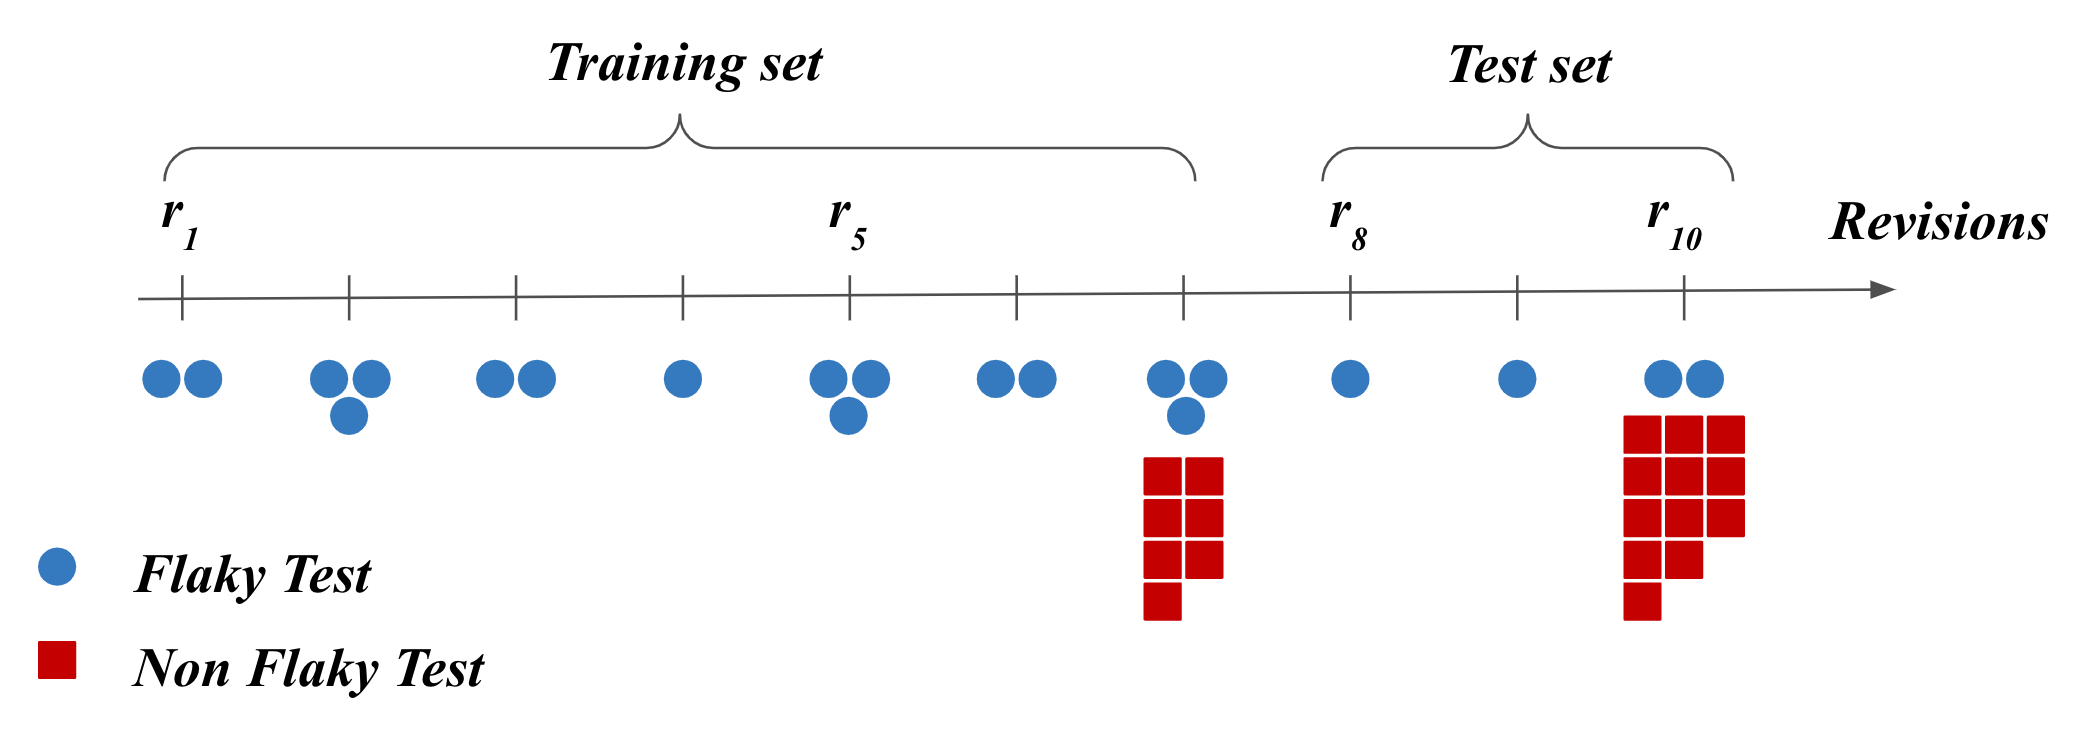
\includegraphics[width=0.8\textwidth]{figures/replication/fig1.png}
\caption{Time-sensitive validation}
\label{time-validation}
\end{figure}

To perform this comparison, we selected six projects from the DeFlaker dataset based on their numbers of flaky tests. 
These projects have at least 30 flaky tests, which we consider as a minimum necessary for training and testing a model. 
Table ~\ref{javaInfo} presents these projects with their numbers of flaky and non-flaky tests.
We also present the dates of the first and last flaky tests identified in these projects.
We split this dataset according to the two validation setups, then we build our prediction model, train it and contrast the results of both setups.

\begin{table}
\centering
\caption{Details about the Java projects used in our study}
\label{javaInfo}
 \begin{tabular}{l|r r r r r} 
 \toprule
 \textbf{Project} & \textbf{Earliest revision} & \textbf{Latest revision} &\textbf{ \#FT} & \textbf{\#NFT} \\ [0.25ex]
 \midrule
 achilles & 2015-10-30 & 2016-09-05 & 51 & 392 \\
 hbase & 2010-05-17 & 2010-06-21 & 98 & 120\\
 okhttp & 2014-03-06 & 2015-01-30 & 102 & 1178\\
 oozie & 2013-03-20 & 2013-05-31 & 1039 & 44 \\
 oryx & 2015-01-06 & 2015-02-27 & 38 & 286 \\ 
 togglz & 2016-01-23 & 2016-06-17 & 20 & 256 \\ 
 \bottomrule
\end{tabular}
\end{table}



\subsection{RQ2: Generalisation to other Programming Languages}
\subsubsection{Predicting flaky tests in Python}
Another goal of our study is to evaluate the generalisability of the original study to other programming languages.
For this purpose, we propose to assess the performance of flakiness prediction models on Python projects. 
We chose Python because it is the most popular language used in modern projects and it is commonly used for machine learning, web development, game development, and many other applications.

Python comes with its set of testing frameworks. 
We focus our study on Pytest\cite{pytestdocumentation}. Pytest is the equivalent of Junit for Python and enables developers to write tests for their programs. It is one of the main testing frameworks used in the open-source community and in the industry.
Pytest comes with its lot of features and plugins. Especially, a specific module to handle flaky tests can be used with Pytest: flaky\footnote{\url{https://pypi.org/project/flaky/}}.  
This module allows developers to annotate tests as flaky to automatically rerun them in case of failure. 
The developer can also configure the maximum amount of reruns to attempt and the minimum number of passes required. 
This annotation can be added to a test function or directly to the test class, giving its property to all of its tests. 
Figure~\ref{flaky-example} shows an example of a test marked as \emph{@flaky} taken from the Typed\_python project\footnote{\url{https://github.com/APrioriInvestments/typed\_python}}.

\begin{figure}[ht]
\centering
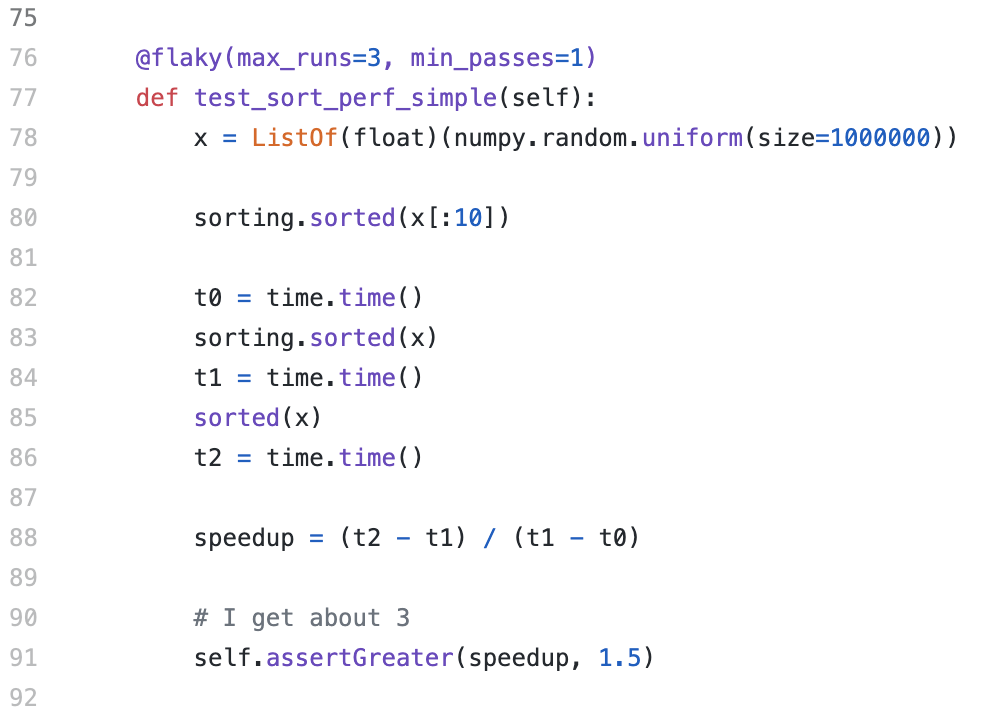
\includegraphics[width=0.8\textwidth]{figures/replication/flakyExample.png}
\caption{Example of a test labelled @flaky}
\label{flaky-example}
\end{figure}

We mined GitHub using the source-graph API\footnote{\url{https://sourcegraph.com/search}}, searching for Python projects containing the annotation \emph{@flaky}. 
This process yielded 110 projects with a total of 1,304 tests marked as flaky. 
Similarly to our first experimentation, we only select projects in which we have enough flaky tests to train and test a model, \ie 30 flaky tests.
This results in a dataset of 9 projects and 837 tests marked by developers as flaky.
Table ~\ref{pythonInfo} shows these projects with their number of flaky and non-flaky tests. 
Compared to the Java dataset, we were able to obtain more projects with more flaky tests for our study.
To the best of our knowledge, this is the first dataset of flaky tests in Python.

\begin{table}
\centering
\caption{Python projects used in our study}
\label{pythonInfo}
 \begin{tabular}{l|r r r r r} 
 \toprule
 \textbf{Project} & \textbf{SHA} & \textbf{\#FT }& \textbf{\#NFT}\\ [0.25ex]
 \midrule
 bokeh & ddc22b8 & 100 & 2505 \\
 cassandra-dtest & 8cb6bd2 & 72 & 4221 \\
 celery & 0833a27 & 54 & 2890 \\
 jira & 7fa3a45 & 131 & 59 \\
 pipenv & 8e64873 & 32 & 1612 \\
 python-amazon & 84c16f5 & 35 & 15 \\
 python-telegram-bot & 8e7c0d6 & 186 & 1382 \\
 spyder & 413c994 & 173 & 1086 \\
 typed-python & 96e7ebd & 54 & 6034 \\ 
 \bottomrule
\end{tabular}
\end{table}

It is worth noting that in this research question, we evaluate the performance of the model to predict flaky tests in a single revision. Therefore, we reuse the typical 80/20 dataset split as followed by Pinto \etal.  
That is, we are rather focusing on confirming that the approach works as well in Python and that a model can learn features differentiating tests labelled as \emph{@flaky} from the ones that are not. 
To extract these features, we use a bag of words representation of the test, as in Java. 
We also carefully remove the \emph{@flaky} annotations, as keeping it in the vocabulary would bias our model towards recognising this annotation rather than the code vocabulary.


\subsubsection{Predicting manifest flaky tests}
We perform further analysis in Python to assess the usefulness of a vocabulary-based model. 
Our objective is to evaluate the ability of a model to identify \textit{manifest} flaky tests based on training with tests labelled as flaky by developers. 
We consider as manifest flaky, every test for which we are able to observe non-deterministic behaviour dynamically.
This means that the test fails and passes at least once after several reruns.
To identify these manifest flaky tests, we reran 200 to 300 times the test suite of the three projects Bokeh, Celery and Python-telegram-bot. 
We run the test suites on a Mac machine with a 2,4 GHz 8-Core i9 processor and 32Gb of RAM.
The results of these reruns are presented in the table ~\ref{manifestStudy}.
The column \#@flaky shows the number of tests labelled as flaky in each project.
\begin{table}
\centering
\caption{Classifier performance for Python projects with manifest flaky tests}
\label{manifestStudy}
 \begin{tabular}{l|r r r r r} 
 \toprule
 \textbf{Project} & \textbf{\#reruns} & \textbf{\#@flaky} & \textbf{\#manifest FT}\\ [0.25ex]
 \midrule
 bokeh & 200 & 100 & 1 \\
 celery & 300 & 54 & 2 \\
 python-telegram-bot & 300 & 186 & 20 \\ 
 \bottomrule
\end{tabular}
\end{table}

We observe that despite the high number of reruns (800), only 23 tests have a flaky behaviour. This outcome is not surprising as flaky tests are, by nature, difficult to reproduce. To assess the model performance in detecting manifest flaky tests, we focus on the only project that has a reasonable amount of manifest flaky tests, namely Python-telegram-bot. We use the 20 manifest flaky tests found during our reruns as a test set, completed by 20 randomly selected tests that are not labelled as flaky. For the training set, we use the flaky and non-flaky tests minus the tests present in the test set. 

\subsection{RQ3: Extended Set of Features}
So far, the flakiness prediction is only based on features taken from the test code. 
However, flaky tests can be due to infrastructure or environmental issues (\eg lack of available resources in the CI, service or network unavailable, etc), to the test itself (\eg usage of dates, randomness, order dependency, etc), or to the CUT (\eg non-determinism, concurrency, etc). 
Notably, Luo~\etal~\cite{Luo2014} showed that 24\% of the fixes for flaky tests were applied to the CUT and that among them, 94\% fixed a bug in the CUT. 
Hence, it can be judicious to consider information from the CUT in flakiness prediction models. We propose to extend the original study by including the vocabulary of the CUT in test representation.

The main issue when considering the CUT is that computing the code coverage of each test during each revision would bring significant overheads. 
Besides, retrieving the exact code coverage dynamically goes against the goal of static prediction, which is to reduce dynamic costs.
To avoid this overhead, we propose a lightweight approach that relies on Information Retrieval (IR) to estimate the CUT. 

IR techniques have been used to solve different software engineering problems~\cite{Saha2014,Palomba2018,Azizi2018}. 
IR aims at quickly and automatically retrieving relevant information among a set of documents based on keywords taken from a user query. 
In our case, the query is the tokens of a test and the set of documents is the set of all functions (or methods) defined in the project. 
Our hypothesis is that functions from the CUT of a test are likely to use similar keywords (\ie variable names, API calls, etc) as the test. We are then looking for the most similar functions to our test function. To do so, we use a cosine similarity between a test case and a function from the CUT. Cosine similarity is defined with: 
\[cosSimilarity = \cos (Tc, Func) = \frac{Tc \cdot Func}{|Tc| |Func|}\]
where $Tc$ is the vector representing the test code and $Func$ is the vector representing the function code.
The result of a cosine similarity ranges from -1, meaning that the query - our test case - is completely different from the document - our function - to 1, where the query is perfectly similar to the document. 
In our case, we select the top three most similar functions for each test. 

\begin{algorithm}
\SetAlgoLined
\textbf{Inputs:}\\
Test[]\\
Function[]\\
\textbf{Outputs:}\\
TestWithCUT[]\\
\textbf{Procedure} \emph{CUT\_SELECTION(Test[], Function[])}\\
 \ForEach{ test T $ \in $ Test[]}{
   similarityMeasures[]\\
   Tvector = transform(T)\\
   \ForEach{function F $ \in $ Function[]}{
     fit($T+F$)\\
     Fvector = transform(F)\\
     cosTF = cosSimilarity(Tvector, Fvector)\\
     similarityMeasures.Append(cosTF)\\
   }
  similarityMeasures.Sort()\\
  similarityMeasures.Slice(0, 2)\\
  T.append(similarityMeasures)\\
  TestWithCUT.append(T)\\
 }
 \textbf{return} TestWithCUT[]
 \caption{Cost effective retrieval of the CUT}
 \label{algo}
\end{algorithm}

Algorithm~\ref{algo} describes the process of associating the CUT to each test. 
In order to compute the cosine similarity between the test and a function, we use the Text tokenisation utility class from the Keras library\footnote{\url{https://keras.io/api/preprocessing/text/}}. 
We first fit the \emph{Tokeniser} with the vocabulary from all tests and functions. 
Then, we transform the text of test and function bodies by creating a vector for each one of them of a length equal to the size of the vocabulary.
In this vector, each element represents the number of times a word appears in the body. 
After extracting the vectors, we compute the cosine similarity between the current test and all functions and store results. 
We finally filter to only keep functions that have a high score, \ie that they are the closest to the test. 
The body representation of the selected functions is used as a new set of features for the flakiness prediction model.
	% \section{FlakyCat}
\label{sec:flakycat-flakycat}

\begin{figure}[htbp]
\centering
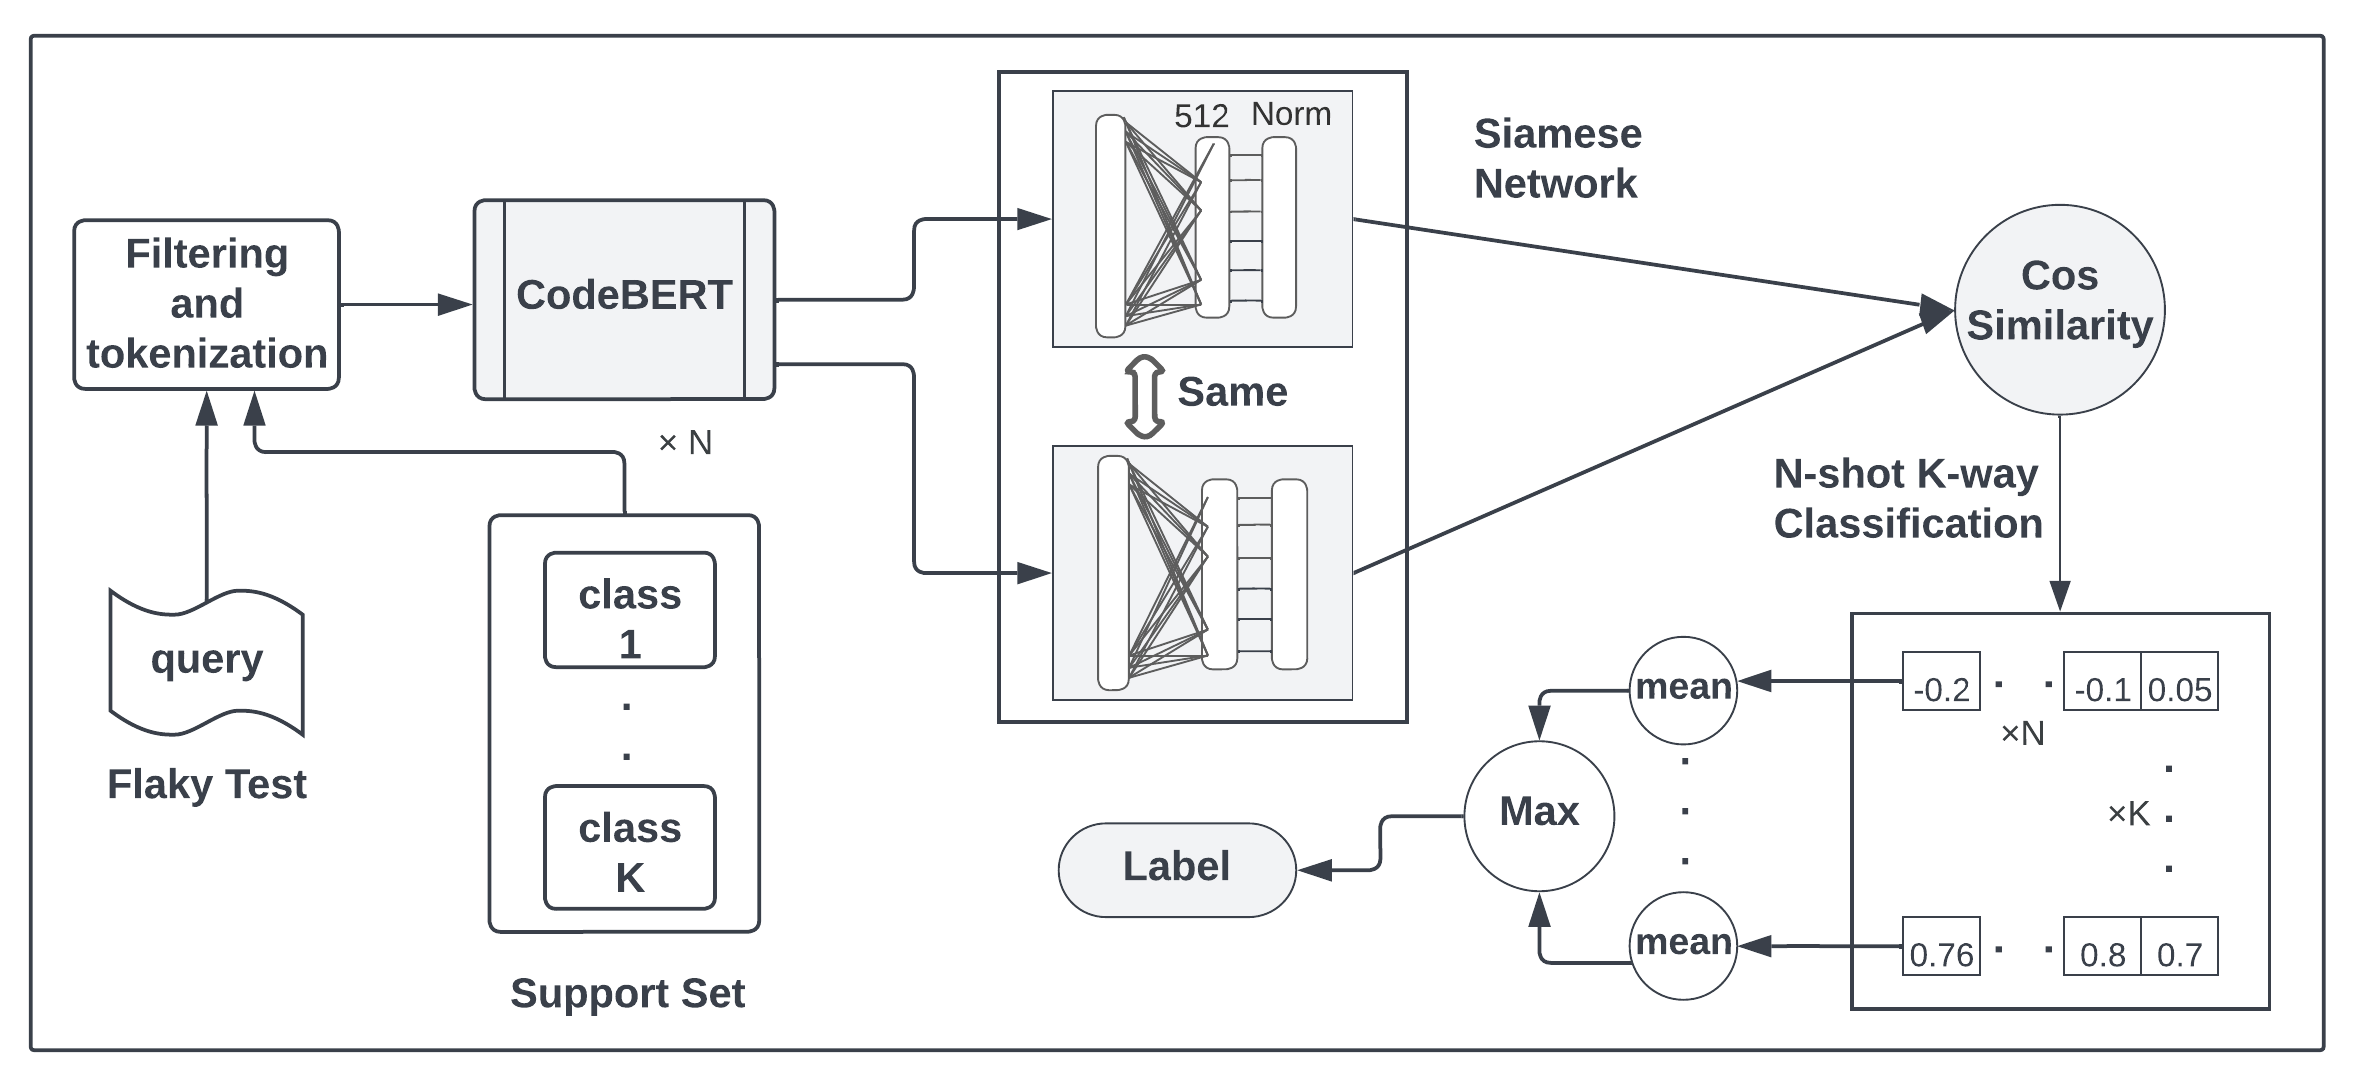
\includegraphics[width=0.8\textwidth,scale=1]{figures/flakycat/architecture.png}
\caption{An overview of FlakyCat, which combines the use of the pre-trained model CodeBERT, and Few Shot Learning based on the Siamese network.}
\label{fig:general_arch}
\end{figure}

In this section, we present the design and implementation of our approach.
Figure~\ref{fig:general_arch} presents an overview of the main steps of FlakyCat, code transformation and classification. 

\subsection{Step 1: Flaky test transformation}

\subsubsection{Scope} We rely on the test code to assign flaky tests to different categories.
Previous studies showed that flakiness finds its root causes in the test in more than 70\% of the cases\cite{Luo2014,Lam}. 
Hence, focusing on the test code allows us to capture the nature of flakiness while minimizing the overall cost of FlakyCat. 
Indeed, considering the code under test would require running the tests and collecting the coverage, which entails additional requirements and costs.



\subsubsection{Flaky test vectorization}
In order to perform a source code classification task, we first need to transform the code into a suitable representation that will be fed to the classification model. Among previous studies predicting flaky tests statically, two main approaches were used to transform code into vectors: using test smells~\cite{camara2021use,FlakeFlagger} and using code vocabulary \cite{pinto2020vocabulary,Haben2021,Camara2021VocabExtendedReplication}.
Both approaches seem promising, as different studies report high-performance models. As their encoding enables flaky test prediction, we believe they could also be used for flakiness category prediction, and we compare them with our approach. 


Recently, code embeddings from pre-trained language models were also considered for source code representation~\cite{fatima2021flakify,zhou2021assessing}. Pre-trained language models allow the encoding of code semantics and are intended for general-purpose tasks such as code completion, code search, and code summarization.
Considering these benefits, we use the pre-trained language model CodeBERT \cite{feng-etal-2020-codebert} to generate source code embeddings. 
CodeBERT can learn the syntax and semantics of the code and doesn't require any predefined features \cite{wan2022they}. Considering this aspect, we decide to rely on the CodeBERT test representation.

CodeBERT has been developed with a multi-layer transformer architecture~\cite{transformer} and trained on over six million pieces of code involving six programming languages (Java, Python, JavaScript, PHP, Ruby, and Go). 

To get the code representation using CodeBERT model, we first filter out extra spaces such as line breaks and tabs from the source code. In our case, we use each test method's source code as individual sequences. We then tokenise sequences by converting each token into IDs. Each sequence is passed to the CodeBERT model, which returns a vector representation. Figure~\ref{fig:using_codebert} illustrates this process.

Next, we explain the inputs and outputs of CodeBERT.

\paragraph{Inputs}
CodeBERT is able to process both source code and natural language, \eg comments and documentation. In our case, we did not exploit the possibility of using comments as the input length of CodeBERT is limited. Furthermore, comments can add noise since they represent unstructured text, possibly written by different developers, so we decided to solely rely on the code semantics. 
Hence, the given input to CodeBERT only considers code tokens, surrounded by two special tokens for boundaries. This is represented as follows: 
\begin{center}
 \([CLS], c1, c2, ..., cm, [SEP]. \)
\end{center}
Where \textit{Ci} is a sequence of code tokens, the special token [SEP] indicates the end of the sequence, and [CLS] is a special token placed in the beginning, whose final representation is considered as the representation of the whole sequence which we use for classification.


\paragraph{Outputs}

CodeBERT output includes two representations. The first one is the context matrix where each token is represented by a vector, and the second one is the CLS representation, having a size of 768, which is an aggregation of the context matrix and represents the whole sequence.
For the purpose of FlakyCat, we are interested in the CLS vector that represents the complete test code.

 
\begin{figure}[htbp]
\centering
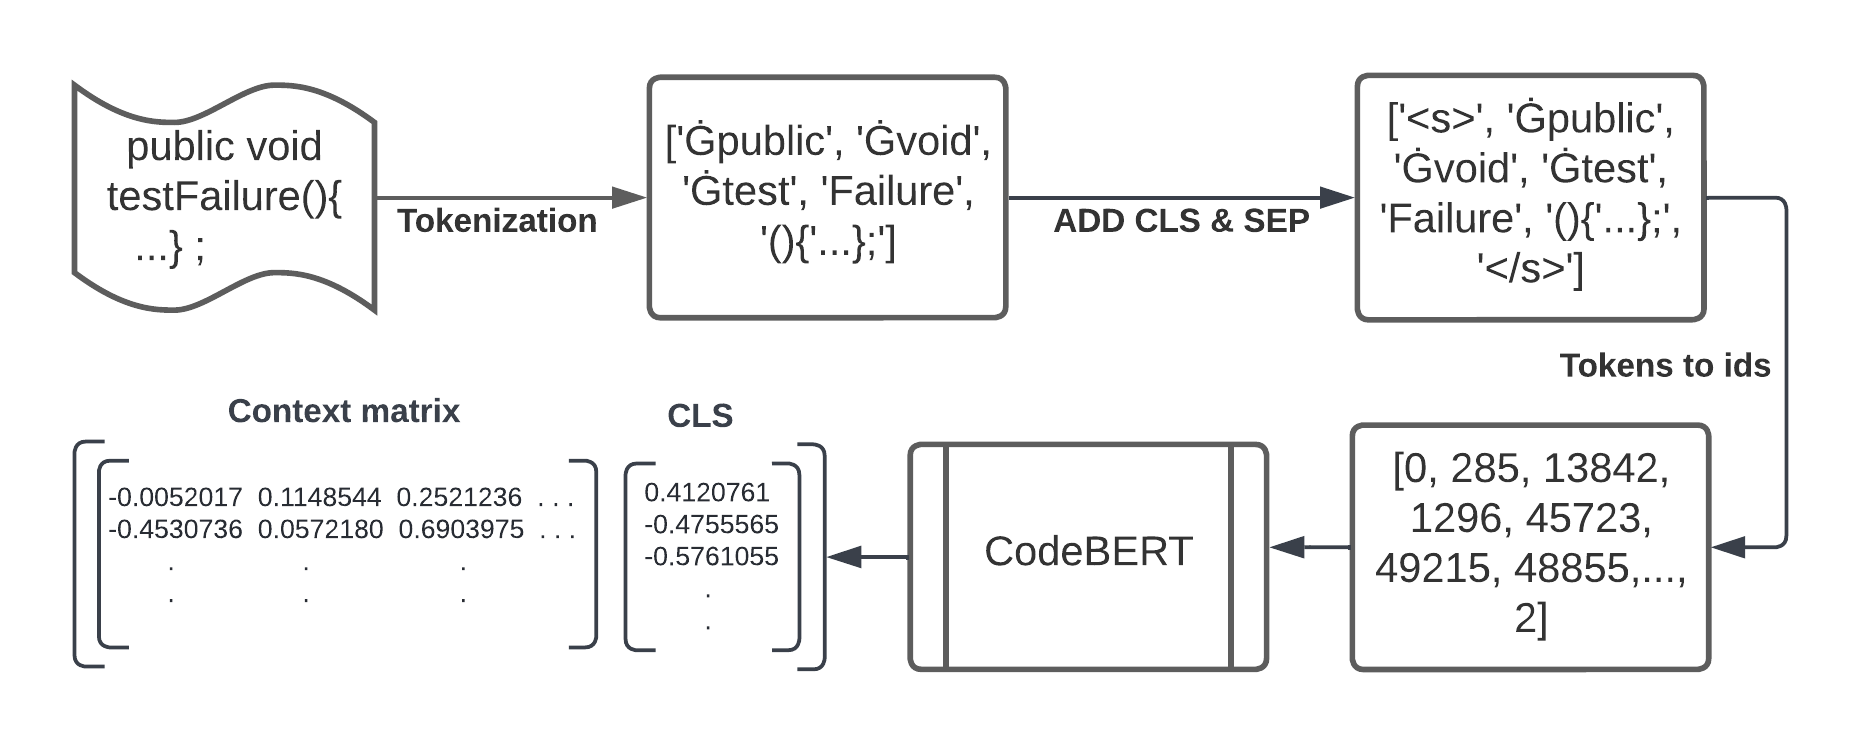
\includegraphics[width = 0.8\textwidth, scale=1]{figures/flakycat/codebert_transform.png}
\caption{The process of converting the source code of each test case to a vector using CodeBERT, going through tokenization, then converting to IDs and applying the CodeBERT model to get the representation (CLS vector). Ǵ represent spaces, $<s>$ used for CLS, and $</s>$ for SEP. }
\label{fig:using_codebert}
\end{figure}

\subsection{Step 2: Flaky test categorization}

\subsubsection{Classification process}

Unlike traditional machine learning classifiers that attempt to learn how to match an input $x$ to a probability $y$ by training the model in a large training dataset and then generalizing to unseen examples, Few-Shot Learning (FSL) classifiers learn what makes the elements similar or belonging to the same class from only a few data. Facing the scarcity of data on flaky tests, selecting an FSL classifier seems then to be a promising choice. 


In FSL, we call the item we want to classify a \textit{query}, and the \textit{support set} is a small set of data containing few examples for each class used to help the model to make classifications based on similarity as shown in Figure~\ref{fig:general_arch}.
To classify flaky tests according to their flakiness category, we compute the similarity between the query and all examples of each flakiness category in our Support Set and assign the label having the maximum similarity with the query. This classification is obviously performed in a space where all elements of the same class are similar or close to each other. This is achieved by a model called \textit{Siamese network}. Its task is to transform the data and project it into a space where all the elements of a same class are close to each other, and then to classify the elements by computing their similarity.



The Siamese network has knowledge of the similarity of elements of the same class. It processes two vectors in input and applies transformations that allow minimizing the distance between the two vectors if they share similar characteristics. Figure~\ref{fig:before_after} shows an example of the visualization of flaky test vectors before and after the Siamese network is applied. Since CodeBERT has no knowledge of the characteristics of flaky tests and only generates a general representation of the source code, the vectors produced are all similar.
However, the Siamese networks learn which characteristics in these vectors are shared by tests of the same class, and thus allow to project vectors into a space that groups tests of the same flakiness category. After this step, it becomes possible to classify them using a similarity computation.

\begin{figure}[htbp]
\centering
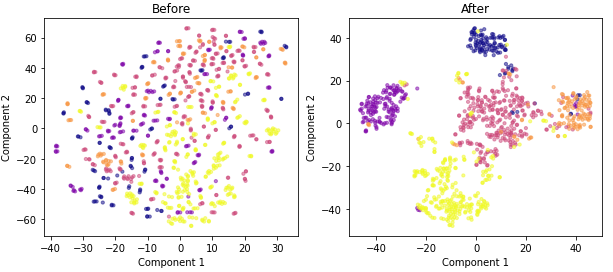
\includegraphics[width = 0.8\textwidth, scale=1]{figures/flakycat/before_after.PNG}
\caption{Visualization of our data before and after training of the Siamese network with the triplet loss, which brings together the elements of the same class.}
\label{fig:before_after}
\end{figure}
\vspace{3mm}

\subsubsection{Model training}


Siamese networks have two identical sub-networks, each sub-network processes the input vector and performs transformations.
Both sub-networks are trained by calculating the similarity between the two inputs and using the similarity difference as a loss function.
Accordingly, the weights are adjusted to have a high similarity if the inputs belong to the same class. For the architecture of the sub-networks, we used a dense layer of 512 neurons and a normalization layer as shown in Figure~\ref{fig:general_arch}.
We also performed a linear transformation to keep relations learnt by CodeBERT using the attention mechanism introduced in the transformer architecture \cite{attention}. 
This model is trained using a Triplet Loss function, based on the calculation of similarity difference.

Let the Anchor $A$ be the reference input (it can be any input), the positive example $P$ is an input that has the same class as the Anchor, the negative example $N$ is an input that has a different class than the Anchor, $s()$ is the cosine similarity function, and $m$ is a fixed margin. The idea behind the Triplet Loss function is that we maximize the similarity between $A$ and $P$, and minimize the similarity between $A$ and $N$, so ideally $s(A, P)$ is large and $s(A, N)$ is small. The formula for this loss function is: 

\vspace{3mm}
\begin{center}
\( Loss = max(s(A, N) - s(A, P) + m, 0) \)
\end{center}
\vspace{3mm}

$m$ is an additional margin as we do not want $s(A, P)$ to be very close to $s(A, N)$, which would lead to a zero loss. 

To train the Siamese network with the triplet loss, we give as input batches of pairs with the same classes, and any other pair of a different class can be used as a negative example. We select the closest negative example to the anchor, such as $s(A,  N)$ $\simeq$ $s(A, P)$, which generates the largest loss and constitutes a challenge for model learning. 
	% \section{Chromium}
\label{sec:chromium-chromium}


\subsection{Overview}

% General Information about Chromium
Started in 2008, with more than 2,000 contributors and 25 million lines of code, the Chromium web browser is one of the biggest open-source projects currently existing. Google is one of the main maintainers, but other companies and contributors are also taking part in its development.

% LuCI hierarchy
Chromium relies on \textit{LuCI} as a CI platform~\cite{onlineChromiumGithub}.
It uses more than 900 parallelized builders, each one of them used to build Chromium with different settings (\eg different compilers, instrumented versions for memory error detection, fuzzing, etc) and to target different operating systems (\eg Android, Mac OS, Linux, and Windows). 
% Additionally, some builders are only responsible for running test suites. 
Each builder is responsible for a list of builds triggered by commits made to the project. If a builder is already busy, a scheduler creates a queue of commits waiting to be processed. This means that more than one change can be included in a single build execution if the development pace is faster than what the builders can process. Within a build, we find details about build properties, start and end times, status (\ie pending, success or failure), a listing of the steps and links to the logs. 

% Testing infrastructure
At the beginning of the project, building and testing were sequential. Builders used to compile the project and zip the results to builders responsible for tests. Testing was taking a lot of time, slowing developers' productivity and testing Chromium on several platforms was not conceivable. A swarming infrastructure was then introduced in order to scale according to the Chromium development team's productivity, to keep getting the test results as fast as possible and independently from the number of tests to run or the number of platforms to test. Currently, a fleet of 14,000  build bots runs tasks in parallel. This setup helps to run tests with low latency and handle hundreds of commits per day~\cite{TheChromiumProjects}.

% Figure Decision tree
\begin{figure}[ht]
\centering
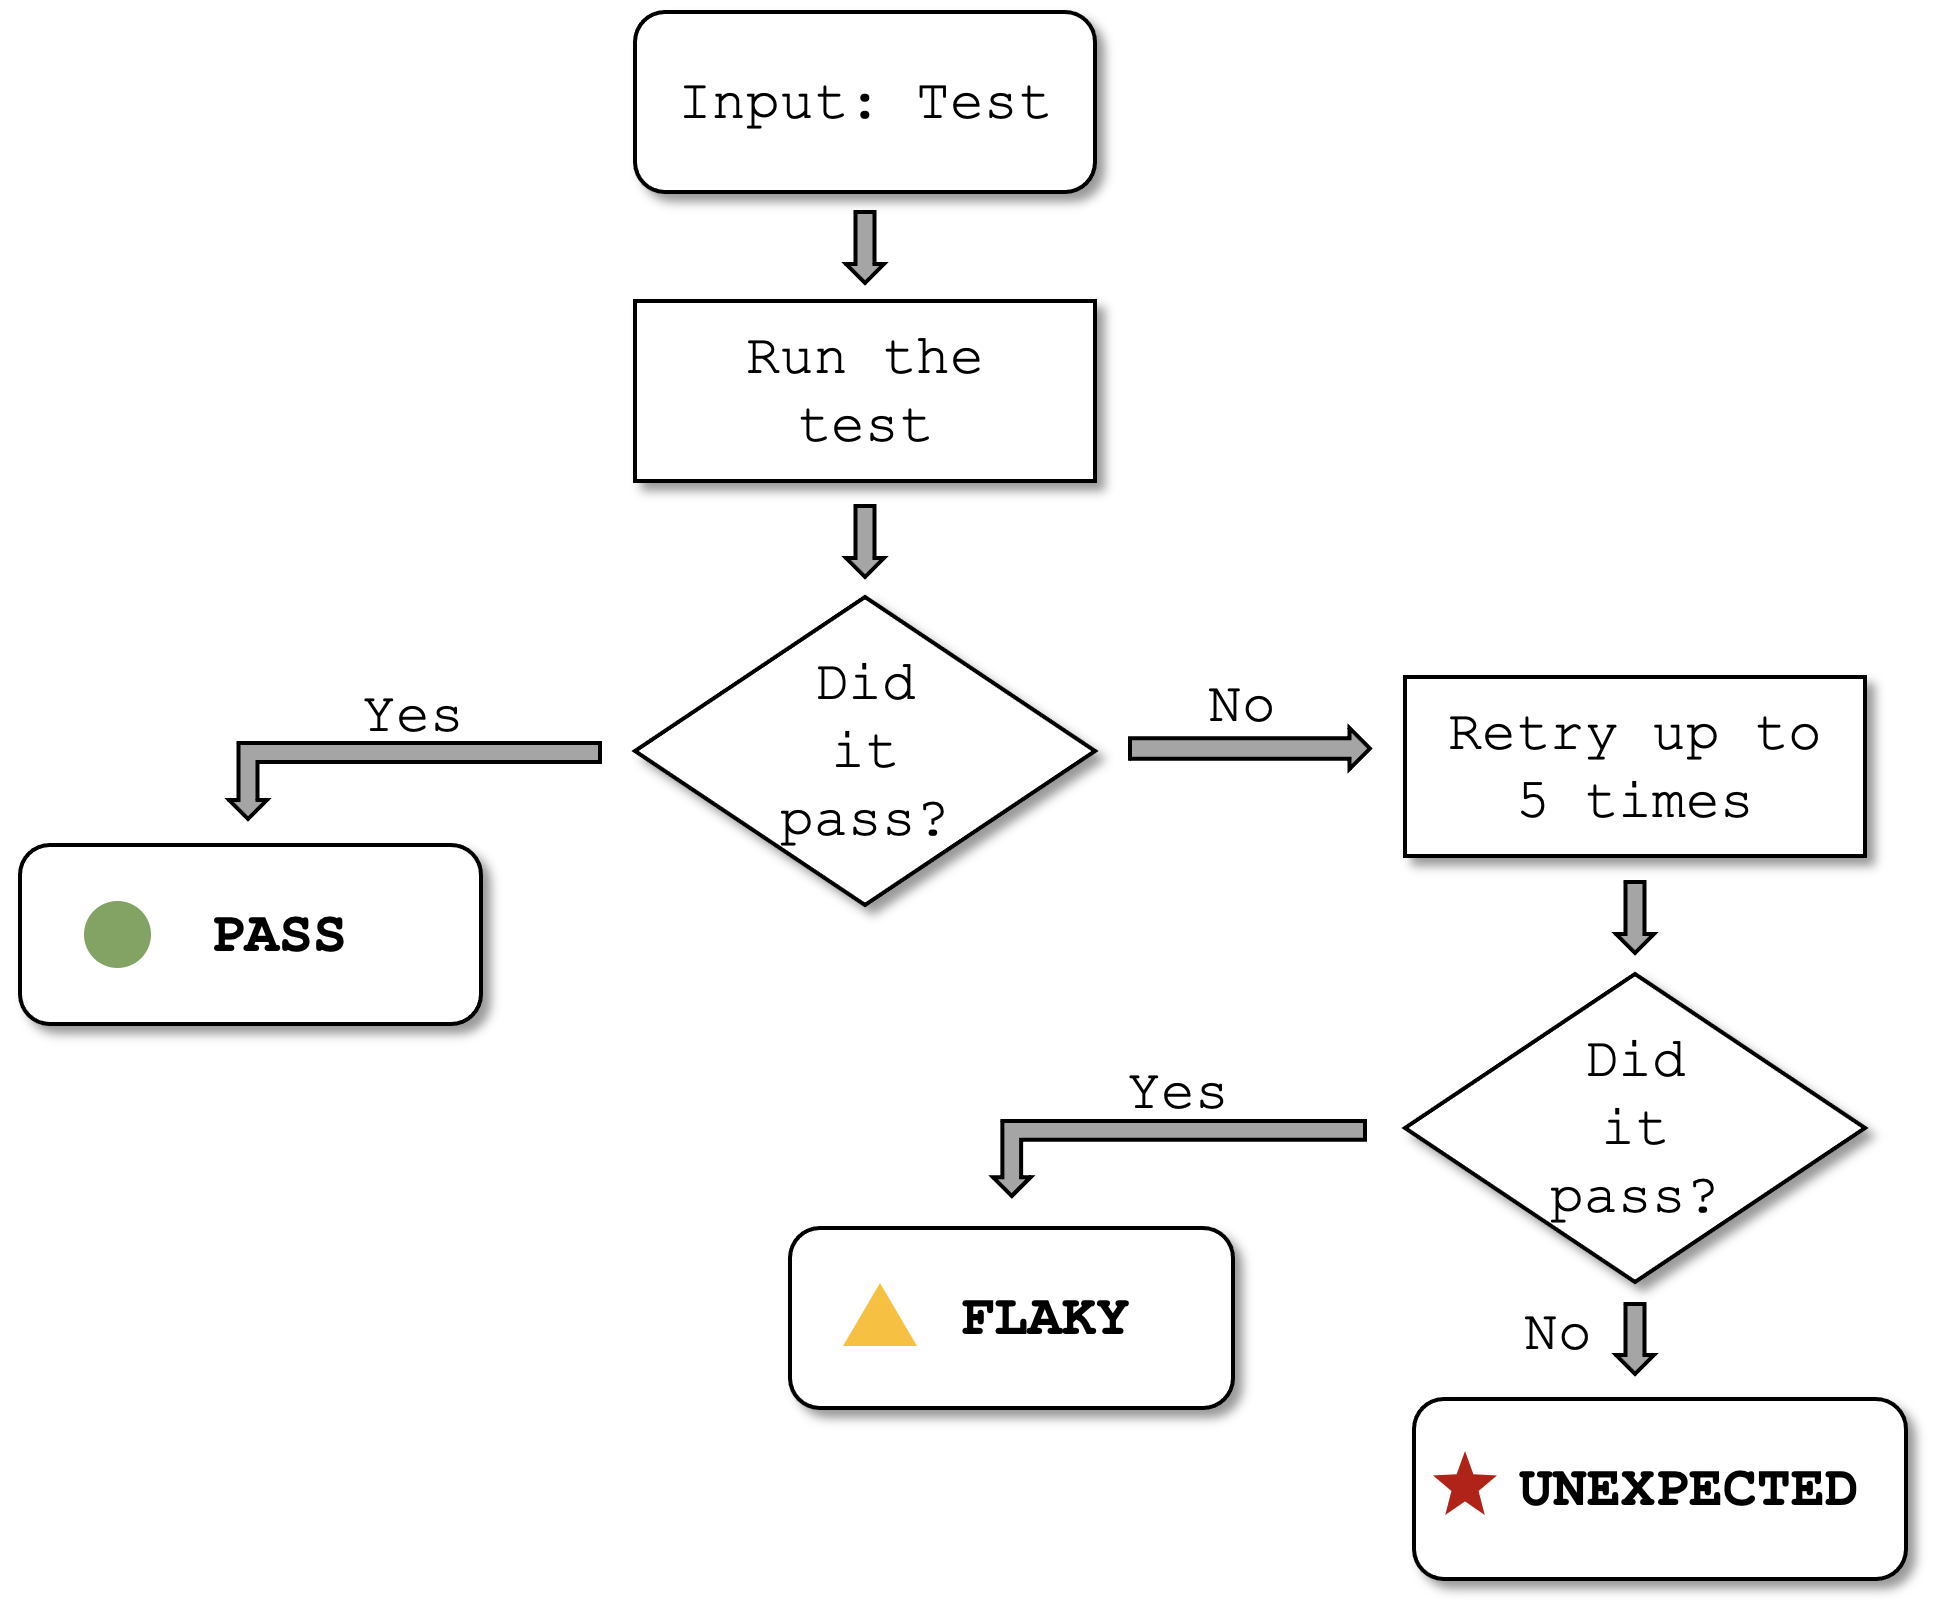
\includegraphics[width=0.8\textwidth]{figures/chromium/gui_process_final.png}
\vspace{-1.0em}
\caption{Decision tree representing how test outcomes are determined in a build by the Chromium CI. 
\includegraphics[scale=0.2]{figures/chromium/pass.png} PASS depicts successful tests, 
\includegraphics[scale=0.2]{figures/chromium/flaky.png} FLAKY depicts tests that passed after failing at least once, while 
\includegraphics[scale=0.2]{figures/chromium/fail.png} UNEXPECTED depicts tests that persistently failed.}
\label{fig:decision-tree}
\end{figure}

% Information about tests
In this study, we focus on testers, \ie builders only responsible for running tests. They do not compile the project: when triggered, they simply extract the build from their corresponding builder and run tests on this version. At the time of writing, we found 47 testers running Chromium test suites on distinct operating systems versions. About 200,000 tests are divided into different test suites, the biggest ones being \textit{blink\_web\_tests} (testing the rendering engine) and \textit{base\_unittests} with more than 60,000 tests each.

% Build results
For each build performed by any tester, we have access to information about test results. Figure~\ref{fig:decision-tree} illustrates the decision process followed by LuCI to determine a test outcome in a specific build. A test is labelled as \textit{pass} when it successfully passed after one execution. In case of a failure, LuCI automatically reruns the test up to 5 times. If all reruns fail, the test is labelled as \textit{unexpected} and will trigger a build failure. In the remaining, we will be referring to \textit{unexpected} tests as \textit{fault-revealing tests}. If a test passes after having one or more failed executions during the same build, it is labelled as \textit{flaky} and will not prevent the build from passing. 


\subsection{Example of a flaky test}

%In this subsection, we discuss an example of a flaky test. By doing so, we seek to give a clearer idea of what Chromium's tests may look like. Furthermore, we show the pieces of information that can be extracted from the tests and used for flakiness detection.

% Figure Decision tree
\begin{figure}[ht]
\centering
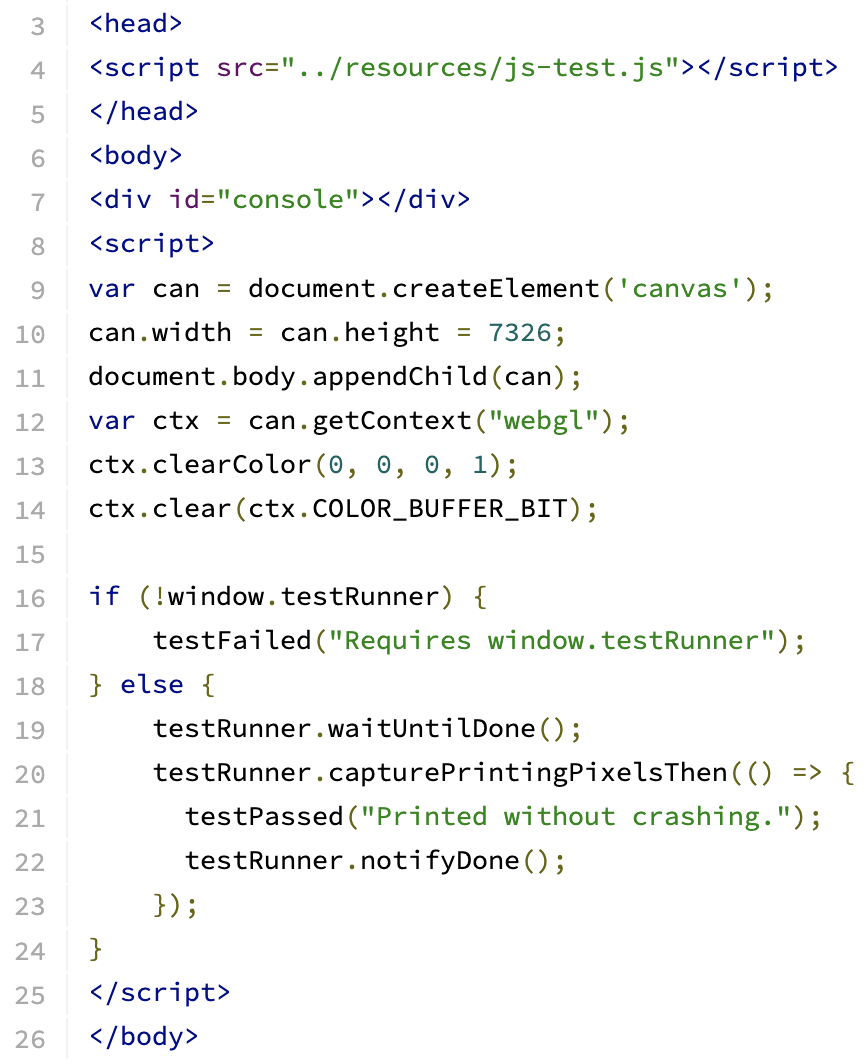
\includegraphics[width=0.8\textwidth]{figures/chromium/flakyTestExample.png}
%\vspace{-1.0em}
\caption{An example of a flaky test caused by a timeout. The test consists of an HTML file \texttt{printing/webgl-oversized-printing.html}, build 119,039 of the Linux Tester. The call to \textsc{waitUntildone()} on line 19 is likely the reason for the failure.}
\label{fig:example}
%\vspace{-0.5em}
\end{figure}

Figure~\ref{fig:example} shows a flaky test found in build 119,039\footnote{https://ci.chromium.org/ui/p/chromium/builders/ci/Linux\%20Tests/119039/} of the Linux Tester. This test, \texttt{printing/webgl-oversized-printing.html}, ensures that no crash happens on the main thread of the rendering process when using the system. Unfortunately, on its first execution, the test failed after 31 seconds. The run status indicates that a \textsc{TIMEOUT} happened. On the second execution, the test passed after 15 seconds and thus was labelled as flaky. In this case, an issue has been opened in Chromium's bug tracking system.\footnote{https://bugs.chromium.org/p/chromium/issues/detail?id=1393294} Developers state that \textit{"this test makes a huge memory allocation in the GPU process which intermittently causes OOM and a GPU process crash"}.

\textsc{Timeout} is a run status that intuitively leads to possible flakiness, as we can easily think of other executions of the same test being completed before reaching the time limit. In addition to this feature, we can also look for hints of flakiness in the source code. As with many UI tests in Chromium, this one is handled by \texttt{testRunner}: a test harness in charge of their automatic executions. We can see the \texttt{testRunner} making a call to \texttt{waitUntilDone()} on line 19. Vocabulary about waits is common in Chromium's web tests. This keyword, for example, could potentially be leveraged by flakiness detectors to classify tests or failures.


% Former place for fig 2: decision tree


	\chapter{Pinpointing Classes Responsible for Test Flakiness}
\label{chap:sherloc}

\setcounter{minitocdepth}{1}
\justifying
\textit{Still with the goal of helping to debug flakiness, we present in this chapter a new approach to locate the source of flakiness when it originates from the code under test. This represents a specific but critical case as the cause of non-determinism lies in the program itself. The approach leverages Spectrum-Based Fault Localisation techniques, code and change metrics and ensemble learning to rank classes the most likely to be responsible for flakiness.\\
}

\chapterPage{This chapter is based on the work published in the following paper:\\
\begin{itemize}
\vspace{-2mm}
\item \fullcite{habchiPinpointing}
\end{itemize}}

\section{Introduction}
\label{sec:sherloc-introduction}

Regression testing is a key component of continuous integration (CI) that checks whether code changes integrate well in the codebase without breaking any existing functionality. To this end, it is assumed that failing tests indicate the presence of faults, introduced by the latest changes. However, some tests break this assumption by failing for reasons other than faults, as for instance,  they exhibit non-deterministic behaviour, thereby sending confusing signals to developers. Such tests are usually called \textit{flaky tests}.

Academic and industrial reports have emphasised the adverse effects of test flakiness in software development. Specifically, Google reported that 16\% of their tests manifested some level of flakiness, while more than 90\% of their test transitions, either to failing or passing, were due to flakiness~\cite{LeongSPTM19}. 
As the \textit{de facto} approach for detecting flaky tests is to rerun them \cite{Habchi2022Qualitative, gruber2022survey}, detecting large numbers of flaky tests can be time- and resource-consuming. Indeed, Google reports that between 2 to 16\% of their CI resources are dedicated in rerunning flaky tests~\cite{Micco2017}. It is noted  that other companies, like Microsoft~\cite{Lam2020b},  Spotify~\cite{FlakinessSpotify} and Mozilla~\cite{Rahman2018}, also report similar issues when dealing with test flakiness. 

Perhaps more importantly, test flakiness affects team productivity and software quality \cite{Habchi2022Qualitative}. This is because flaky failures interrupt the CI and make developers waste time in investigating false issues~\cite{GTAC2016,Eck2019,LeongSPTM19,Habchi2022Qualitative}. Additionally, the accrual of flaky tests breaks the trust in regression testing, leading developers to disregard legitimate failure signals believing them to be false~\cite{Habchi2022Qualitative, gruber2022survey}. This situation often results in faults slipping into production systems~\cite{Rahman2018}. Moreover, code quality is often linked with the level of flakiness incurred \cite{Habchi2022Qualitative} and thus, developers need to know where it comes from and understand the causes of flakiness to avoid introducing and spreading it. 

Given the adverse effects of test flakiness, engineers and researchers aim at developing 

detection techniques that can predict whether a test is potentially flaky. These approaches rely on a number of runs and re-runs, such as \textsc{iDFlakies}~\cite{Lam2019iDFlakies} and \textsc{Shaker}~\cite{Silva2020}, coverage analysis like \textsc{DeFlaker}~\cite{Bell2018}, or static and dynamic test features~\cite{FlakeFlagger,Haben2021,Pinto2020,Dong2021,Camara2021VocabExtendedReplication,camara2021use,fatima2021flakify}.  
Evaluated on open-source projects, these approaches showed promising detection accuracy and considerably decreased the amount of time and resources needed to detect flaky tests. 

Although flakiness detection methods are important, alone, they cannot reduce the prevalence of test flakiness. This is because on the one hand there are only partial approaches to  the problem,  such as  \textsc{iFixFlakies}~\cite{Shi2019iFix} and \textsc{Flex}~\cite{FLEX} that are only applicable to specific cases, and the inherent difficulties in isolating/controlling the flakiness causes on the other. For instance, \textsc{iFixFlakies}~\cite{Shi2019iFix} fixes order-dependent tests by identifying helper statements in other tests, whereas \textsc{Flex}~\cite{FLEX} identifies  assertion bounds that minimise flakiness stemming from algorithmic randomness. At the same time, many prevalent categories of flakiness, \eg  Asynchronous Waits and Concurrency~\cite{Gruber2021,romano2021empirical,Luo2014, Eck2019}, remain unaddressed by fixing approaches. This is mainly due to the difficulty of identifying  and controlling the cause of flakiness~\cite{Eck2019}. 

Flakiness root cause localisation is both important and difficult. It is important since it allows developers to understand the sources of flakiness, hence enabling better control of non-determinism. It is also difficult because of the difficulty to reproduce failures, the diversity in potential issues, \eg time and network, and the large scope of potential culprits, \eg the tests, the code under test (CUT), and the infrastructure~\cite{Gruber2021}. Consequently, practitioners struggle to identify the causes of non-determinism in their codebases that trigger flakiness and consider this step as the main challenge in automating flakiness mitigation strategies~\cite{Eck2019}. 

In this paper, we address this challenge by re-targeting Fault Localisation (FL) techniques in order to help identify components (program classes in particular) that are responsible for the non-deterministic behaviour of flaky tests. For the sake of simplicity, we refer to these classes as \textit{flaky classes}. Such techniques can be useful to support the analysis  of codebases and of flaky tests. Thus, given a failure, either known as flaky or unknown, engineers can rely on localisation methods to investigate the specific scenario (condition) that causes the test transition. Additionally, flakiness localisation techniques can help with code comprehension and make engineers aware of code areas linked with flaky behaviour, assisting them in both development and testing tasks. 

In view of this, we investigate the appropriateness of a variety of fault localisation methods, such as Spectrum-Based Fault Localisation (SBFL), change history metrics, and static code metrics in identifying flaky classes. 
Our study aims to answer the following four research questions:

\begin{itemize}[label={}]
    \item \textbf{\textsc{RQ1:}} \emph{Are SBFL-based approaches effective in identifying flaky classes?}
    \item \textbf{\textsc{RQ2:}} \emph{How do code and change metrics contribute to the identification of flaky classes?}
    \item \textbf{\textsc{RQ3:}} \emph{How can ensemble learning improve the identification of flaky classes?}
    \item \textbf{\textsc{RQ4:}} \emph{How does an SBFL-based approach perform for different flakiness categories?}
\end{itemize}

To answer these questions, we analyse five Open Source projects where test flakiness has been fixed during the project evolution. Our analysis shows that: 
\begin{itemize}
    \item An ensemble of models based on SBFL, change, and size metrics, yields the best results, with 61\% of flaky classes in the top 10 and 26\% of them at the top. 
    %This method also lowers the average effort wasted by developers to 3.5.
    This method also reduces the average effort wasted by developers to 19\% of the effort spent when inspecting all classes covered by the flaky test.
    \item The ensemble method is effective for major flakiness categories. Concurrency and Asynchronous Waits are identified effectively, with 38\% and 30\% of their flaky classes ranked at the top, respectively.
\end{itemize}

To facilitate the reproducibility of this study, we provide all used scripts,  the set of collected flaky classes, and detailed results in a comprehensive package\footnote{\url{https://github.com/serval-uni-lu/sherlock.replication}}.

\section{Data Collection}
\label{sec:sherloc-data}

The objective of our study is to assess the effectiveness of FL techniques in identifying flaky classes.
To achieve this, we need a set of flaky tests for which the responsible classes are already known. 
For this, we rely on flakiness-fixing commits as they provide information about classes that were modified as part of the fix.
Our assumption is that such classes are, at least, part of the root cause. % JJ-to-do: citation (to show that this is also a common pratice in FL? 
To collect flaky classes, we followed a four-step process.

\paragraph{Search} 
This step aims to identify Java projects containing the highest number of flakiness-fixing commits. For this, we relied on two sets of projects to consider. 
We built the first set by using the SEART GitHub Search Engine~\cite{githubsearch}. Out of the 81,180 available Java projects, we selected the top 200 projects for each of those criteria: number of commits, contributors, stars, releases, issues, and files. This sorting was made with the aim of finding the bigger and more complex projects, thus maximising our chance to find flakiness-fixing commits. 
Keeping only unique projects in those sets, we ended up with a first list of 902 projects. As a second set, we use the 187 projects available in the \textsc{iDFlakies} dataset~\cite{Lam2019iDFlakies}. 
For each of the 1,089 projects, 902 from the first and 187 from the second set, we query the GitHub API looking for commits with messages containing the keyword \textit{flaky}. This led to the identification of 16,501 commits.
We look further into whether these commits are truly suitable for our purpose through the following processes. 

\newcommand\mch[2]{\multicolumn{1}{>{\centering\arraybackslash}b{#1}}{#2}}
% TODO: I don't really know if it makes sense to show #Flaky tests because:
% When we don't know which particular test was flaky we over approximate it by
% marking all test from the test class as flaky.


\begin{table}[t]
\vspace{-0.5em}
\caption{Collected Data. \textit{ffc:} number of flakiness-fixing commits. \textit{all:} number of commits in the project.
\vspace{-0.5em}
\centering}
\centering
\label{tab:SD-info}
\scalebox{0.8}{
\begin{tabular}{l|cc|cc|cc}
\toprule
%Project & \# Commits & \# Flaky Tests & \multicolumn{3}{c|}{\# Tests} & \multicolumn{3}{c}{\# Classes} \\
\textbf{Proj. } & \multicolumn{2}{c|}{\textbf{\#Commits}} & \multicolumn{2}{c|}{\textbf{\#Tests}} & \multicolumn{2}{c}{\textbf{\#Classes}} \\
 & ffc & all &  min - max & avg & min -- max & avg \\
\midrule
Hbase & 8 & 18,990 & 138 - 2,089 & 1,113 & 734 -- 1366 & 1053.4 \\
Ignite & 14 & 27,903 & 15 - 1,018 & 174 & 72 -- 1767 & 1262.3 \\
Pulsar & 10 & 8,516 & 194 - 1,326 & 626 & 171 -- 422 & 259.7 \\
Alluxio & 3 & 32,560 & 315 - 694 & 473 & 131 -- 817 & 360.3 \\
Neo4j & 3 & 71,824 &  21 - 5,782 & 2,139 & 40 -- 1663 & 581.3 \\
\midrule
Total & 38 &  &  15 - 5,782 & 905 & 40 -- 1767 & 820.2 \\
\bottomrule
\end{tabular}
}
\vspace{-5mm}
\end{table}


%\begin{table}[t]
%\begin{center}
%\caption{Collected Data. \textit{ffc:} number of flakiness-fixing commits. \textit{all:} number of commits in the project.
%\centering}
%\centering
%\label{tab:SD-info}
%\scalebox{0.8}{
%\begin{tabular}{l|cc|cc|cc|cc}
%\toprule
%Project & \# Commits & \# Flaky Tests & \multicolumn{3}{c|}{\# Tests} & \multicolumn{3}{c}{\# Classes} \\
%\textbf{Proj. } & \multicolumn{2}{c|}{\textbf{\#Commits}} & \multicolumn{2}{c|}{\textbf{\#Tests}} & \multicolumn{2}{c}{\textbf{\#Classes}} & \multicolumn{2}{c}{\textbf{\#Cov.Classes}} \\
% & ffc & all &  min - max & avg & min -- max & avg & min -- max & avg \\
%\midrule
%Hbase & 8 & 18,990 & 138 - 2,089 & 1,113 & 734 -- 1366 & 1053.4 & 2x -- 387x & 243x \\
%Ignite & 14 & 27,903 & 15 - 1,018 & 174 & 72 -- 1767 & 1262.3 & 24x -- 716x & 463x \\
%Pulsar & 10 & 8,516 & 194 - 1,326 & 626 & 171 -- 422 & 26059.7 & 2x -- 120x & 59x \\
%Alluxio & 3 & 32,560 & 315 - 694 & 473 & 131 -- 817 & 360.3 & 19x -- 90x & 65x \\
%Neo4j & 3 & 71,824 &  21 - 5,782 & 2,139 & 40 -- 1663 & 581.3 & 1x -- 480x & 163x \\
%\midrule
%Total & 38 &  &  15 - 5,782 & 905 & 40 -- 1767 & 820.2 & x -- x & x \\
%\bottomrule
%\end{tabular}
%}
%\end{center}
%\vspace{-5mm}
%\end{table}

\paragraph{Inspection}
The objective of this step is to filter commits that do not provide a clear indication about the flaky class. Hence, we look for flakiness-fixing commits containing any of the following keywords: \textit{fix, repair, solve, correct, patch, prevent}. Then, we analyse each commit and keep the ones that:
\begin{itemize}[wide=0pt,noitemsep,topsep=0pt]
    \item The fix affects the code under test 
    (not only the test itself);
    \item The changes are atomic enough (\ie containing only relevant changes) allowing us to discern the flaky class(es). 
\end{itemize}

This led to the selection of 85 commits from five projects. We further discarded 22 commits for which the flaky tests or commit were not retrievable (\eg rejected pull request), leaving 63 commits in the end. 


\paragraph{Test execution}
This step aims to select commits that are usable in our evaluation.
Our first question inspects the effectiveness of SBFL, a technique that requires a coverage matrix indicating the classes covered by each test.
Hence, for a commit to be usable in our analysis, its test suite should be runnable allowing us to extract the coverage matrix.
To ensure this, we used  \textsc{GZoltar}\footnote{\url{https://github.com/GZoltar/gzoltar/blob/master/com.gzoltar.ant/}}, a Maven plugin that allows collecting coverage information for each commit.
% We found that for 44 commits our tool was not able to provide consistent results. In particular, 15 commits results were discarded because (i) the patches provided did not change the program behaviour (e.g. console prints, comments, build file modification) 2) only the test was patched (thus not addressing the flakiness behaviour ) 3) the commit was not included in the original repository (e.g. fork).
% The other vast majority (i.e. 15) of the commits results were discarded as the flaky test could not be identified. 
% Finally, for the remaining 14 commits , the tool was not able to provide any results due mainly to incompatible java version.
For 11 commits, we were unable to run \textsc{GZoltar} due to an incompatible Java version. We also found that the flakiness patches were irrelevant in 10 commits.
For instance, some commits were fixing modules in other programming languages or modifying non-source code files.
% Need to check!
Lastly, we filtered out four additional commits since the reported flaky failures were not \textit{flaky test failures}.
Consequently, %this step resulted in 38 commits from 5 projects by dropping 
we dropped 25 commits in addition. Table~\ref{tab:SD-info} summarises the retained projects.
The complete list of flakiness-fixing commits is available in our replication package. 

\paragraph{Extraction}
For each collected flakiness-fixing commit, we retrieve the source code, the test suite, the fixed flaky test, and the flaky class. To retrieve the flaky classes, two authors manually analysed the commit diff and message to identify them.
Overall, the identification was obvious since we selected atomic commits beforehand.
Hence, there were no disagreements between the authors at this step.
The identified classes are considered the ground truth of our study. 


\section{Study Design}
\label{sec:sherloc-design}

\subsection{RQ1: Effectiveness}\label{sub:rq1_effectiveness}
\subsubsection{Motivation}\label{subsub:rq1_motivation}

The objective of our study is to investigate the usability of well-founded FL techniques to help in mitigating flaky tests.
The literature on FL proposes a wide variety of categories such as ML-based techniques~\cite{Lou:2021:fse,DeepFL,briand2007}, mutation-based techniques~\cite{Papadakis:2015sf,Hong:2015db}, and qualitative reasoning-based techniques~\cite{perez2018leveraging}.
Nonetheless, spectrum-based fault localisation remains one of the most distinguished FL categories thanks to its effectiveness and simplicity~\cite{wong2016survey}.

SBFL requires only the test coverage matrix to compute the likelihood for a code entity to include the root cause of an observed test failure. 
The main assumption of SBFL is that code entities covered by more failing tests and fewer passing tests are more suspicious than those less covered by failing tests and more by passing tests~\cite{Renieres2003}.
This assumption can be revised to identify the root causes of flaky tests instead of bugs.
In particular, if we separate tests into two groups: \textit{flaky} and \textit{stable}, instead of \textit{failing} and \textit{passing}, we can leverage the coverage matrix to rank classes based on their correlation with flaky tests. 
In this case, the assumption would be that classes covered by more flaky tests and fewer stable tests have a higher chance to be responsible for test flakiness.
In this RQ, we assess the effectiveness of this adaptation of SBFL in identifying flaky classes. 

\subsubsection{Approach}\label{subsub:rq1_approach}
Relying on the data collected in Section~\ref{sec:sherloc-data}, we use the \textsc{GZoltar} plugin to run the test suites of each commit and build coverage matrices.
Based on these matrices, we compute for each class the spectrum data: $(e_{s}, e_{f} , n_{s}, n_{f})$.
In our case, for each class, $e_{s}$ and $e_{f}$ represent the number of stable and flaky tests executing it, respectively.
On the other hand, $n_{s}$ and $n_{f}$ represent the number of stable and flaky tests that do not execute it, respectively.
To compute classes' suspiciousness scores, we inject these spectrum data in classical SBFL formulæ.
Table~\ref{tab:formulae} summarises the four formulæ adopted in our study with the necessary adaptations for flakiness.
For DStar, the notation ‘*’ is a variable that we set to 2 based on the recommendation of Wong \etal~\cite{wong-dstar}.
With each formula, we compute the suspiciousness scores of each class and then rank them in descending order: classes with the highest scores are ranked first.

Recently, it has been  theoretically proven that no SBFL formula can outperform all others~\cite{Yoo:2014fv}. In addition, Xuan and Monperrus proposed a new approach that learns to combine multiple SBFL \formulas~\cite{Xuan2014}. Their approach, called Multric, successfully outperformed all the input \formulas, opening a trend to use multiple \formulas to overcome the limitation of using a single SBFL formula~\cite{B.-Le:2016yu,zou2019empirical,DeepFL}. 
Following this trend, we used Genetic Programming to evolve a new formula that combines all four SBFL \formulas. 

Genetic Programming (GP) evolves a solution (\ie a program) for a given problem under the guidance of a (fitness) function. 
GP can also  generate non-linear models and learn a model flexibly from input instead of defining a fixed formula. Hence, GP was employed to generate risk evaluation \formulas for fault localisation~\cite{Yoo:2017ss,sohn-TSE}. 
For the same reasons, we employ GP to evolve a model (\ie a formula) for the flaky class identification problem. 
We configure the GP to have a population of 40 individuals and to stop and return the best model found so far after 100 generations. 
Each individual in the population denotes a single candidate formula and is generated using (i) six arithmetic operators (subtraction, addition, multiplication, division, square root, and negation) and (ii) the features that GP takes as input.
We define our fitness function as the average ranking of flaky classes. To make most of the data and avoid overfitting, we use ten-fold cross-validation, using one fold for test and the others for training. We also normalise all input data between 0 and 1 using min-max normalisation. 
Finally, to compensate for the inherently stochastic nature of GP, we run GP 30 times with different random seeds and report the results of a model with the median fitness. 
We used DEAP v.1.3.1~\cite{Fortin:2012aa}. 

\begin{table}
\vspace{-0.5em}
\centering
\caption{SBFL formulae adapted to flakiness.
\centering}
\label{tab:formulae}
\begin{tabular}{lc} 
\toprule
 \textbf{{Name}} & \textbf{{
Formula}}   \\  \midrule
Ochiai~\cite{Abreu:2006yf} & $\frac{e_f}{\sqrt{(e_f + n_f)(e_f + e_s)}}$ \\ 
Barinel~\cite{abreu2009spectrum} & $1 - \frac{e_s}{e_s + e_f}$ \\ 
Tarantula~\cite{Jones:2001vn,Jones:2002kx} & $\frac{\frac{e_f}{e_f+n_f}}{\frac{e_f}{e_f+n_f}+\frac{e_s}{e_s+n_s}}$ \\
DStar~\cite{wong-dstar} & $\frac{e_f^*}{e_s * n_f}$ \\
\bottomrule
\end{tabular}
\end{table}

\subsection{RQ2: Code and Change Metrics}
\subsubsection{Motivation}

The objective of this question is to explore the benefits of augmenting the SBFL technique with additional signals from the software.
Recent studies showed that the performances of SBFL can be improved by incorporating signals from code and change metrics.
More specifically, Sohn and Yoo~\cite{sohn-TSE} showed that combining SBFL with code and change metrics widely adopted in the fault prediction community~\cite{McI:2018:tse}, such as age, change frequency (\ie churn), and size, can significantly improve the approach's performances.

The assumption is that code entities with higher complexity and change frequency are more likely to be faulty.
Several studies suggested that the test size and complexity can also be an indicator of flakiness~\cite{Pinto2020,King2018,camara2021use}. 
However, it is unclear if such metrics correlate also with classes that are responsible for test flakiness.
Therefore, in this RQ, we assess the benefits of these metrics in spotting flaky classes.
Besides these metrics, we investigate the effects of metrics that are specific to the nature of flaky tests.
Multiple empirical studies analysed the root causes of flakiness and showed that the main categories are: Async Waits, Concurrency, Order-dependency, Network, Time, I/O operations, Unordered collections and Randomness~\cite{Luo2014,Parry2021,Lam2020a,Gruber2021}.
We derived a list of static metrics that describe each of these categories in Java projects.
We exclude order-dependency because order-dependent tests generally stem from tests themselves instead of the CUT, thus, they are not concerned by our approach.
In the following, we describe our approach for (i) calculating these metrics and (ii) defining an FL formula based on them.

\subsubsection{Approach}
\paragraph{Metric collection}

Table~\ref{tab:metrics} summarises the full list of metrics used in our study.
To compute these metrics, we first retrieve the source code of the project at the commit of interest (\ie the parent commit of the flakiness-fixing commit identified by the data collection step).
Then, for calculating flakiness-specific metrics, we use Spoon~\cite{spoon}.
Spoon is a framework for Java-based program analysis and transformation that allows us to build an abstract syntax tree and a call graph.
Using the graph and tree, we extract classes and their metrics (\eg \#COPS and \#ROPS). 
For size metrics, we also use these code analysis results from Spoon (\eg DOI). 
As for change metrics, we analyse the change history and extract the following information: the date of each commit, files modified and renamed by each commit, and authors of individual commits. Using this information, we compute the three change metrics: Unique Changes, Age, and Developers.

\begin{table}
\centering
\caption{Code and change metrics used to augment SBFL.\centering}
\label{tab:metrics}
\begin{tabularx}{\columnwidth}{l|l|X} 
\cmidrule[\heavyrulewidth]{1-3}
\textbf{{}} & \textbf{{Metric}} & \textbf{{Definition}} \\ \midrule
\multirow{8}{*}{\rotatebox[origin=c]{90}{Flakiness}} & \#TOPS & Number of time operations performed by the class.\\ %\cline{2-3}
& \#ROPS & Number of calls to the \texttt{random()} method in the class.\\ %\cline{2-3}
& \#IOPS & Number of input/output operations performed by the class.\\ %\cline{2-3}
& \#UOPS & Number of operations performed on unordered collections by the class.\\ %\cline{2-3}
& \#AOPS & Number of asynchronous waits in the class.\\ %\cline{2-3}
& \#COPS & Number of concurrent calls in the class.\\ %\cline{2-3}
& \#NOPS & Number of network calls in the class. \\
\midrule 

\multirow{3}{*}{\rotatebox[origin=c]{90}{Change}} & Changes & 
Number of unique changes made on the class. \\ %\cline{2-3}
& Age & 
Time interval to the last changes made on the class. \\ %\cline{2-3}
& Developers & Number of developers contributing to the class. \\ \midrule

\multirow{3}{*}{\rotatebox[origin=c]{90}{Size}} & LOC & The number of lines of code.\\ %\cline{2-3}
& CC & Cyclomatic complexity.\\ %\cline{2-3}
& DOI & Depth of inheritance.\\ 
\bottomrule
\end{tabularx}
\vspace{-4mm}
\end{table}

\paragraph{Ranking model}
Similarly to RQ1, we use GP in order to generate models that combine our metrics with suspiciousness scores generated by SBFL \formulas.
In particular, for each type of metrics (\ie flakiness, size, and change), we evolve a model that takes as input its metrics with SBFL scores and outputs a ranking for each candidate class.
Afterwards, we compare the performances of these models to infer the contribution of each type of metrics.



\subsection{RQ3: Ensemble Method}\label{sec:rq3_ensemble_method}
\subsubsection{Motivation}
This question explores the potential for improvement by exploiting all the \formulas generated using GP while at the same time making the most of the resources spent on model generation.
For this aim, we use voting as our ensemble learning method.
We opted for voting since it does not require an additional cost for model generation and its effectiveness has already been demonstrated by previous fault localisation studies~\cite{sohn2021assisting,Sohn2019aa}

\subsubsection{Approach}

Voting between models is performed in two phases: candidate selection and voting. During the candidate selection phase, all the participating models compute their own suspiciousness scores for the candidates. A candidate, in our case, is an individual class of the CUT. 
Individual models compute their own suspiciousness scores for the candidates and select those placed within the top $N$ as their candidates to vote.
In the voting phase, each model votes for its own top $N$ candidates. If $M$ number of models participating in the voting, we can have the maximum $N \times M$ number of voted candidates in total. The votes from the models are then aggregated, and the voted candidates are reordered from the most voted to the least voted. 

Previous studies on voting-based FL showed that varying the number of votes that each candidate receives based on its actual rank in individual models can improve the localisation performance even further~\cite{sohn2021assisting,Sohn2019aa}.
Hence, rather than assigning the same number of votes to each candidate, we allow individual models to cast a different number of votes for each candidate based on its location in the ranking. 
For instance, a candidate ranked at the top will obtain a complete one vote, whereas a candidate ranked in the third place will get $\frac{1}{3}$ vote. 
As mentioned in~\ref{Tie-breaking}, candidates can be tied with other candidates since their ranks are computed from ordinal scores. When a candidate fails to be in the top $N$ due to being tied with others, we allow every tied candidate ($c$) to receive the following number of votes:
$votes = \frac{1}{rank_{best}(c) \times n_{tied}(c)}$ votes. 
Here $rank_{best}$ denotes the best (highest) rank a tied candidate can have, and $n_{tied}$ is the total number of tied candidates, including itself. The equation below summarises the number of votes a candidate ($c$) can obtain. $rank(c)$ is the rank of the candidate $c$. 

\vspace{-4mm}
\[
\left\{ 
  \begin{array}{ c l }
    \frac{1}{rank(c)} & \quad \textrm{if } rank(c) \leq N \\
    \frac{1}{rank_{best}(c) \times n_{tied}(c)} & \quad \textrm{if } rank_{best}(c) \leq N \\
    0                 & \quad \textrm{otherwise}
  \end{array}
\right.
\]

\subsection{RQ4: Flakiness Categories}
\subsubsection{Motivation}
The literature on flaky tests reports different categories of flakiness~\cite{Luo2014,Parry2021,Lam2020a,Gruber2021}.
These categories can manifest differently both in the test and CUT and as a result the identification of flaky classes can also be affected by such differences.
That is, a technique might identify decently the classes responsible for non-deterministic network operation, but struggles in pinpointing classes causing race conditions.
This RQ aims to investigate the performances of an SBFL-based approach among distinct flakiness categories.

\subsubsection{Approach}
Many studies manually analysed flakiness-fixing commits to categorise them~\cite{Luo2014,Thorve2018} based on their commit message and code changes.
In our study, we followed a similar process where two authors manually analysed the commits separately to assign them to one of the categories derived by Luo~\etal~\cite{Luo2014}.
As our manual analysis does not intend to build a new taxonomy or identify new categories, it is reasonable to adopt an existing taxonomy as a reference.
The two authors had a disagreement over one commit, where one author only suggested one category whereas the other suggested two categories.
After discussion, the authors decided to keep two categories to avoid discarding relevant information.
The results of this analysis are available in our replication package.
After labelling the flakiness-fixing commits, we analyse the performance of our SBFL-based approach among different flakiness categories. 


\subsection{Evaluation metrics}
For the evaluation of our approach, we use two metrics: accuracy and wasted effort. 
Both \textit{acc@n} and \textit{wef} are based on the absolute number of code entities instead of percentages.
This conforms to the recommendations of Parnin and Orso~\cite{parnin} who suggested that absolute metrics reflect the actual amount of effort required from developers better than percentages. 
The accuracy (\textit{acc@n}) calculates the number of cases where the flaky classes were ranked in the top $n$.
In our study, we report the \textit{acc@n} with 1, 3, 5, and 10 as n values. % cite 
In the cases of multiple flaky classes, we consider the flaky class to be among the top $n$, if at least one of the flaky classes is.
The second metric, wasted effort (\textit{wef}), allows us to measure the effort wasted while searching for the flaky class. It is formally defined as~\cite{Xuan2014}:
\[ wef = |{susp(x) > susp(x*)}| + |{susp(x) = susp(x*)}|/2 + 1/2\]
Where $susp()$ provides the suspiciousness score of the class $x$, $x*$ is the flaky class, and $|.|$ provides the number of elements in the set. Accordingly, \textit{wef} measures the absolute number of classes inspected before reaching the real flaky class $x*$. 

For our approach to be useful for developers, it should provide guidance beyond currently available information. 
When a program fails due to flaky tests, one thing that can be helpful to identify the cause is a list of classes covered by the flaky tests.
Hence, in this paper, we count the total number of classes covered by flaky tests (\ie our baseline) and compare it with the number of classes inspected to locate a flaky class (\ie \textit{wef}$+1$). 
More specifically, in addition to the two absolute metrics, we measure the relative effort defined as:
\[R_{wef} = \frac{100 \times (wef + 1)}{\text{\# of classes covered by flaky tests}}\text{, } 0 < R_{wef} \leq 100\]

If $R_{wef}$ is smaller than 50, we consider our approach to outperform the baseline since it saves more than the expected effort (\ie average) of the baseline.

\subsection{Tie-breaking}
\label{Tie-breaking}
Both SBFL and our evolved \formulas compute an ordinal score for each class. As a result, multiple classes can have the same score, being tied to each other. Ties are generally harmful as they force developers to inspect more classes. Among various tie-breakers introduced and adopted to handle this problem~\cite{xu2011ties}, we use a max tie-breaker that assigns the lowest rank (\ie the maximum) to all tied entities. We choose the max tie-breaker to avoid overinterpretation of the results. 
\section{Results}
\label{sec:sherloc-results}


\subsection{RQ1: Effectiveness}

Table~\ref{tab:RQ1} shows the localisation results of SBFL \formulas.
Among the four SBFL \formulas, Dstar yields the worst results both in accuracy and wasted effort, while the other three perform similarly. Out of 38 analysed flaky classes, Dstar ranks 18 (47\%) in the top 10. Ochiai, which performs the best, places 53\% of flaky classes (\ie 21) within the top 10 and 16\% (6) at the top. Nevertheless, regardless of which formula we use, our SBFL-based approach outperforms the baseline of inspecting classes covered by flaky tests: for all four SBFL \formulas, $R_{wef}$ is always smaller than 50 in total, especially in its median. It is worth noting that since the total number of classes covered by flaky tests differs in each flaky commit, $R_{wef}$ does not always concur with \textit{wef}. For Ochiai, $R_{wef}$ reduces to 6, meaning we only need to inspect 6\% of the classes covered by flaky tests.  

\begin{table*}[ht]
\caption{RQ1: Effectiveness of SBFL \formulas. 
(\#) denotes the total number of flaky commits for each project\centering.
The row \textit{Perc} contains the percentage of flaky commits whose triggering flaky classes are ranked in the top $n$; these values are computed only for \textit{acc@n}. 
\label{tab:RQ1}}
\centering
\resizebox{\textwidth}{!}{
\begin{tabular}{c|p{0.26cm}p{0.26cm}p{0.26cm}p{0.45cm}|rr|p{0.26cm}p{0.26cm}p{0.26cm}p{0.45cm}|rr|p{0.26cm}p{0.26cm}p{0.26cm}p{0.45cm}|rr|p{0.26cm}p{0.26cm}p{0.26cm}p{0.45cm}|rr}
\toprule
& \multicolumn{6}{c|}{\textbf{Dstar}} & \multicolumn{6}{c|}{\textbf{Ochiai}} & \multicolumn{6}{c|}{\textbf{Tarantula}} & \multicolumn{6}{c}{\textbf{Barinel}} \\
\textbf{Proj. (\#)} & \multicolumn{4}{c}{acc} & \multicolumn{2}{c|}{wef (R$_{wef}$)} & \multicolumn{4}{c}{acc} & \multicolumn{2}{c|}{wef (R$_{wef}$)} & \multicolumn{4}{c}{acc} & \multicolumn{2}{c|}{wef (R$_{wef}$)} & \multicolumn{4}{c}{acc} & \multicolumn{2}{c}{wef (R$_{wef}$)} \\
& @1 & @3 & @5 & @10 & mean & med & @1 & @3 & @5 & @10 & mean & med & @1 & @3 & @5 & @10 & mean & med & @1 & @3 & @5 & @10 & mean & med \\
\midrule

Hbase (8) & 0 & 3 & 4 & 4 & 33.0 (17) & 7 (5) & 2 & 5 & 5 & 5 & 14.9 (13) & 1 (4) & 1 & 4 & 4 & 5 & 11.9 (12) & 4 (4) & 1 & 4 & 4 & 5 & 11.6 (12) & 4 (4) \\
ignite (14) & 0 & 2 & 2 & 2 & 214.7 (21) & 31 (4) & 0 & 3 & 3 & 4 & 212.0 (20) & 20 (4) & 0 & 3 & 3 & 4 & 177.1 (17) & 20 (4) & 0 & 3 & 3 & 4 & 175.1 (17) & 20 (4) \\
Pulsar (10) & 1 & 3 & 6 & 9 & 9.9 (21) & 4 (6) & 3 & 5 & 6 & 9 & 9.2 (13) & 3 (6) & 3 & 5 & 6 & 9 & 9.2 (13) & 3 (6) & 3 & 5 & 6 & 9 & 9.2 (13) & 3 (6)\\
Alluxio (3) & 0 & 0 & 0 & 1 & 60.7 (43) & 72 (31) & 0 & 0 & 0 & 1 & 71.0 (46) & 72 (41) & 0 & 0 & 0 & 0 & 92.7 (59) & 73 (58) & 0 & 0 & 0 & 0 & 105.3 (66) & 87 (65) \\
Neo4j (3) & 1 & 2 & 2 & 2 & 12.0 (41) & 1 (18) & 1 & 2 & 2 & 2 & 12.0 (41) & 1 (18) & 1 & 2 & 2 & 2 & 23.0 (43) & 1 (18) & 1 & 2 & 2 & 2 & 23.7 (43) & 1 (18) \\

\midrule
Total  (38) & 2 & 10 & 14 & 18 & 94.4 (24) & \textbf{11 (17)} & 6 & 15 & 16 & 21 & 90.2 (21) & 7 (6) & 5 & 14 & 15 & 20 & 79.3 (21) & 8 (7) & 5 & 14 & 15 & 20 & 79.6 (21) & 8 (7) \\
Perc (\%) & 5 & 26 & 37 & \textbf{47} & - & - & \textbf{16} & \textbf{39} & 42 & \textbf{55} & - & - & 13 & 37 & 39 & \textbf{53} & - & - & 13 & 37 & 39 & \textbf{53} & - & - \\
\bottomrule
\end{tabular}
}
\end{table*}


% updated by JJ
Table~\ref{tab:RQ1-GP} presents the evaluation results of our GP model evolved to combine the four SBFL \formulas.
As explained in Section \ref{sub:rq1_effectiveness}, we report only the results of the model with the median fitness among 30 models. 
In contrast to what we expected from combining the four SBFL \formulas using GP, we fail to observe any meaningful improvement compared to the results of Ochiai, the best of the four \formulas: 
the \textit{acc@10} and the median wasted effort improve only marginally, and $R_{wef}$ degrades. 


\begin{table}[t!]
\caption{RQ1: The effectiveness of GP evolved \formulas using Ochiai, Barinel, Tarantula, and DStar. \label{tab:RQ1-GP}\centering}
\centering
\scalebox{0.85}{
\begin{tabular}{l|r|rrrr|rr}
\toprule
\textbf{Project} & \textbf{Total} & \multicolumn{4}{c|}{\textbf{acc}} & \multicolumn{2}{c}{\textbf{wef (R$_{wef}$)}} \\
& & @1 & @3 & @5 & @10 & mean & med \\
\midrule

Hbase & 8 & 1 & 4 & 5 & 5 & 13.12 (16) & 2.5 (5) \\
Ignite & 14 & 0 & 3 & 3 & 5 & 214.93 (21) & 20.0 (4) \\
Pulsar & 10 & 3 & 5 & 6 & 9 & 9.20 (23) & 3.0 (9) \\
Alluxio & 3 & 0 & 0 & 0 & 1 & 101.67 (65) & 86.0 (83) \\
Neo4j & 3 & 1 & 2 & 2 & 2 & 23.33 (43) & 1.0 (18) \\

\midrule
Total & 38 & 5 & 14 & 16 & 22 & 94.24 (26) & 6.5 (8) \\
Percentage (\%) & 100 & \textbf{13} & \textbf{37} & 42 & \textbf{58} & - & - \\
\bottomrule
\end{tabular}
}
\end{table}

To understand these observations, we inspect the intersection between the sets of classes ranked in the top 5 by these four SBFL \formulas. Figure~\ref{fig:sbfl_venn} presents this intersection in a Venn diagram.
Out of 14,16,15,15 flaky classes ranked within the top 5 by Dstar, Ochiai, Tarantula, and Barinel, 13 of them are the same flaky classes. There are two additional classes that are ranked in the top 5 by all except Dstar and one extra class by only Ochiai and Dstar.
Overall, the diagram demonstrates that there are large overlaps between the results of these four SBFL \formulas. 
Thus, we can conclude that the GP-evolved formula did not lead to substantial improvements because there was no space for improvement as all four input \formulas provided similar signals. 
This conclusion brings out the need for introducing external signals from other code and change metrics, which will be discussed in the following research question.

\begin{figure}[ht]
\centering
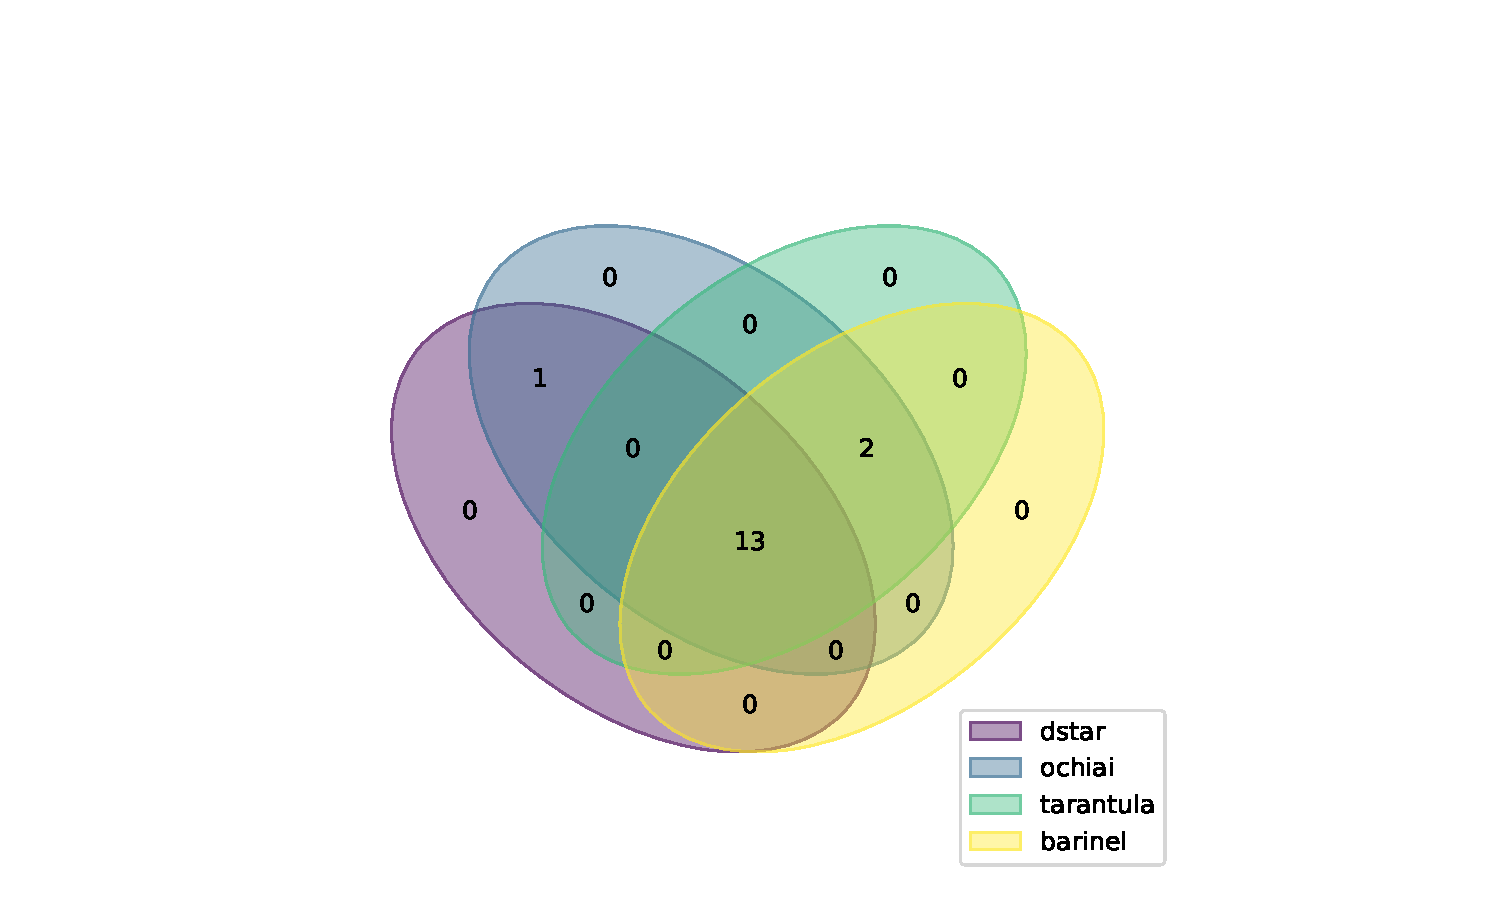
\includegraphics[width=0.5\textwidth, trim=40mm 0mm 40mm 30mm, clip]{figures/sherloc/venn_sbfls.pdf}
\caption{Venn-diagram of flaky classes ranked in the top 5 by the four SBFL \formulas.} 
\label{fig:sbfl_venn}
\end{figure}

\begin{tcolorbox}[
    left=2pt,right=2pt,top=2pt,bottom=2pt,
    arc=0pt,
    boxrule=1.2pt
]
\textbf{RQ1:} 
Using SBFL, we were able to localise flaky classes by inspecting only 21-24\% (6-7\%) of classes covered by flaky tests on average (median). With Ochiai, flaky classes are ranked at the top and in the top 10 for 16\% and 55\% of total flaky commits. 
\end{tcolorbox}

\subsection{RQ2: Code and Change Metrics}

Table~\ref{tab:RQ2} shows the evaluation results for GP-evolved models using SBFL scores with change and code metrics.
The table shows that the addition of signals from change and size metrics leads to an improvement in the identification of flaky classes.
In particular, by adding change metrics, the percentage of classes ranked at the top reaches 24\%. 
This percentage is much higher than the maximum percentage achieved with SBFL alone, which is 16\% with Ochiai.
On the contrary, we do not observe any significant improvements in the number of flaky tests ranked in the top 10 or top 5. 
Combined, these results imply that these change and size metrics can give additional signals that break ties between the classes located near the top, allowing developers to identify the exact cause of flakiness more precisely.
The comparison with the results of GP with only SBFL \formulas in Table~\ref{tab:RQ1-GP} further supports the usefulness of change and size metrics.
Specifically, by adding change and size metrics, the percentage of flaky classes ranked at the top ($acc@1$) goes from 13\% to 24\% and 18\%, respectively. In addition, average $R_{wef}$ improves 5\% with change metrics and 4\% with size metrics. 

With regard to flakiness metrics, their combination with SBFL scores does not lead to any notable improvements in the ranking of classes at the top. 
The percentage of classes at the top is 11\% and the percentage of classes in the top 10 is 53\%.
One possible explanation for this is that our flakiness metrics are derived from a flakiness taxonomy that focuses on the test instead of the CUT.
Hence, using metrics derived from such categories may not be helpful in the identification of CUT components that are responsible for flakiness.
To alleviate this, future studies should consider categories and metrics that are derived from the CUT, and existing flakiness taxonomies should be updated accordingly.

\begin{table*}[ht]
\caption{RQ2: The contribution of flakiness, change, and size metrics to the identification of flaky classes. 
\label{tab:RQ2}\centering}
\centering
\resizebox{\textwidth}{!}{\begin{tabular}{c|rrrr|rr|rrrr|rr|rrrr|rr}
\toprule
& \multicolumn{6}{c|}{\textbf{SBFL \& flakiness}} & \multicolumn{6}{c|}{\textbf{SBFL \& change}} & \multicolumn{6}{c}{\textbf{SBFL \& size}}  \\
\textbf{Proj. (\#)} & \multicolumn{4}{c}{acc} & \multicolumn{2}{c|}{wef (R$_{wef}$)} & \multicolumn{4}{c}{acc} & \multicolumn{2}{c|}{wef (R$_{wef}$)} & \multicolumn{4}{c}{acc} & \multicolumn{2}{c}{wef (R$_{wef}$)}  \\
& @1 & @3 & @5 & @10 & mean & med & @1 & @3 & @5 & @10 & mean & med & @1 & @3 & @5 & @10 & mean & med \\
\midrule
%

Hbase (8) & 1 & 4 & 5 & 5 & 11.9 (12) & 3 (4) & 2 & 4 & 4 & 5 & 16.9 (13) & 4 (4) & 2 & 4 & 5 & 5 & 11.4 (12) & 3 (3) \\
Ignite (14) & 0 & 2 & 2 & 4 & 230.9 (26) & 63 (4) & 2 & 4 & 4 & 4 & 222.3 (24) & 18 (4) & 1 & 3 & 3 & 5 & 220.1 (24) & 43 (4) \\
Pulsar (10) & 2 & 5 & 6 & 8 & 10.2 (15) & 3 (8) & 3 & 5 & 7 & 9 & 8.0 (12) & 2 (5) & 2 & 5 & 7 & 9 & 6.9 (13) & 2 (6)  \\
Alluxio (3) & 0 & 0 & 1 & 1 & 97.7 (51) & 73 (65) & 0 & 0 & 1 & 1 & 75.7 (49) & 94 (39) & 0 & 0 & 1 & 1 & 90.7 (49) & 77 (58) \\
Neo4j (3) & 1 & 2 & 2 & 2 & 19.3 (42) & 1 (18) & 2 & 2 & 2 & 2 & 6.7 (37) & 0 (9) & 2 & 2 & 2 & 2 & 23.0 (40) & 0 (10) \\

\midrule
Total  (38) & 4 & 13 & 16 & 20 & 99.5 (24) & 8 (8) & 9 & 15 & 18 & 21 & 94.1 (21) & 5 (6) & 7 & 14 & 18 & 22 & 94.3 (22) & 5 (7) \\
Percentage (\%) & \textbf{11} & 34 & 42 & \textbf{53} & - & - & \textbf{24} & 39 & 47 & 55 & - & - & \textbf{18} & 37 & 47 & 58 & - & - \\

\bottomrule
\end{tabular}}
\end{table*}

To further investigate the impact of change and size metrics on the identification performance, we analyse the involvement of each metric in our GP-evolved \formulas. 
Table~\ref{tab:RQ2-distr} shows the frequency of change and size metrics in the GP evolved \formulas generated under the configuration of using SBFL and change metrics (\ie SBFL \& Change) and the configuration of using SBFL and size metrics (\ie SBFL \& Size). 
As shown in this table, both change and size metrics are frequently involved in the final \formulas, confirming that our observed improvement did not come only from using GP.
Based on these results, we posit that change and size metrics can contribute positively to the identification of flaky classes.

\begin{table}[ht]
\caption{Frequency of metrics in GP-evolved \formulas (from 0 to 1). `Changes' and `Dev' denote \textit{`Unique Changes'} and \textit{`Developers'}, respectively. The column `SBFL' contains the average frequency of the four SBFL metrics. 
\label{tab:RQ2-distr}}
\centering
\scalebox{0.85}{
\begin{tabular}{l|c|ccc|ccc}
\toprule
 & \textbf{SBFL} & \textbf{Changes} & \textbf{Dev} & \textbf{Age} & \textbf{LOC} & \textbf{DOI} & \textbf{CC} \\
\midrule
SBFL \& Change & 0.45 & 0.50 & 0.37 & 0.53  & - & - & - \\
SBFL \& Size & 0.50 & - & - & - & 0.71 & 0.37 & 0.73 \\
\bottomrule
\end{tabular}
}
\end{table}


\begin{tcolorbox}[
    left=2pt,right=2pt,top=2pt,bottom=2pt,
    arc=0pt,
    boxrule=1.2pt
]
\textbf{RQ2:} 
The augmentation of Spectrum-Based Fault Localisation with change or size metrics lets more flaky classes be ranked near the top; by adding change metrics, we can rank 24\% flaky classes at the top. In contrast, metrics specific to flakiness categories do not provide any beneficial signals to the identification approach. 
\end{tcolorbox}

\subsection{RQ3: Ensemble Method}

Table~\ref{tab:RQ3-voting} presents the evaluation results for the voting method with 60 GP-evolved models, half from using SBFL and change metrics and the other half from using SBFL and size metrics.
We decided to exclude the models that build on flakiness metrics since their usage did not improve the performance any further.
As explained in Section~\ref{sec:rq3_ensemble_method}, there can be a case where none of the participating models succeeds to vote for the true candidate since individual models vote only for those ranked within the top n. For this case, we report the median of all rankings of the models as an alternative. 

The results show that the voting step further improves the ranking results.
The most notable improvement is the accuracy at the top 3, which reaches 47\%. Although the improvements in the other accuracy metrics are not as noticeable as what we have seen in the accuracy at the top 3, there are constant improvements over the results without voting. 
The average of wasted effort remains almost the same while the median improves from the voting, dropping to 3.5. These results imply that the voting allows those near the top to shift further to higher ranks based on the agreement among the models that exploit and capture different features of flaky classes.
Nonetheless, the constant improvements in $R_{we}$, both per project and in total, suggest that through the voting, we can rank flaky classes further near to the top; for example, in Alluxio, where $R_{wef}$ is always near 50, average $R_{wef}$ reduces to 22 and its median to 10. 
These results imply that voting can leverage the complementarity between different models, further improving the localisation of flakiness.

\begin{table}[ht]
\caption{RQ3: The effectiveness of the voting between 60 different GP-evolved models, 30 from SBFL with change metrics, and 30 from using SBFL with size metrics. `Perc' denotes Percentage \label{tab:RQ3-voting}\centering}
\centering
\scalebox{0.9}{
\begin{tabular}{l|r|rrrr|rr}
\toprule
\textbf{Project} & \textbf{Total} & \multicolumn{4}{c|}{\textbf{acc}} & \multicolumn{2}{c}{\textbf{wef (R$_{wef}$)}} \\
& & @1 & @3 & @5 & @10 & mean & med \\
\midrule

Hbase & 8 & 3 & 5 & 6 & 6 & 9.62 (12) & 1.5 (2) \\
Ignite & 14 & 2 & 4 & 4 & 4 & 228.61 (24) & 17.5 (4) \\
Pulsar & 10 & 3 & 6 & 7 & 9 & 7.30 (12) & 2.0 (5) \\
Alluxio & 3 & 1 & 1 & 1 & 2 & 61.83 (22) & 9.0 (10) \\
Neo4j & 3 & 1 & 2 & 2 & 2 & 19.67 (42) & 1.0 (18) \\

\midrule
Total & 38 & 10 & 18 & 20 & 23 & 94.61 (19) & 3.5 (5) \\
Perc (\%) & 100 & 26 & \textbf{47} & 53 & 61 & - & - \\

\bottomrule
\end{tabular}
}
\end{table}

\begin{tcolorbox}[
    left=2pt,right=2pt,top=2pt,bottom=2pt,
    arc=0pt,
    boxrule=1.2pt
]
\textbf{RQ3:} 
A voting between models based on SBFL, change, and size metrics, provides the best ranking for flaky classes.
47\% of flaky classes are ranked in the top 3 and 26\% of them are ranked at the top. The average $R_{wef}$ further reduces to 19, highlighting the practical usefulness of our approach.  
\end{tcolorbox}

\subsection{RQ4: Flakiness Categories}
Table~\ref{tab:RQ4} presents the performances of the voting method on the different flakiness categories encountered in our dataset.
The \textit{``Ambiguous"} category represents cases where the flaky tests could not be assigned to any of the known flakiness categories.
First, we observe that the most common categories are Concurrency and Asynchronous Waits.
This aligns with observations from previous studies~\cite{Luo2014,Lam2020a,Eck2019} and confirms that the taxonomy adopted for our metrics is adequate for our distribution.
Furthermore, we observe a discrepancy between the performances in different categories.
Classes responsible for Async Waits are well identified with 80\% of the classes in the top 10, and 30\% of them at the top.
Classes responsible for Concurrency also show good performances with 50\% of them in the top 10, and 38\% of them at the top; the average $R_{wef}$ is below ten, eight precisely, meaning we can locate flaky classes by inspecting less than 10\% of the total number of the classes covered by flaky tests. 

Categories such as Time and I/O show much lower performances, with 33\% and 0\% of flaky classes in the top 10, respectively.
Nevertheless, given the low number of instances for these categories, it is hard to discuss or generalise their results.
With only two instances, the category Unordered Collections shows curious results as one class is ranked second and the other one ranked 663. 
To understand the reasons behind the bad ranking, we manually inspected this case\footnote{\url{https://github.com/apache/ignite/commit/188e4d52c2}}.  
We found that the concerned test, \texttt{testUnstableTopology}, was executed twice due to a retry mechanism. Both executions led to failure, but interestingly, we found that the two failures have different causes. One of them is due to a lack of context initialisation and is likely to be the reason behind flakiness. 
As the two failure causes are different, the coverage is also different in them.
Specifically, one of the failures  did not cover the flaky class, and as the coverage of this failure was leveraged in the SBFL, the flaky class was not considered suspicious.
We discuss other reasons responsible for poor ranking in Section~\ref{sec:sherloc-discussion}.

\begin{table}[ht]
\caption{RQ4: The effectiveness per flakiness category \label{tab:RQ4}\centering}
\centering
\scalebox{0.8}{
\resizebox{\textwidth}{!}{\begin{tabular}{l|rrrr|rr}
\toprule
\textbf{Flakiness} & \multicolumn{4}{c|}{\textbf{acc}} & \multicolumn{2}{c}{\textbf{wef (R$_{wef}$)}} \\
\textbf{Category} & @1 & @3 & @5 & @10 & mean & med \\
\midrule

Concurrency (16) & 6 (\textbf{38}) & 7 (44) & 7(44) & 8 (\textbf{50})& 147.53 (27) & 9.5 (9) \\
Async wait (10) & 3 (\textbf{30}) & 6 (60) & 8 (80) & 8 (\textbf{80})& 21.05 (8) & 1.5 (3) \\ 

Ambiguous (4) & 1 (25) & 2 (50) & 2 (50) & 3 (75)& 18.88 (5) & 3.5 (5) \\
Time (3) & 0 (0) & 0 (0) & 0 (0) & 1 (\textbf{33})& 88.33 (16) & 14.0 (10) \\
Network (2) & 0 (0) & 2 (100) & 2 (100) & 2 (100)& 1.00 (10) & 1.0 (10) \\
Unordered  &  &  &  &  & &  \\
collections (2) & 0 (0) & 1 (50) & 1(50) & 1 (50) & 331.5 (33) & 331.5 (33) \\
I/O (1) & 0 (0) & 0 (0) & 0(0) & 0 (\textbf{0})& 12.50 (3) & 12.5 (3) \\
Random (1) & 0 (0) & 1 (100) & 1 (100) & 1 (100)& 2.00 (75) & 2.0 (75) \\

\midrule
Total (39\tablefootnote{One flaky class belongs to two categories: Network and Unordered Collections.}) & 10 & 18 & 20 & 23 & 94.47 (19) & 3.5 (5) \\
Perc (\%) & 26 & 47 & 53 & 61 & - & - \\

\bottomrule
\end{tabular}}
}
\end{table}

\begin{tcolorbox}[
    left=2pt,right=2pt,top=2pt,bottom=2pt,
    arc=0pt,
    boxrule=1.2pt
]
\textbf{RQ4:} 
The most prominent flakiness categories, Concurrency and Asynchronous Waits, are identified effectively, with 38\%
and 30\% of their flaky classes ranked at the top, respectively.
In the Concurrency category, flaky classes are identified by examining 8\% of classes covered by flaky tests on average. 
\end{tcolorbox}
\section{Discussion}
\label{sec:sherloc-discussion}

In this section, we discuss our results in light of the existing literature on test flakiness and fault localisation.
Our approach uses existing fault localisation techniques to identify flaky classes in the CUT.
While we leverage various data sources, the main strength of our approach comes from adopting existing SBFL techniques, as explained in RQ2. The effectiveness of other data, such as change metrics, is limited in providing additional signals that break ties between the classes already ranked near the top. Hence, the performance of our approach largely depends on the applicability of SBFL to our flaky class identification problem.  


The flaky class identification problem and traditional fault localisation problems are similar in the way they are debugged (\ie from the reproduction and cause identification to the fix). As described in~\ref{sub:rq1_effectiveness}, this resemblance allows us to redefine SBFL techniques to identify flaky classes instead of faulty ones. Nevertheless, there is one significant difference between them: the characteristics of a test suite. 

Many fault localisation studies assume a test to cover a single functionality, and the subjects they studied often follow this assumption~\cite{Lou:2021:fse,DeepFL,Wen:2019:tse}.
In contrast, we did not consider such an assumption for test subject selection to reflect a realistic scenario of flaky test failure. 
This difference may restrict the applicability of existing fault localisation techniques to the flaky class identification problem, especially test coverage-based techniques, such as SBFL.
Indeed, although we identified 26\% and 61\% of flaky classes at the top and within the top 10, we failed to reach the performance reported in prior work on fault localisation~\cite{wong2016survey}. Hence, we investigate
the diagnosability of the test suite of our subjects using the Density, Diversity, and Uniqueness (DDU) metric~\cite{perez:2017:icse}. 

DDU diagnoses the adequacy of SBFL for a software system by considering three properties of its test suite: Density, Diversity, and Uniqueness. Each property covers a distinct feature of a test suite, and DDU is computed as the multiplication of these three properties. 
Density evaluates how frequently a code entity, in our case a class, is covered by tests. Diversity is about whether tests cover code entities in a diverse fashion. Lastly, uniqueness guarantees that different code entities are covered by different sets of tests. 
All these three components of DDU have values between 0 and 1. The higher the DDU is, the more adequate the test suite is for SBFL. 

Table~\ref{tab:DDU} presents DDU values for the five projects analysed in this study. While all five projects generally have high diversity values (\ie all above 0.9), they have relatively low uniqueness and density values, which results in low DDU scores. Among the five projects, Pulsar has the highest DDU score of 0.289, followed by Neo4j, Alluxio, Ignite, and Hbase. Since both Neo4j and Alluxio have only three flaky classes, which might be too small to discuss the identification results, we will skip these two for the following discussion.
Among the remaining three projects, all our flaky class identification methods, ranging from pure SBFL to voting, perform the best on Pulsar, the one with the highest DDU score, in \textit{acc@n} and \textit{wef}. For instance, even the pure SBFL approach that often performs the worst successfully localised nine out of ten flaky classes of Pulsar within the top 10 and more than half within the top five. The same trend was observed in both GP and voting-based methods.
Compared to HBase, while Ignite has a slightly higher average for the DDU score, it has a far lower Uniqueness score (\ie 0.188 for Ignite and 0.413 for HBase). Uniqueness evaluates whether a code entity is distinguishable; we assume that the flaky classes have different coverage than non-flaky classes. Thus, we suspect that Ignite having a lower Uniqueness is why our methods were not as effective on Ignite as on HBase: we have the worst results on Ignite in both absolute (\ie \textit{acc@n} and \textit{wef}) and relative effort (\ie $R_{wef}$). 

Based on these results, we argue that while our outcome may not be as good as those reported by prior fault localisation studies\cite{Yoo:2017ss,sohn-TSE}, that is mainly due to the inherently low diagnosability of a test suite (\eg covering too many classes in the same fashion). This test-suite adequacy issue commonly exists in the fault localisation field\cite{sohn2021assisting} and is not limited to flaky class identification. Hence, we posit that the performance of our approach can improve along with the advances in fault localisation techniques. 

\begin{table*}[ht]
\caption{DDU metrics for the analysed test suites. \label{tab:DDU}}
\centering
\resizebox{\textwidth}{!}{
\begin{tabular}{l|ccc|ccc|ccc|ccc}
\toprule
\textbf{Project} & \multicolumn{3}{c|}{\textbf{Density}} & \multicolumn{3}{c|}{\textbf{Diversity}} & \multicolumn{3}{c|}{\textbf{Uniqueness}} & \multicolumn{3}{c}{\textbf{DDU}}\\
& min & max & mean & min & max & mean & min & max & mean & min & max & mean \\
\midrule

Hbase & 0.049 & 0.477 &  0.248 & 0.995 & 0.999 & 0.997 & 0.188 & 0.553 & 0.413 & 0.021 & 0.116 & 0.091 \\
Ignite & 0.368 & 0.993 & 0.736 & 0.918 & 1.000 & 0.979 & 0.045 & 0.486 & 0.188 & 0.034 & 0.466 & 0.132 \\
Pulsar & 0.029 & 0.998 & 0.491 & 0.984 & 0.998 & 0.994 & 0.520 & 0.786 & 0.609  & 0.019 & 0.518 & 0.289\\
Alluxio & 0.414 & 0.833 & 0.591 & 0.958 & 0.996 & 0.982 & 0.226 & 0.615 & 0.362 & 0.101 & 0.322 & 0.201  \\
Neo4j & 0.127 & 0.739 & 0.515 & 0.894 & 0.993 & 0.931 & 0.268 & 0.791 & 0.585 & 0.088 & 0.522 & 0.258 \\
\bottomrule
\end{tabular}
}
\end{table*}


In an attempt to shed light on the 15 cases where the class was ranked outside the top 10 by our voting approach, we extended our inspection to reason about such performances. We observed that flaky tests covering a high number of classes are more likely to result in low performances. 
For example, the flaky test \texttt{shutdownDatabaseDuringIndexPopulations} in Neo4j covers 480 classes and its flaky class was ranked 59 by our voting approach whereas the other flaky tests in Neo4j (having their corresponding flaky classes ranked 1 and 2) cover fewer than 10 classes. When we inspect the DDU score of the specific commit that contains this test, it has a relatively low DDU score compared to the other two commits. 
Additionally, most of the mis-ranked classes are found in the Ignite project (10/15), whose DDU score is the second-lowest, and its tests cover on average 492 classes. Due to this consequent number of covered classes, we suspect these tests to be of a higher level, \ie integration or end-to-end tests. 
This aligns with studies highlighting the prevalence of flakiness in integration and system tests~\cite{Kowalczyk2020,Herzig2015}.
Still, our approach does not systematically fail to identify flaky classes covered by higher-level tests as nine of them (flaky test covering more than 100 classes) are listed in the top 10.
\section{Threats to validity}
\label{sec:sherloc-threats}


\paragraph{External validity}
The main threat to the external validity of this study is the dataset size.
To ensure the generalisability of our results, it would have been preferable to include more flaky tests in our experiments. 
Nonetheless, the datasets of flaky tests are generally limited in size due to the elusiveness of flakiness~\cite{habchi2021mutinject,Haben2021,alshammari2021flakeflagger}.
Moreover, as explained in Section~\ref{sec:data_collection}, the requirements of this study limited the set of candidates considerably.
For a commit to be eligible in our study, it needs to have atomic changes fixing flakiness in the CUT.
However, only 24\% of flaky tests actually stem from the CUT, which limits the size of potential subjects~\cite{Luo2014}.
Besides, the creation of our dataset required a substantial amount of manual work to identify suitable commits and perform necessary changes to retrieve coverage matrices.
For instance, for each commit, we had to modify the build script to match \textsc{Gzoltar} requirements, \ie find the test executor version that matches both the program under test and the plugin.
We iteratively removed non-essential listeners and other plugins that could interfere with the instrumentation.
Moreover, we had to find and adapt the execution environment to match the program under test and the testing environment.
%Thus, collecting our dataset, manually analysing the commits, and retrieving the coverage matrices consumed over three person months. 
Finally, compared to the works of Lam~\etal~\cite{Lam2019RootCausing} and Zitfci and Cavalcanti~\cite{De-Flake}, which were conducted on proprietary software, this study is the first to leverage open-source software to localise flakiness root causes.
Thus, our dataset and ground truth can be valuable for future studies on flakiness debugging.


%Other categories

\paragraph{Internal validity}
One potential threat to our internal validity is our definition of flakiness root causes within the CUT, \ie flaky classes.
We rely on flakiness-fixing commits to identify classes that are responsible for flakiness.
%We consider this choice to be the most reasonable provided that no other ground truths exist in the literature.
However, we cannot be certain that (i) the flakiness fix is effective, and (ii) the modified class is the one responsible for flakiness.
Indeed, a study by Lam~\etal~\cite{Lam2020a} showed that developers may wrongly claim that their commits fix flaky tests before realising that the fix is ineffective.
Additionally, there are no guarantees that the classes included in the fix are the ones responsible for flakiness.
Nonetheless, if the class was part of the proclaimed fix, this means that the developers found it, at least, relevant. Hence, its identification by our approach is still helpful for developers willing to understand, debug, and fix flaky tests.

\paragraph{Construct validity} 
%Ground truth: Culprit classes are not accurate
One potential threat to our construct validity is our measurement of the coverage for flaky tests.
A flaky test can pass and fail for the same version of the program, but in practice, it may be extremely difficult to reproduce both the pass and failure~\cite{alshammari2021flakeflagger,Lam2020}.
Hence, a test can be observed as flaky by the project developers and therefore fixed, yet we are unable to reproduce the pass and failure in our experiments even with a large number of reruns~\cite{alshammari2021flakeflagger}.
For this reason, we focused on the available status, \ie pass or failure, and retrieve its coverage.
It is possible that including the coverage of both the pass and failure from the flaky tests might lead to different results with spectrum-based fault localisation.
Thus, we encourage future studies to investigate this direction.
Another possible threat is whether the evaluation results of our approach truly support what we claim. %We use two evaluation metrics, $acc@n$ and $wef$, that can reflect the realistic debugging effort of developers, following the suggestion from Parnin and Orso~\cite{parnin}.
We use two absolute metrics, $acc@n$ and $wef$, that can reflect the realistic debugging effort of developers, following the suggestion from Parnin and Orso~\cite{parnin}, and one relative metric, $R_{wef}$, to compare with the baseline of inspecting classes covered by flaky tests. 
%to show that our approach can give additional guidance to currently available information, such as the list of classes covered by flaky tests. 
\section{Conclusion}
\label{sec:sherloc-conclusion}


%Root causing flaky tests is a young nonetheless important research area. Surveys showed how difficult flakiness debugging can be for developers, even when knowing which test is flaky (post-detection)~\cite{Eck2019,habchi2021qualitative}. 
%We leveraged our results to elaborate a few recommendations for future works:
We presented the first empirical evaluation of SBFL as a potential approach for identifying flaky classes. We investigated three approaches: pure SBFL, SBFL augmented with change and code metrics, and an ensemble of them. 
We evaluated these approaches on five open-source Java projects. Our results show that SBFL-based approaches can identify flaky classes relatively well, especially with code and change metrics, suggesting that code components responsible for flakiness exhibit similar properties with faults. This finding highlights the potential of existing fault localisation techniques for flakiness identification. At the same time, the results show that flaky tests can have unique failure causes that may mislead any coverage-based root cause analysis, stressing the need to consider these flakiness-specific causes in future studies.
%In summary our conclusions are:
%\begin{itemize}[wide=0pt,noitemsep,topsep=0pt]
%     \item We showed that flakiness debugging techniques can rely on SBFL and metrics that are commonly adopted in defect prediction, to identify flaky components. This fact suggests that code components responsible for flakiness can be localised effectively as they exhibit similar properties with faults. 
%     
%    \item We found that some flaky tests have different failure causes, which could mislead any coverage-based root cause analysis. Future studies should account for these peculiarities while localising flaky causes. 
%    
%    \item Flaky tests of different categories manifest differently in the CUT and coverage-based approaches may not be adequate for all of them. This implies that researchers should take into account the different flakiness categories when devising mitigation strategies and tools.
%    
%    \item Metrics derived from test flakiness categories did not show an impact on the identification of flaky classes. Future studies should investigate the manifestation of flakiness in the CUT and not solely the test. This would allow the inference of metrics that better reflect flakiness in the CUT.
%\end{itemize}

Our study forms the first step towards flakiness localisation. We believe that there is a lot of room for improvement and encourage future studies to explore additional techniques, fault prediction metrics, and devise techniques that can further improve and support flakiness localisation. 



	\section{Conclusions}

We presented HPath, a novel DOM-based locator strategy to generate location paths more flexible for web testing. We have compared its potential to extract properties from the HTML document and its fragility under SUT evolution against state-of-the-art algorithm Robula+. Our results show that when HTML5 semantics are present, HPath can exploit rendered properties of web elements to generate expressive locators in 73.35\% reducing locator breakages from 64.99\% when relying on attribute properties to 0.49\% with rendered properties. However, in its current form, it is not always able to extract rendered properties to create good location paths and leaks the hierarchical structure of the DOM for 41.48\% of the elements.

While HPath offers clear advantages in its expressiveness (only relying on rendered properties) and flexibility (when compared to Robula+), it suffers from some limitations. Indeed, relying on very specific predicates, the approach is not always able to generate short and expressive location paths, which might expose more of the internal hierarchy of the \gls{html} document. This effect is exacerbated when the targeted page is not relying on the current \gls{html}5 standards. However, despite this limitation, our results show that relying on the structure of the rendered \gls{dom} still remains better than exploiting the internal attributes of the elements from the \gls{html} document.
	
	% \backmatter
\end{document}